\documentclass[letterpaper,12pt]{report}
\usepackage[utf8]{inputenc} \usepackage[top=2.cm, bottom=2cm, left=2cm, right=2cm]{geometry} 
\usepackage{mathrsfs} 
\usepackage{palatino} 
\usepackage[font=it]{caption}
\usepackage{graphicx,amsmath,amssymb,rotating,booktabs,url}	\DeclareUrlCommand\url{\def\UrlLeft{<}\def\UrlRight{>}\urlstyle{tt}}  
\usepackage{upgreek}
\usepackage[style=/home/filip/d/biblatex-phys/phys, articletitle=true, biblabel=enumerate, chaptertitle=true, pageranges=true, 
			sorting=none, isbn=false, url=false, doi=false, eprint=false, hyperref=true, firstinits   = true]{biblatex}
\addbibresource{fdphd.bib}


\newcommand{\E}{\mathbf{E}}
\newcommand{\D}{\mathbf{\tilde{D}}}
\newcommand{\Dsd}{\mathbf{D}}
\newcommand{\B}{\mathbf{B}}
\newcommand{\HH}{\mathbf{\tilde{H}}}
\newcommand{\HHsd}{\mathbf{H}}
\newcommand{\epsrl}{\varepsilon_r}
\newcommand{\murl}{\mu_r}
%\newcommand{\epsrl}{\varepsilon^{\rm(Loc)}_r}
%\newcommand{\murl}{\mu^{\rm(Loc)}_r}
\newcommand{\Neff}{N_{\text{eff} }}
\newcommand{\Zeff}{Z_{\text{eff} }}
\newcommand{\eeff}{\varepsilon_{\text{eff} }}
\newcommand{\meff}{\mu_{\text{eff} }}
\newcommand{\ii}{{\mathrm i}}
\newcommand{\rr}{{\mathbf{r}}}
\newcommand{\brho}{\boldsymbol{\rho}}
\newcommand{\kk}{{\mathbf{k}}}
\newcommand{\KK}{{\mathbf{K}}}
\newcommand{\epsr}{{\varepsilon_r}}

\newcommand{\add}[1]{\color{blue}#1\color{black}{}}
\newcommand{\rmv}[1]{\color{grey}\ensuremath{\vdash}#1\ensuremath{\dashv}\color{black}{}}
\newcommand{\mdf}[1]{{\color{red}#1}}
\newcommand{\coloruse}{\marginpar{\scriptsize
\add%
{added}\\ \mdf%
{modified}\\ \rmv%
{deleted} }}



%\makeatletter
%\newcommand{\bfgreek}[1]{\bm{\@nameuse{up#1}}}
%\makeatother
%\parindent=0pt
%\newcommand{\um}{\mbox{$\bfgreek{mu}$m}}

% TODO we refer to tunability - complete it in the rest of the document!!
%% TODO unify impedance as `Z', not `z'

% TODO check if the wavenumber K~/ (2pi/a) is correct
% unify the terminology "band diagram" - "dispersion curves"
% TODO incorporate the text of our 2014 OpEx paper into the rest
%


%% MŠindler: Contents
%%		Preface
%%		Introduction (general diel properties, props of SCs)
%%		Experimental setup (..
%%		Yeh formalism
%%		Transmission in zero magnetic field
%%		Transmission in non-zero mag f
%%		Conclusions
%%		List of tables, symbols; Bibliography; Selected publications (p. 89)

\newcommand{\um}{\mbox{$\upmu$m}}

\newcommand\WorkTitle{Metamaterials for the terahertz spectral range}
\newcommand\FirstandFamilyName{Filip Dominec}
\usepackage[unicode=true,pdftitle={\WorkTitle}, pdfauthor={\FirstandFamilyName}, bookmarks=true, colorlinks=true, breaklinks=true, urlcolor=black, citecolor=black, linkcolor=black, breaklinks=true, plainpages=false,pdfpagelabels=true] {hyperref}

\begin{document}
\begin{center}
	\Large{\textbf{
Czech Technical University in Prague\\
Faculty of Nuclear Sciences and Physical Engineering\\ 
%Department of Physical Electronics\\
}}
 \vspace{3cm}

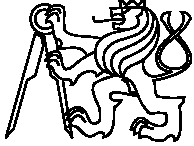
\includegraphics[width=5cm]{img/LogoCVUT}
\vspace{2cm}

\huge{\textbf{\scshape Dissertation thesis}}\\
\vspace{5mm}
{\LARGE\textbf{Metamaterials for the terahertz spectral range\\}}
\end{center}

\date{ } 			


 \vfill
\begin{minipage}{.99\textwidth}
\Large{\textbf{Prague 2016}} \hfill \Large{\textbf{Filip Dominec}}
\end{minipage}


\thispagestyle{empty} \newpage \setcounter{page}{1}

% --------------------------------------------------------------------------------
\chapter*{Bibliografický záznam}
 %\begin{tabular}{rl}
 %Author: 	&\textbf{Filip Dominec}\\
 %Advisor: 	&\textbf{Mgr. Filip Kadlec, Dr.}\\
 %Consultant: 	&\textbf{Doc. Ing. Ivan Richter, Dr.}\\ 
 %Year:		&\textbf{2015}\\
 %\end{tabular}

\bgroup \def\arraystretch{1.5}
\noindent\begin{tabular}{p{.25\linewidth}p{.7\linewidth}}
	Autor:				&\textbf{Ing. Filip Dominec} \\ 
					~	&České vysoké učení technické v Praze\\ 
					~	&Fakulta jaderná a fyzikálně inženýrská\\  
					~	&Katedra fyzikální elektroniky\\
Název práce:			&\textbf{Metamateriály pro terahertzovou spektrální oblast} \\
Studijní program:		&\textbf{Aplikace přírodních věd} \\
Studijní obor:			&\textbf{Fyzikální inženýrství} \\
Školitel:				&\textbf{Mgr. Filip Kadlec, Dr.} \\
					~	&Fyzikální ústav\\ 
					~	&Akademie věd České republiky\\  %Na Slovance 2,  182 21 Praha 8, Czech Republic 
Školitel specialista:	&\textbf{Doc. Ing. Ivan Richter, Dr.} \\
					~	&České vysoké učení technické v Praze\\ 
					~	&Fakulta jaderná a fyzikálně inženýrská\\  
					~	&Katedra fyzikální elektroniky\\
Akademický rok:			&\textbf{2015/16} \\			%% TODO is this the correct format?
Počet stran:			&\textbf{\pageref{enddocument}} \\  %% TODO shall give the overall page number or just that of the authored text?
Klíčová slova			&\textbf{metamateriály, fotonické krystaly, terahertzová technologie, elektrodynamické simulace, homogenizace efektivních prostředí} \\
\end{tabular}
\egroup

\thispagestyle{empty} \newpage

% --------------------------------------------------------------------------------
\chapter*{Bibliographic entry}
\bgroup \def\arraystretch{1.5}
\noindent\begin{tabular}{p{.25\linewidth}p{.7\linewidth}}
Author:					&\textbf{Ing. Filip Dominec} \\
					~	&Czech Technical University in Prague\\
					~	&Faculty of Nuclear Sciences and Physical Engineering\\ 
					~	&Department of Physical Electronics\\
Title of Dissertation:	&\textbf{Metamaterials for the terahertz spectral range} \\
Degree Programme:		&\textbf{Application of natural sciences} \\
Field of Study:			&\textbf{Physical engineering} \\
Supervisor:				&\textbf{Mgr. Filip Kadlec, Dr.} \\
					~	&Institute of Physics\\ 
					~	&Academy of Sciences of the Czech Republic\\  %Na Slovance 2,  182 21 Praha 8, Czech Republic 
Supervisor specialist:	&\textbf{Doc. Ing. Ivan Richter, Dr.} \\
					~	&Czech Technical University in Prague\\ 
					~	&Faculty of Nuclear Sciences and Physical Engineering\\  
					~	&Department of Physical Electronics\\
Academic Year:			&\textbf{2015/16} \\
Number of Pages:		&\textbf{\pageref{enddocument}} \\
Keywords				&\textbf{metamaterials, photonic crystals, terahertz technology, computational electrodynamics, homogenization of effective media} \\
\end{tabular}
\egroup
\thispagestyle{empty} \newpage

% --------------------------------------------------------------------------------
%\vspace{30mm}
%\textbf{\huge{Abstrakt} }
%\vspace{-5mm}

%\begingroup \renewcommand{\newpage}{}
\vspace{-20mm}
\chapter*{Abstrakt}
\noindent ~
% TODO přeložit
Při interakci elektromagnetických vln s periodickými strukturami lze pozorovat neobvyklé jevy, jako je záporný index lomu, fotonický zakázaný pás nebo silná prostorová disperze. Tyto struktury mohou být navrženy tak, aby se chovaly žádoucím způsobem, a označují se buďto jako metamateriály nebo jako fotonické krystaly. Část z jejich navrhovaných využití je v technice terahertzových vln, kde můžou překlenout po\-měr\-ně slabé možnosti klasických součástek.  

Teoretický základ práce vychází z elektrodynamiky prostředí s klasickou frekvenční disperzí, která je dále zobecněna na prostředí s prostorovou disperzí a na Blochovu-Floquetovu teorii vln v periodických strukturách. Závěr teoretické části se pokouší vyjasnit pojmy používané v literatuře a ukázat, že myšlenky metamateriálů i fotonických krystalů jsou ve skutečnosti starší, než se často uvádí.

Obecná teorie je doplněna příklady terahertzového chování různorodých periodických struktur, které bylo vypočteno metodou konečných diferencí v časové doméně (FDTD). V některých případech byly její výsledky podloženy jinými simulačními algoritmy nebo měřeními pomocí terahertzové spektroskopie v časové doméně.

Srovnání  různých struktur si klade za cíl srozumitelnou formou prezentovat a vy\-svět\-lit nej\-pod\-stat\-něj\-ší principy. Podobné srov\-nání zřejmě v dosavadní literatuře chy\-bě\-lo. Klíčové vý\-sledky spočí\-vají v popisu přechodu mezi režimy metamateriálu a fotonického krystalu v periodickém poli dielektrických tyčinek a v důkazech toho, že k popisu chování řady uvedených struktur je zcela nezbytné uvažovat prostorovou dispersi. V neposlední řadě práce dokládá možnosti simulačních skriptů, které autor vyvinul a uveřejnil na internetu s úmyslem podpořit další výzkum v této oblasti. 

\vspace{0mm}
%\chapter*{Abstract} 
{\let\clearpage\relax\chapter*{Abstract}}
\noindent
Unusual phenomena such as negative index of refraction, photonic band gaps, or strong spatial dispersion are observed when electromagnetic waves interact with periodic structures. These can be designed to manipulate the wave in an advantageous way, and are known either as metamaterials or photonic crystals. Part of their proposed applications are for the terahertz technology, where they may address relatively poor performance of classical components.

The theoretical background is derived from the electrodynamics of media with classical dispersion, which is later generalized to spatially dispersive media and to the Bloch-Floquet theory of waves in periodic structures. The end of the theoretical part attempts to clarify the terminology used in the literature, and to show that the concepts of metamaterials and photonic crystals are in fact older than is sometimes assumed.

The general theory is complemented with examples of the behaviour of diverse periodic structures in the terahertz range, which was numerically simulated by the finite-difference time-domain method. In some cases, the results of this simulation method were supported by other simulation algorithms or by the experimental measurement by the terahertz time-domain spectroscopy. 

The comparison of different structures encompassed in this thesis attempts to present and explain most relevant principles in a didactic way. Arguably, such a comparison was missing in the previous literature.
The key results are in the description of the transition between metamaterial and photonic crystal regimes in a periodic array of dielectric rods, and in the demonstration of the fact that considering spatial dispersion is essential for the description of the behaviour of many periodic structures.
Last but not least, the thesis demonstrates the capabilities of the simulation environment which the author developed and completely published online to stimulate further research in this field. 

% TODO Z abstraktu musí být zřejmé, co je cílem předložené práce a jakých vědeckých výsledků doktorand osobně dosáhl.
%% + attention was focused to the parts of different topics, where the author's work could contribute with new knowledge
%\endgroup

\thispagestyle{empty} \newpage
% --------------------------------------------------------------------------------
\chapter*{Acknowledgements}
Preparation of this thesis was not without difficulties. However, it appears that overcoming such difficulties is essential to gain some sort of valuable knowledge that can not be conveyed through textbooks, and of experience that can not be gained through straightforward and focused work only.  At the first place I wish to express thanks to my advisor, Dr. Filip Kadlec, and all other people who helped this project to be finished, namely Dr. Christelle Kadlec and doc. Petr Ku\v{z}el  from the Institute of Physics, and doc. Ivan Richter from the Faculty of Nuclear Engineering and Physical sciences, Czech Technical University. 

Discussions with doc. Lukáš Jelínek and prof. Jan Macháč convinced me about the value in proper handling of the theoretical background, which later proved essential for explaining the results of the thesis. During my stay in France in 2013, the collaboration with Dr. Mathias Vanwolleghem not only greatly contributed to my experience with the numerical simulations, but was also very inspiring. 

Almost surprisingly, all my scientific aspirations found a permanent and selfless support of my wife and all family members, who always had patience with my focusing on abstract problems instead of the more practical aims and with my stubborn attitude towards some of their good advices.

The numerical results presented in the thesis could be hardly obtained without the work of hundreds of volunteers contributing to the open-source scientific software: Most of the plots were made using the Matplotlib library \cite{hunter2007} and computations were based on MEEP \cite{oskooi2010meep} and MPB programs \cite{johnson2001mpb}. 

This work was financially supported by the Czech Science Foundation under Grant No. 14-25639S.

\thispagestyle{empty} \newpage



\chapter{Introduction}
The behaviour of electromagnetic waves in periodic media has attracted the human attention for ages, long before anybody perceived that light is an \textit{electromagnetic wave} or that it is the \textit{periodicity} that is responsible for the brilliant and irreproducible colours of opal gemstones and many living creatures, such as various beetles, butterflies, peacocks etc. %{{{
The scientific community started to study the underlying phenomena in the late 19th century when the X-ray scattering was observed on (periodic) crystal lattices and also when the high optical reflection from periodic layers of entirely transparent materials was predicted. % TODO ref
%The technological and scientific boom of the 20th century contributed with many new theoretical approaches, numerical methods and types of periodic structures to the newly born field of \textit{photonics}. With the advent of the 21th century, great progress was also made in the research of \textit{metamaterials}, a specific subset of periodic structures which will be discussed in greater detail in this work. 
% TODO motivation - finish
The key concept in photonic crystal or metamaterial studies is that the electromagnetic properties are defined predominantly by the shape of the structure, while the actual materials that are used to build it can be relatively freely chosen. % This allows one to take into account the technological and economical aspects. 
While it is unlikely that a radically new material will be invented for construction of optical elements, several new phenomena can be obtained by periodic structuring of ordinary materials. The rapid development of this field was enabled by the modern technology of microfabrication, along with the unprecedented power of computers able to predict the structure behaviour.


% TODO introduction ??
% TODO THz science ??
This work focuses on the terahertz (THz) spectral range, which spans roughly from 100 GHz to 10 THz. While the electrodynamic theory presented in this work is scale-invariant and can be used from microwave to optical frequencies, the selected frequency range defined the properties of materials and technological processes available. Compared to the well established optical technology (400---700 THz), the range of materials suitable for THz frequencies gives additional possibilities, such as the use of superconductors, extremely high permittivity dielectrics and tunable ferroelectrics. Additionally, the much longer wavelength of terahertz waves, e.g. 300 $\upmu$m for 1 THz in free space, also enables much easier fabrication of the structures. On the other hand, some materials commonly found in the microwave or optical applications must be avoided, as they exhibit excessively high losses in the terahertz range (such as glass, water, most plastics etc.)

The THz range is located in the spectrum at the boundary of the regions where people use "electronic" or "optical" approaches. At THz frequencies, devices from both paradigms are often seamlessly used together: waves from waveguides can be collimated by lenses, pulses emitted from lumped antenna emitters are detected by electrooptical crystals etc. Yet none of these approaches is optimal for the THz applications; from the electronic point of view, we are for instance still lacking transistors with fast enough response and the microstrip circuits become too lossy at high frequencies. The optical approach is often complicated by the strong wave-optics phenomena such as diffraction, while some light-matter interactions are weaker, limiting the possibilities for e.g. amplitude modulation by Pockels effect. These deficiencies give additional reasons to search for the new possibilities of the photonic crystals and metamaterials operating in the terahertz range.

% TODO THz MM review 


% TODO -> cíle studie a disertace
Many different designs of metamaterials  % and photonic crystals
were proposed in the last decades, part of them being aimed to the terahertz range. %They have been also summed by several books and reviews % TODO refs x5
% lacks:
%		not covering the area of possible structures
%		too much technology?
%		too specific, no comparison with similar structures, different frequency-spatial scalings of the same
%		often missing  cricital discussion of excessive losses, slow response etc.
%		missing proper electrodynamics
One of the aims of the dissertation are to give a comparison of these structures and to point out the profound similarities in their operation, which may not be obvious.  Some of the structures discussed were also manufactured and experimentally characterized during this PhD project. 
The second aim is to investigate the tunability of their properties depending on external parameters, such as temperature, electric and magnetic fields and illumination. %, i.e. to 
Last but not least, the dissertation project involves the development of a reliable platform for numerical simulations of photonic structures, based on freely available code. Thorough the thesis, the results from these simulations will be verified against experimental data and analytic models.
% Based on a firm theory of electrodynamics of periodic structures

%% TODO update 
%In the following section we present a brief overview of the relevant physical theory. We review the propagation of electromagnetic waves in the free space and in simple periodic structures. We  outline the boundary which usually divides the fields of \textit{photonic crystals} and \textit{metamaterials}, trying to support the hypothesis that the theoretical approaches used for each field can be unified and used for the other field as well.
%The next section focuses on the numerical methods we employed to predict experimental results and, most importantly, to understand the physical nature of the predicted phenomena. We provide a comparison of the finite-difference time-domain simulation (FDTD), the plane-wave expansion (PWE) and the transfer matrix method (TMM). We point out the capabilities of each of them and we also show how the results from these different methods can be processed to give comparable quantities.
%The fourth section gives an overview of the experimental techniques that were used to fabricate the samples and measure their response to a broadband terahertz impulse.
%The longest section follows, in which a systematic list of the most important periodic structures is provided along with their electromagnetic behaviour. Through this work we focused on the terahertz spectral range. 
% TODO Where appropriate, we also investigated how this behaviour depends on some external parameter (such as electric field, temperature or illumination) -- in other words, how the \textit{tunability} of the structure can be achieved.
%In the last section, some general conclusions and prospects are drawn.
%}}}



\chapter{Theory}



\add{The theoretical chapter starts with a brief review of \textit{electrodynamics of continuous media}. In its customary form without account for spatial dispersion, this topic is treated in every related textbook, so classical linear electrodynamics is introduced in a minimalistic manner.
%, avoiding many relevant topics such as  TODO, which are not essential for the description of metamaterials.  
This serves as a basis for transforming into the so-called Landau-Lifshitz formulation of electrodynamics for spatially-dispersive media, which is elaborated more in detail.}

\section{Electrodynamics of continuous media} 
\subsection{Electromagnetic wave in vacuum} % FIXME
\paragraph{Maxwell equations}  %{{{
In the realm of classical physics, the electromagnetic phenomena are governed by the \textit{Maxwell equations} in the following form.
We assume here that no free charges and no sources of currents are present: 
\begin{equation} \nabla \cdot  \D = 0, \label{eq_me1}\end{equation}  
\begin{equation} \nabla \cdot  \B = 0, \label{eq_me2}\end{equation}  
\begin{equation} \nabla \times \E = -\frac{\partial \B} {\partial t}, \label{eq_me3}\end{equation}  
\begin{equation} \nabla \times \HH =  \frac{\partial \D} {\partial t}, \label{eq_me4}\end{equation}  
where the $\E$ and $\HH$ are the electric and magnetic vector fields, and $\D$ and $\B$ are the electric and magnetic displacements,
 respectively. These two pairs of field and displacement are related in a similar way as a force is related to the deformation. %% TODO Simovski2007 regards the current J as force, and E as the deformation!
 The \textit{constitutive relations} depend on the properties of the medium the wave propagates in, and in vacuum they take the simplest possible form:
\begin{equation}		\D = \varepsilon_0	\E, \quad\quad\quad						\B = \mu_0			\HH,				 \label{eq_ce}\end{equation}
the $\varepsilon_0 = 8.85\cdot10^{-12}$ F/m being the \textit{vacuum permittivity} and $\mu_0 = 1.25\cdot10^{-6}$ H/m being the \textit{vacuum permeability}. 
Pages \pageref{starttext}--\pageref{endtext} of this thesis will be concerned with computation, interpretation, and experimental verification of the Eq. (\ref{eq_me1}--\ref{eq_me4}) solutions for specific choices of constitutive equations.
\label{starttext}
%}}}
\paragraph{Wave equation in vacuum} %{{{
The pair of first-order differential equations (\ref{eq_me3}, \ref{eq_me4}) can be converted to a single second-order differential equation. To this end, we apply an extra curl operator $\nabla\times$ from the left, and substituting from one equation into the another, we accumulate two curl operators on the left hand side and two derivatives on the right hand side: 
\begin{equation} \nabla\times (\nabla\times \E) = \nabla\times \left(- \frac{\partial \B} {\partial t}\right) = -\mu_0 \frac{\partial}{\partial t} \left(\nabla\times \HH\right) 
= -\mu_0 \frac{\partial^{2} \D}{\partial t^{2}} = -\mu_0 \varepsilon_0 \frac{\partial^{2} \E}{\partial t^{2}}.  \label{eq_elim}\end{equation}
Using the vector calculus identity
\begin{equation} \nabla\times (\nabla\times \E) \equiv \nabla (\nabla \cdot \E) - \nabla^2 \E, \label{eq_rotrot}\end{equation}
we obtain the \textit{wave equation} for the electric field in vacuum: 
\begin{equation}  \nabla (\nabla \cdot \E) - \nabla^2 \E = -\mu_0 \varepsilon_0 \frac{\partial^{2} \E}{\partial t^{2}}.  \label{eq_wave}\end{equation}
%Note this holds for each component of electric field independently. -- NOT: the divergence is not independent of other components
Starting with Eq. (\ref{eq_me4}) instead of (\ref{eq_me3}), the same result could also be easily obtained for the magnetic field $\HH$.
%}}}
\paragraph{Plane wave and sign convention} %{{{
The solutions of the linear wave equation (\ref{eq_wave}) can be decomposed as a sum of \textit{harmonic plane waves}, where \textit{harmonic} means that the amplitude depends on the time $t$ as a harmonic function (e.g. $\sin(t)$). As a \textit{plane wave} we denote such a spatial shape of the fields, that is a function of a single  scalar parameter $\kk\cdot\rr$. Assuming the wave propagates with nonzero velocity, also the spatial dependence on  $\kk\cdot\rr$ must be harmonic, and therefore 

Any other complicated shape of the fields can be decomposed into a linear superposition of more such waves and treated separately \cite{jackson1962book}. 

%Linear electrodynamics is often treated with the 
The electromagnetic field will described as a complex exponential, i.e. as a superposition of two waves differing by a mere quarter-period phase shift, one defining the real part, one the imaginary part of the field. In comparison with the intuitive description of a plane wave in terms of a cosine (or sine) function, the complex notation formally simplifies some mathematical operations, e.g. it allows to easily identify the \textit{phase of a wave as} the exponent (divided by $1/\ii$). 

%% ---- "ENGINEERING" in favor of +iwt , and then perhaps using eps = (eps' - i eps''), or getting along with all-negative eps''
%% https://www.comsol.com/support/knowledgebase/1009/    
%% http://www.tpdsci.com/tpc/RISignDv.php
%% Panofsky & Phillips 1962, p 200 ??
%% ---- "OPTICS" in favor of -iwt, then using the simpler eps = (eps' + i eps'')
 

%% TODO add figure: plane wave
Without loss of generality, we define the electric field as a function of time $t$ and position in space $\rr$, corresponding to a plane wave in the complex notation:
\begin{equation} \E(t, \rr) := \E_0\, e^{\ii\omega t - \ii\kk\cdot\rr} \label{eq_pw}\end{equation}
The plane wave is fully characterised by its \textit{amplitude vector} $\E_0$, \textit{angular frequency} $\omega$ and \textit{wave vector} $\kk$. Note that no restrictions were put to the amplitude vector $\E_0$ so far, thus Eq. (\ref{eq_pw}) can describe both \textit{transverse} wave of any polarization, with $\E_0 \perp \kk$, and \textit{longitudinal wave} with $\E_0 || \kk$.

An important note shall be made on the sign convention for the complex wave. 
We use the `engineering' convention of time dependence: $e^{+\ii \omega t}$, but this is only due to the author's feeling that it is more natural when the wave phase grows in time. 
It is used in  roughly a half of the literature 
(e.g. \cite[p. 9]{engheta2006book}
\cite[pp. 21, 99]{krowne2007book}
\cite[chap. 1-4, 6, 9, 10]{eleftheriades2005book})
.  In the remaining half,
(e.g. \cite[chap. 5, 7, 8]{eleftheriades2005book}),
\cite{jackson1962book}, 
\cite{veselago1968},
\cite{born1999book}, \cite[p. 5]{noginov2011book}), 
the opposite, `optical', convention is used with time dependence of $e^{-\ii \omega t}$. 
The choice of $e^{+\ii\omega t}$ or $e^{-\ii\omega t}$ determines the sign of imaginary part in virtually all complex quantities discussed in this thesis, but with correct interpretation it makes no difference in the physical conclusions as it is only a formal simplification.
In the real world, observable fields do not have any imaginary component so the real part of the result has to be taken. 

In the $e^{+\ii\omega t}$ convention, many parameters of a passive (lossy) system are restricted to have \textit{negative imaginary part}.  An additional complication arises from that a part of the authors using $e^{+\ii\omega t}$ convention wish to represent the imaginary part as \textit{positive}, and they define complex quantities as, e.g., $\varepsilon = \varepsilon' - \ii \varepsilon''$, % TODO verify if this is e.g. "Wallen2011-Anti-resonant response of ..."
thus in their case $\varepsilon''\equiv -\text{Im}(\varepsilon)$. Thorough the thesis, we however represent the real and imaginary parts naturally as $\varepsilon := \varepsilon' + \ii \varepsilon'' $.
%}}}
\paragraph{Dispersion relations in vacuum} %{{{
Only some combinations of ($\E_0, \omega, \kk$) provide a physical solution of the wave equation (\ref{eq_wave}). In vacuum, the allowed solutions can be obtained by first substituting the differential operators by their equivalents for a particular plane wave: %TODO explain
\begin{equation} \nabla \rightarrow -\ii\kk, \quad\quad\quad 
\frac{\partial} {\partial t} \rightarrow \ii\omega, \label{eq_difftok}\end{equation}
so the wave equation (\ref{eq_wave}) can be modified the following way:
$$					\nabla (\nabla \cdot \E) - \nabla^2 \E				  =	-\mu_0 \varepsilon_0 \frac{\partial^{2} \E}{\partial t^{2}},  $$
$$				 -\ii\kk (-\ii\kk \cdot \E)  - (-\ii\kk \cdot -\ii\kk) \E = -\mu_0 \varepsilon_0 (\ii\omega)^2 \E, $$
\begin{equation}   - \kk (\kk \cdot \E)      +          k^2 \E            = +\mu_0 \varepsilon_0 \omega^{2} \E.  \label{eq_wavek}\end{equation}
The solutions of this wave equation for a harmonic plane wave divide into two groups: % TODO add reference that there is no other oslutino
\begin{enumerate}
 \item{\textit{Transverse electromagnetic waves}, with the electric field and wave vector being perpendicular, i.e. $(\kk \cdot \E) = 0$. Therefore, the \textit{dispersion relation} for a transverse plane wave in vacuum is linear:
\begin{equation} k~= \sqrt{\mu_0 \varepsilon_0}\; \omega = \frac{\omega}{c}, \label{eq_dispeq_vac}\end{equation}
where we defined the \textit{speed of light} $c := \frac{1}{\sqrt{\mu_0 \varepsilon_0}}$.
} 
 \item{\textit{Longitudinal electromagnetic waves}, with $\kk\,|| \pm \E$, require the right side of Eq. \ref{eq_wavek} to be zero. In vacuum, there is no such a solution, except for a homogeneous static electric field ($k = 0, \omega = 0$), but they may exist in a dispersive medium.} 
 \end{enumerate}
\begin{figure} \caption{Dispersion curve of a transverse electromagnetic wave in vacuum} \centering 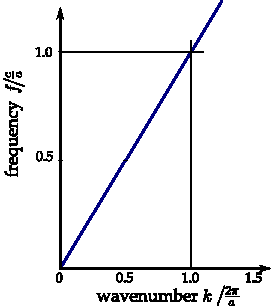
\includegraphics[width=6cm]{img/dispersion_curve_vacuum.pdf} \end{figure}
%}}}

\subsection{Local response of media to the electromagnetic field} \label{loc_response_of_media}
\paragraph{Local response definition} \label{subsection_local_resp} %{{{
In the whole chapter, we expect the medium properties to be time-invariant, linear, and homogeneous (i.e. independent of time, field amplitude and position in space, respectively). 
In this section, we focus on the special case when the medium response in point $\rr$ is not influenced by the electric field in any other point $\brho \neq \rr$. The medium is then said to be \textit{local}. 
For most media found in nature, this approximation is very close to reality and thus numerous electrodynamics textbooks tend to omit the nonlocal effects. 
However using this local theory to a wave propagating through periodic structures has a priori no justification and may lead to completely wrong results. The local theory presented here will serve as a basis for the nonlocal theory developed in following chapters.
% Applying the more familiar local electrodynamics to these structures is a mistake common to many papers. While the local theory is mathematically consistent, it predicts unusual spectral shapes and does not allow their further physical interpretation.

When an electric field $\E$ is applied, the medium responds by a change of the electric displacement $\D$ in a way that is characteristic for it. 
The immediate response of vacuum from the right side of the constitutive equations (\ref{eq_ce}) remains unchanged, but the response of the matter adds a new term called \textit{electric polarisation}. The polarisation is not instantaneous, so it is generally expressed as a convolution of the \textit{electric susceptibility} $\chi_e^{\rm(Loc)}$ with the values of electric field in the previous time $\tau$:
\begin{equation} \D(t,\rr) = \varepsilon_0 \E(t,\rr) + \varepsilon_0 \int_{-\infty}^{t}\chi_e^{\rm(Loc)}(t-\tau)\, \E(\tau,\rr)\,\mbox{d}\tau. \label{eq_loc_chi_convol}\end{equation}
Assume that a harmonic plane wave propagates through the medium, so $\E(t, \rr) := \E_0 \, e^{\ii\omega t - \ii\kk\cdot\rr}$, as given by Eq. (\ref{eq_pw}). This can be inserted in the above equation:
\begin{equation} \D(t,\rr) = \varepsilon_0 \E_0 \, e^{\ii\omega t - \ii\kk\cdot\rr} + \varepsilon_0 \int_{-\infty}^{t} \chi_e^{\rm(Loc)}(t-\tau) \, \E_0 \, e^{\ii\omega \tau - \ii\kk\cdot\rr} \,\mbox{d}\tau. \label{eq_chi_convol_harm}\end{equation}
Substituting $T:=t-\tau$, the exponent can be separated into two parts: one of which factors out of the integral, and the remaining part that turns the convolution into a temporal Fourier transform of the medium response:
$$				 \D(t,\rr) = \varepsilon_0 \E_0 \, e^{\ii\omega t - \ii\kk\cdot\rr} + \varepsilon_0 \int_{-\infty}^{0} \chi_e^{\rm(Loc)}(T) \, \E_0 \, e^{\ii\omega (t - T) - \ii\kk\cdot\rr} \,\mbox{d}T,$$
$$				 \D(t,\rr) = \varepsilon_0 \E_0 \, e^{\ii\omega t - \ii\kk\cdot\rr} + \varepsilon_0 \left( \int_{-\infty}^{0} \chi_e^{\rm(Loc)}(T)  \, e^{-\ii\omega T}\,\mbox{d}T  \right) \E_0 \, e^{\ii\omega t - \ii\kk\cdot\rr}.$$
%% NOTE that the Fourier transform is never subject to the sign change, cf. \ref{eq_kkF}
This is nothing but an application of the convolution theorem: convolution in time domain is equivalent to multiplication the in frequency domain.  %% FIXME normalisation by 2pi?
Consequently we may introduce the local \textit{relative permittivity} $\epsrl(\omega)$ as a function of frequency. It is a property of the medium that determines how strong it develops the electric displacement $\D$ in response to a harmonic wave. From Eq. (\ref{eq_ce}) it is clear that in vacuum,  $\epsrl = 1$.
\begin{equation}  \epsrl(\omega) =   \frac{\D(t,\rr)}{\varepsilon_0 \E(t,\rr)} \biggr|_{\E(t, \rr) := \E_0 \, e^{\ii\omega t - \ii\kk\cdot\rr}} = 1 + \int_{-\infty}^{0} e^{-\ii\omega T} \,\chi_e^{\rm(Loc)}(T) \,\mbox{d}T \label{eq_eps_loc}\end{equation}
%% TODO note that this is a complex-valued function, unlike chi_e(loc); and explain why it is so: that it allows to easily pack in also the information about the phase
%}}}
\paragraph{Response of a harmonic oscillator} \label{chap_lorentzmedia} %{{{
\begin{figure}[t] \caption{\textbf{a)} Illustration of how a simplified medium may respond to an electric field impulse in the shape of Dirac delta function  $E(t) = \delta(t)$. The response is composed from an instantaneous part from vacuum, $\delta(t)$, and from a delayed ringdown of one damped harmonic oscillator, described by $\chi_e^{\rm(Loc)}(t) := 2\pi \sin(2\pi t)\,e^{-x/2}$; \textbf{b)} The corresponding local permittivity $\epsrl(\omega)$, computed by Fourier transform of the response. Note that the imaginary part of permittivity is negative due to that the material is lossy (absorbs energy) and that the $e^{\ii\omega t}$ convention is used.} \label{fg_oscillator_spectrum} \centering 
	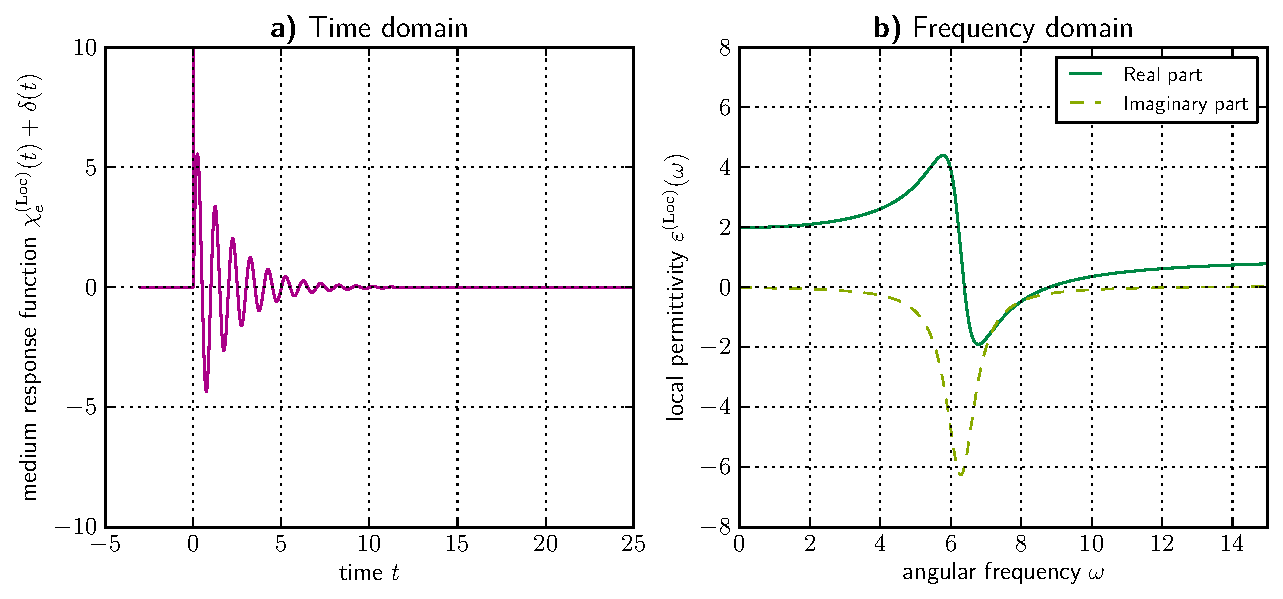
\includegraphics[width=17cm]{img/oscillator_spectrum.pdf}
\end{figure}
The response function $\chi_e(T, \mathbf{R})$ of usual media is composed of different phenomena.  Each of them may react on different time scales, and thus the medium response usually has a relatively complicated shape in the time domain.  However, to a reasonable degree of approximation, each of the contributions can be treated separately, as is demonstrated in the following.

Linear physical systems with an inertial mass, friction force and a restoring force are known as \textit{damped harmonic oscillators}.  This theory applies well to the electrons elastically bound to an atomic nucleus, as well as to the atoms elastically bound to their equilibrium position in the lattice. The molecular rotation can also be modelled as an (possibly overdamped) harmonic oscillator. Even the free electrons in conductive media can fit into the theory of harmonic oscillator provided the restoring force is set to nearly zero. The response of a harmonic oscillator is easy to describe both in time domain and frequency domain, even without the explicit use of the Fourier transform from Eq. (\ref{eq_eps_loc}). The harmonic oscillator model thus becomes a convenient starting point to approximate the response of materials.

A damped harmonic oscillator is described by a second-order differential equation:
\begin{equation} \alpha \frac{\partial^{2} x(t)}{\partial t^{2}} + \beta\frac{\partial x(t)}{\partial t} + \zeta x(t) = f(t). \label{eq_harm_osc}\end{equation}
Provided the driving term on the right hand side  is harmonic $f(t) = e^{+\ii \omega t}$, the system response is also a harmonic function, $x(t) = \chi(\omega) e^{+\ii \omega t}$. The differential equation (\ref{eq_harm_osc}) can be easily solved to show that the complex amplitude of the driven oscillations, $\chi(\omega)$, depends on the angular frequency and on the parameters $\alpha$, $\beta$ and $\zeta$ in the following way:
\begin{equation} \chi(\omega) \equiv \frac{x(t)}{f(t)} = \frac{1}{\zeta-\alpha\omega^{2} + \ii\omega\beta}  = \frac{\alpha^{-1}}{\frac{\zeta}{\alpha}-\omega^{2} + \ii\omega\frac{\beta}{\alpha}}. \label{eq_harm_osc_result}\end{equation}
The physical meaning of $\alpha$, $\beta$ and $\zeta$ is of little importance in this text, but without loss of generality the result of Eq. (\ref{eq_harm_osc_result}) can be rewritten into
\begin{equation} \chi(\omega) = \frac{F}{\omega_0^{2}-\omega^{2} + \ii\omega\gamma}, \label{eq_harm_osc_rewritten}\end{equation}
where the physical interpretation of the three (real and positive) parameters is as follows:
\begin{itemize}
 \item{$\omega_0 = \sqrt{\zeta/\alpha}$ is the angular \textit{frequency of resonance}, at which the response is pure imaginary and usually its modulus $|\chi(\omega=\omega_0)|$ is near its maximum.} 
 \item{$\gamma = \zeta/\alpha$ is the \textit{damping rate}. In time domain, it determines the time constant of exponential amplitude decay. In frequency domain, it is roughly proportional to the resonance width. } 
 \item{$F = \alpha^{-1}$ is the \textit{oscillator strength}, determining the amplitude of the response function.}
 \end{itemize}


\paragraph{Permittivity of Lorentz media} Within the approximation of relatively weak fields, the oscillators act independently of each other.
The response of usual media in frequency domain can thus be decomposed with acceptable precision into a sum of $M$ independent harmonic oscillators, each $m$-th oscillator having the resonance angular frequency $\omega_{0m}$, damping rate $\gamma_m$ and strength $F_m$.
The permittivity function of the material is a solution of the differential equation of a damped harmonic oscillator, driven by a harmonic source:
\begin{equation} \epsrl(\omega) = 1 + \sum_{m=1}^M \frac{F_m}{\omega_{0m}^2 - \omega^2 + \ii\omega\gamma_m} \label{eq_lorentz_eps}\end{equation} %% TODO fix sign; TODO what about eps0 before summation?
Advancing from the general formulation in Eq. (\ref{eq_eps_loc}) to the Lorentz oscillator model in Eq. (\ref{eq_lorentz_eps}) is of great importance for theoretical interpretation of the material response, and it has also become a framework for description of periodic structures even in the presence of spatial dispersion.  %% clumsy - remove this sentence?
An example of the time- and frequency-domain response of a medium with one harmonic oscillator in is Fig. \ref{fg_oscillator_spectrum}.
% It is also the way how one communicates the material definition to the numerical simulation software, as described later (in Chap. \ref{chap_fdtd}). 
% TODO decide whether we use exp(i omega t)     -> leads to negative eps''

One can see that each oscillator increases the real part of permittivity, but in the high frequency limit the contribution of the oscillator vanishes. This can be intuitively understood as that at low frequencies $\omega \ll \omega_0$, the system reacts fast enough to simultaneously follow the driving force, whereas at high frequencies  $\omega \gg \omega_0$, the system does not follow the driving force at all.
The contribution of one oscillator to the low-frequency permittivity $\Delta\varepsilon_r(0)$, is inversely proportional to the oscillator restoring force, which links it to the inverse square of the resonance frequency:
\begin{equation} \Delta \varepsilon_r'(\omega\rightarrow0) = \frac{F}{\omega_0^{2}}.  \label{eq_delta_eps} \end{equation}

A more detailed treatment of the theory of the dielectric function $\epsrl(\omega)$ may be found in many textbooks, e.g. \cite[p. 454]{klingshirn2007semiconductor}, \cite{dresselhaus1966optical}. 

We will return to the Lorentz oscillator model also in the Chapter \ref{def_of_mat}, where the shows to be essential for realistic definition of materials for accurate numerical FDTD simulations. The chapter also describes in more detail how the overdamped molecular rotation and the unbound motion of free charges can be easily represented using correct parameters of an oscillator.
%}}}
\paragraph{Permeability of Lorentz media}  %{{{ 
In a manner very similar to the above derivation of the local permittivity, the \textit{local permeability} can be introduced by means a response of the medium to the magnetic field:
\begin{equation} \murl(\omega) = \frac{\B(t,\rr)}{\mu_0\HH(t,\rr)} \biggr|_{\HH(t, \rr) := \HH_0 \, e^{\ii\omega t - \ii\kk\cdot\rr}} = 1 + \int_{-\infty}^{0} e^{-\ii\omega T} \,\chi_m^{\rm(Loc)}(T) \,\mbox{d}T, \label{eq_mu_loc}\end{equation}
where $\chi_m^{\rm(Loc)}(T)$ is the \textit{magnetic susceptibility of medium} and $\HH_0$ is the amplitude of the magnetic field. This obviously results in an expression for the local permeability in the frequency domain:
\begin{equation} \murl(\omega) = 1 + \sum_{m=1}^M \frac{F_m}{\omega_{0m}^2 - \omega^2 + i\omega\gamma_m}, \label{eq_lorentz_mu}\end{equation} %% TODO fix sign; TODO what about eps0 before summation?
where formally the same notation was used as in  Eq. (\ref{eq_lorentz_eps}): $\omega_{0m}$, $\gamma_m$ and $F_m$ are the magnetic oscillator's angular frequency, damping frequency and strength. Unlike the electric response, most ordinary media have either almost no response to the magnetic field % todo CITE
or their response is limited to low frequencies.

%}}}
\paragraph{Kramers-Kronig relations in local media}%{{{
Causality prevents any medium from reacting to the future electric (or magnetic) field, so the integration in Eq. (\ref{eq_loc_chi_convol}) goes up to the current time only, $\tau \in (-\infty, t)$. The response of the medium to a real-valued field must moreover be also real, no matter that the computations are often done with complex field amplitude [Eq. (\ref{eq_pw})] for the sake of convenience. 

Thus, the basic physical laws impose relatively strict constraints to the time-domain response function $f(t)$, which translate into another constraints for the possible shape of the response in frequency domain $F(\omega)$. The intuitive physical derivation is based on the fact that any time-domain response function can be trivially separated into its odd and even parts as 
, as shown in Fig. \ref{fg_kk}. 
\begin{equation}f(t) = f_{odd}(t) + f_{even}(t) = -f_{odd}(-t) + f_{even}(-t) \label{eq_odd_even_decomp}\end{equation}
\begin{figure}[t] \caption{Illustration of how a real causal function $f(t)$ can be decomposed into the odd and even parts, which then yield a pure imaginary and pure real functions in the spectrum, respectively. Mathematically this is expressed in Eqs. (\ref{eq_odd_even_decomp}--\ref{eq_kkresult}).} \label{fg_kk} \centering 
	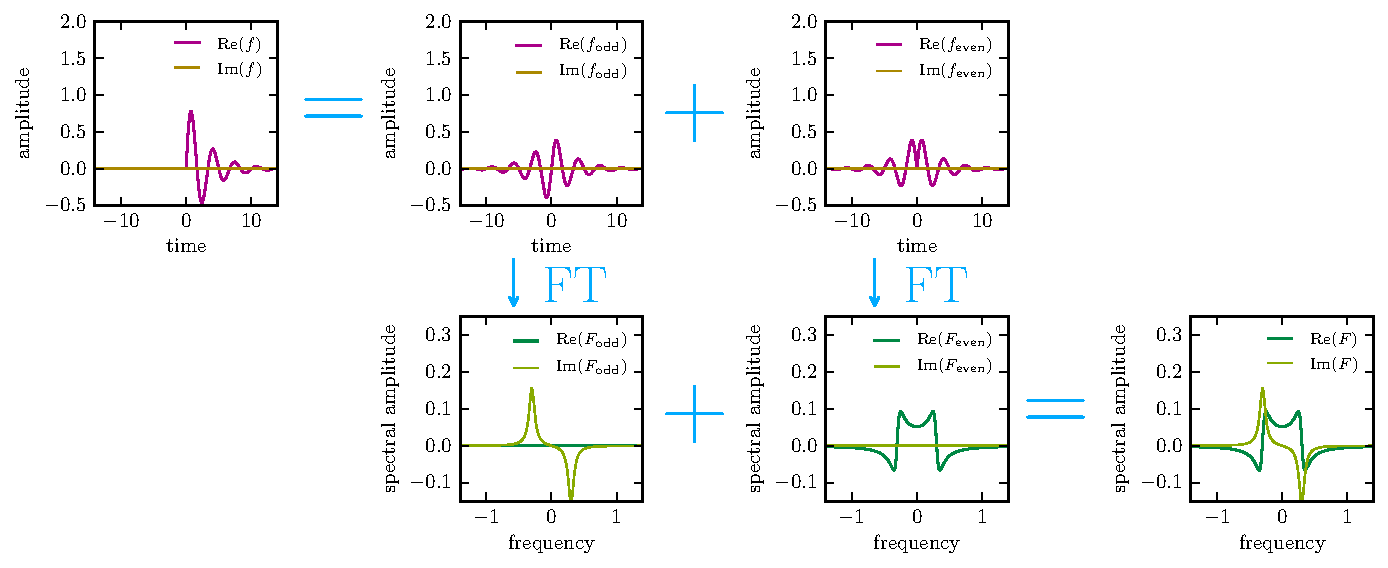
\includegraphics[width=17.5cm]{img/Kramers_Kronig_plot/kk.pdf}
\end{figure}
The Fourier transform of a real odd function is an imaginary function:
%F_{odd}(\omega)=& \int_{-\infty}^{\infty} e^{-\ii \omega t} f(t) \mbox{d}t = \\
		 %=&  \frac{1}{2} \int_{0}^{\infty} e^{-\ii \omega   t } [ f_{odd}(t) + f_{even}(t)] \mbox{d}t 
		   %+ \frac{1}{2} \int_{0}^{\infty} e^{-\ii \omega (-t)} [-f_{odd}(t) + f_{even}(t)] \mbox{d}t  \\
		 %=&  \int_{0}^{\infty} \frac{e^{-\ii \omega t}-e^{+\ii \omega t}}{2} f_{odd}(t) \mbox{d}t 
		   %+ \int_{0}^{\infty} \frac{e^{-\ii \omega t}-e^{+\ii \omega t}}{2} f_{odd}(t) \mbox{d}t  = \\
		 %=&\int_{-\infty}^{\infty} e^{-\ii \omega t} f(t) \mbox{d}t  = \\
		 %=&\int_{-\infty}^{\infty} e^{-\ii \omega t} f(t) \mbox{d}t  = \\
\begin{equation} 
\begin{split} 
F_{odd}(\omega)=& \int_{-\infty}^{+\infty} e^{-\ii \omega t} f_{odd}(t) \,\mbox{d}t = 
		 \int_{-\infty}^{+\infty} \frac{e^{-\ii \omega   t }}{2} f_{odd}(t) \,\mbox{d}t 
		   +  \int_{-\infty}^{+\infty} \frac{e^{-\ii \omega (-t)}}{2} [-f_{odd}(-t)] \,\mbox{d}t  \\
		 =&   \int_{-\infty}^{+\infty} \frac{e^{-\ii \omega t}-e^{+\ii \omega t}}{2} f_{odd}(t) \,\mbox{d}t 
		 = -\ii \underbrace{\int_{-\infty}^{+\infty} \sin(\omega t) \, f_{odd}(t) \,\mbox{d}t}_{\mbox{$\in \mathbb{R}$}},
\end{split} 
\label{eq_kkF}\end{equation}
whereas the Fourier transform of a real even function yields a real function:
\begin{equation} 
\begin{split} 
F_{even}(\omega)= \ldots =   \int_{-\infty}^{+\infty} \frac{e^{-\ii \omega t}+e^{+\ii \omega t}}{2} f_{even}(t) \,\mbox{d}t 
		 = \underbrace{\int_{-\infty}^{+\infty} \cos(\omega t) \, f_{even}(t) \,\mbox{d}t}_{\mbox{$\in \mathbb{R}$}}.
\end{split} 
%% TODO the following is WRONG! see ---->  http://www.thefouriertransform.com/pairs/step.php#signum,  ho3.pdf
\label{eq_kkFeven}\end{equation}
The odd and even components of the time-domain response function correspond to the imaginary and real part of the response spectrum, respectively:
\begin{equation} F_{odd}(\omega) + F_{even}(\omega) = F(\omega), \text{ where } F_{odd}(\omega) = F''(\omega) \text{ and } F_{even}(\omega) = F'(\omega).  \label{eq_kkFodd}\end{equation}
At the same time, $f_{even}(t)$ and $f_{odd}(t)$ are related by having the opposite sign for $t<0$ and the same sign for $t>0$, that is 
\begin{equation} f_{even}(t) = \mbox{sign}(t)\,f_{odd}(t). \label{eq_kkfeven}\end{equation}
Multiplication in the time domain manifests as a convolution in frequency domain
\begin{equation} 
F_{even}(\omega) = \int_{-\infty}^{+\infty}  \frac{-2\ii}{\omega - \Omega} F_{odd}(\omega) \,\mbox{d}\Omega  \equiv  \left[\frac{-2\ii}{\omega}\right]\,\ast\,F_{odd}(\omega),
\label{eq_kkresult}\end{equation} 
where we used the knowledge that the $-2\ii/\omega$ function is the Fourier transform of $\mbox{sign}(t)$. Convolution with this function is also known as the Hilbert transform.% tODO cite

Obviously, Eq. (\ref{eq_kkfeven}) can also be converted to $f_{odd}(t) = \mbox{sign}(t)\,f_{even}(t)$, thus the relation between the real and imaginary part of the response spectrum also holds when $F_{odd}(\omega)$ and $F_{odd}(\omega)$ are exchanged in Eq. (\ref{eq_kkresult}). 

A related mathematical proof of Kramers-Kronig relations can be derived from the analyticity of the response function in the complex plane of frequency. %% TODO cite

%% TODO: why do K-K relations forbid to choose arbitrary phase difference over an unit cell? 
%% ie. Why the Neff can be unambiguously extracted from spectra?
% TODO show how it dictates the "constant area of imaginary part " when resonance Q is changed
%}}}

\subsection{Dispersion relations in local Drude-Lorentz media} \label{disp_rel_local_media}
\paragraph{Lower and upper polariton branches of transverse waves}  % TODO%{{{
Returning to the derivation of dispersion relations, we start with modifying the constitutive relation (\ref{eq_ce}) to a plane wave propagating in a medium:
\begin{equation}		\D := \varepsilon_0\varepsilon_r(\omega)	\E, \quad\quad\quad						\B := \mu_0\mu_r(\omega)		\HH,				 \label{eq_ce2}\end{equation}
with the relative permittivity $\varepsilon_r(\omega)$ and permeability $\mu_r(\omega)$ being two dimensionless functions of frequency, defined in Eq. (\ref{eq_lorentz_eps}, \ref{eq_lorentz_mu}). 
The wave equation (\ref{eq_wavek}) then changes to
\begin{equation} - \kk (\kk \cdot \E) + k^2 \E = \varepsilon_0 \epsrl(\omega) \mu_0 \murl(\omega) \omega^{2} \E, \label{eq_wavek_disp} \end{equation}
which, in the isotropic case, results in the dispersion curve for the transverse electromagnetic wave 
\begin{equation} k~= \sqrt{\varepsilon_0 \mu_0} \sqrt{\varepsilon_{r}(\omega) \mu_{r}(\omega)}\;\omega = \sqrt{\varepsilon_{r}(\omega) \mu_{r}(\omega)}\; \frac{\omega}{c}, \label{eq_dispeq_vac}\end{equation}
with the added frequency-dispersive term responsible for the deviation from the original light line in Fig. \ref{fg_dispersion_vacuum}. 

%TODO FIGURE dispersion curve - scan over resonator strength\\
In the simplest example of a single electric resonance with negligible losses, as in Fig. \ref{fg_dispersion_polariton} % TODO red? line
, the curve is divided into two separate branches. The \textit{lower polariton branch} is below the resonance frequency $\omega_0$ and is characterized by the Lorentz oscillator being in phase with the electric field.
Above $\omega_0$, the dipoles of the Lorentz oscillator can no more follow the electric field and are opposite to it, thus the response of the medium is negative. With further increase of the frequency, the permittivity crosses zero at the frequency $\omega_{\text{L}}$. %, > \omega_0 which allows the transverse wave to propagate. 
where the \textit{upper polariton branch} starts. In case of a Lorentz oscillator unaffected by the presence of others, the difference $\omega_{\text{L}} - \omega_0$ can be computed from the magnitude of the oscillator (using the Lydanne-Sachs-Teller relation).\cite{klingshirn2007semiconductor}

The same behaviour is observed for a single resonance in the permeability $\mu_r(\omega)$, and will be typical also for the spectra of resonances of macroscopic structures described later.

Note that the formation of upper and lower polariton branches can be reinterpreted\cite{landau1984electrodynamics} using the theory of coupled oscillators as the result of \textit{anticrossing} between the oscillator at the frequency $\omega_0$ (forming a horizontal line) and the photon branch (forming a straight growing light-line).

When losses are present, the lower and upper polariton branches are connected by a smooth line of \textit{anomalous} dispersion and very high losses.  % TODO \ref{fg_dispersion_polariton}
%}}}
\paragraph{Longitudinal waves in dispersive media} %{{{
The wave equation in dispersive media, 
\begin{equation} - \kk (\kk \cdot \E) + k^2 \E = \varepsilon_0 \epsrl(\omega) \mu_0 \murl(\omega) \omega^{2} \E, \tag{\ref{eq_wavek_disp} \again} \end{equation}
also allows the existence of longitudinal waves with electric field parallel to the wave vector $\E || \kk$. It was shown earlier that there is no solution for longitudinal waves in vacuum except for static homogeneous field.

If a local medium is assumed, and the wavenumber $k$ is nonzero, such waves can have a solution with nonzero $\E$ when either $\varepsilon_r(\omega)' = 0$, or $\mu_r(\omega)' = 0$. Therefore, the corresponding dispersion curve for a longitudinal wave is a horizontal line at $\omega = \omega_{\text{L}}$, independent of $k$. This would be equivalent to a standing oscillation that maintains the spatial amplitude envelope that was originally excited. 

Different physical phenomena can lead to $\varepsilon_r(\omega)' = 0$, some of which introduce relatively low losses at the corresponding $\omega_{\text{L}}$; namely lattice vibrations in nonconductive crystals or electrons in inductive media (like metals and dilute plasma). At the interface of such media with vacuum or air, another type of waves can be excited with an intermediate frequency $\omega < \omega_{\text{L}}$ that can not propagate in either of the bulk medium. The dispersion curve of such waves is not flat, allowing them to propagate along the interface.
Depending on the mechanism, they are known as \textit{surface phonon-polaritons} or \textit{surface plasmons}, respectively. 
% Are there surface magnons?
% Are there any metamaterials designed for longitudinal waves?
%}}}
\paragraph{Anisotropy of permittivity} \label{par_anisotropy} %{{{
It shall be noted here that permittivity $\epsrl$ was introduced as a scalar, assuming that the vector of electric field $\E$ and electric induction $\D$ are always of the same orientation:
\begin{equation} \D = \varepsilon_0 \epsrl(\omega) \E \equiv \varepsilon_0  
	\left(\begin{array}{ccc} 
			\epsrl(\omega) & 0 & 0  \\
			0 & \epsrl(\omega) & 0  \\
			0 & 0 &\epsrl(\omega)  
	\end{array} \right) \cdot \E
	\label{eq_}
\end{equation}
In some media of lower rotational symmetry (such as many crystals, or liquids under static electric field), the medium response depends on the electric field direction. At the beginning of the chapter, however, we imposed the requirement of \textit{linearity} of the medium. Whatever the linear relation of 
$$\D := \mathcal{L}(\E)$$
is, it must obey the rule
$$\D_1 + \D_2 = \mathcal{L}(\E_1) + \mathcal{L}(\E_2) = \mathcal{L}(\E_1 + \E_2)$$
for any vectors $\E_1, \E_2$. Such a relation can be fully described by a \textit{tensor of permittivity} % TODO cite 
\begin{equation} \D = \varepsilon_0 \epsrl(\omega) \E \equiv \varepsilon_0  
	\left(\begin{array}{ccc} 
	{\epsrl}_{11}(\omega) & {\epsrl}_{21}(\omega) & {\epsrl}_{31}(\omega)  \\
	{\epsrl}_{12}(\omega) & {\epsrl}_{22}(\omega) & {\epsrl}_{32}(\omega)  \\
	{\epsrl}_{13}(\omega) & {\epsrl}_{23}(\omega) & {\epsrl}_{33}(\omega)  
	\end{array} \right) \cdot \E.
	\label{eq_epstensor}
\end{equation}
Elaborate discussion on the restrictions on this tensor and its physical interpretation can be found e.g. in \cite[pp. 678--686]{born1999book}. An analogous treatment can be applied to the magnetic permeability, though it is much less commonly needed.
%}}}
\paragraph{Anisotropic local media}  % TODO%{{{
If the medium response depends on the direction of the field, the dispersion relations can not be directly obtained by substitution into the wave equation. 
It is important to notice that also the leftmost term in 
\begin{equation} - \kk (\kk \cdot \E) + k^2 \E = \varepsilon_0 \epsrl(\omega) \mu_0 \murl(\omega) \omega^{2} \E, \tag{\ref{eq_wavek_disp} \again} \end{equation}
is a linear transformation of the vector $\E$, expressed by the tensor
$$ - \kk (\kk \cdot \E) \equiv 
	-\left(\begin{array}{c} k_x \\ k_y \\ k_z \end{array} \right) \cdot
	\left[\left(\begin{array}{ccc} k_x & k_y & k_z \end{array} \right) \cdot
	\left(\begin{array}{c} E_x \\ E_y \\ E_z \end{array} \right)\right] 
		\equiv
	\left(\begin{array}{ccc} -k_x^2 & -k_x k_y & -k_x k_z \\ -k_y k_x & -k_y^2 & -k_y k_z \\ -k_z k_x & -k_z k_y & -k_z^2 \end{array} \right) \cdot  
	\left(\begin{array}{c} E_x \\ E_y \\ E_z \end{array} \right),
	$$
%$$ k^2 \E \equiv 
%	\left[\left(\begin{array}{ccc} k_x & k_y & k_z \end{array} \right) \cdot 
%	\left(\begin{array}{c} k_x \\ k_y \\ k_z \end{array} \right)\right] \cdot 
%	\left(\begin{array}{c} E_x \\ E_y \\ E_z \end{array} \right),
%	$$
%$$ \mu_0 \varepsilon_0 \omega^{2} \E \equiv 
%	\left(\begin{array}{ccc} k_x^2+k_y^2+k_z^2 & 0 & 0 \\ 0 & k_x^2+k_y^2+k_z^2 & 0 \\ 0 & 0 & k_x^2+k_y^2+k_z^2 \end{array} \right) \cdot  
%	\left(\begin{array}{c} E_x \\ E_y \\ E_z \end{array} \right),
%	$$
The dispersion relation can be reformulated \cite[pp. 667]{born1999book} as a set of linear algebraic equations. 
For simplicity, let us assume the relative permeability $\murl = 1$; then it can be expressed as 
\begin{equation} \det\left[\left(\begin{array}{ccc} 
	k_y^2+k_z^2  	& -k_x k_y 		& -k_x k_z \\ 
	-k_y k_x 		& k_x^2+k_z^2	& -k_y k_z \\ 
	-k_z k_x 		& -k_z k_y		& k_x^2+k_y^2
	\end{array} \right)
-
	\mu_0 \varepsilon_0 \omega^2
	\left(\begin{array}{ccc} 
	{\epsrl}_{11}(\omega) & {\epsrl}_{21}(\omega) & {\epsrl}_{31}(\omega)  \\
	{\epsrl}_{12}(\omega) & {\epsrl}_{22}(\omega) & {\epsrl}_{32}(\omega)  \\
	{\epsrl}_{13}(\omega) & {\epsrl}_{23}(\omega) & {\epsrl}_{33}(\omega)  
	\end{array} \right) \right] = 0, \label{eq_dispdet}\end{equation}
%\begin{equation} \left|\begin{array}{ccc} 
	%k_y^2+k_z^2 - \mu_0 \varepsilon_0 \omega^{2} 		& -k_x k_y 		& -k_x k_z \\ 
	%-k_y k_x 		& k_x^2+k_z^2-\mu_0\varepsilon_0\omega^{2} 		& -k_y k_z \\ 
	%-k_z k_x 		& -k_z k_y		& k_x^2+k_y^2-\mu_0\varepsilon_0\omega^{2}
	%\end{array} \right| = 0, \label{eq_dispdet}\end{equation}
A solution of Eq. \ref{eq_wavek} can exist with nonzero $\E$ if the determinant of the set of three linear equations is zero.
In the most general case, it can be solved by means of numerical algebra software. 
\mdf{
TODO FIGURE: IFC for anisotropic media (are common in nature)\\

TODO FIGURE: IFC for Hyperbolic media (can also be found in nature, in narrow range like near sapphire LO phonno, cite Agranovich)\\
}
%}}}
\paragraph{Isofrequency contours}  % TODO%{{{
%A resonance in local permittivity (or permeability) creates two polariton branches -- thus the dispersion curves can not be expressed as one simple function $\omega(k)$ of the wavevector $k$. It would then appear adequate to treat dispersion curves as a function of frequency, $k(\omega)$, but as is shown below in the presence of nonlocal response, neither $k$ is necessarily a simple function of $\omega$. Also 
It is often important to describe the dispersion curves also for different wave angles, which is the best accomplished by plotting the  %% todo ...real part of ...
frequency $\omega$ as the function of \textit{wave vector} $\kk$. In three dimensions, this would require mapping a function of three independent variables, $\omega(\kk) = \omega(k_x, k_y, k_z)$. However, in most cases the projection of two selected components of $\kk$ is sufficient to understand all relevant phenomena, and naturally it is much easier to visualize.
Such a plot is known as \textit{isofrequency contours} (IFC), or also \textit{equifrequency contours} (EFC). It not only displays rich %?
information about the medium interaction with electromagnetic waves, but also allows for intuitive geometrical analysis of various physical problems. 

The limitation is, however, that IFC plots do not show the imaginary part and thus are applicable to plot dispersion in media with negligible losses only.  % TODO confusing
Each branch also has to be plotted separately, to prevent the contours from overlapping.

\mdf{
TODO FIGURE circular/elliptical/hyperbolic dispersion contours
%% note this is shown in \cite[p. 118]{shalaev2010book}
}
%}}}
\paragraph{Index of refraction, and its applicability}  % TODO%{{{
\mdf{
Noether theorem ->\\
refraction between two isotropic media must keep the phase along boundary   ->  \\
how Snell's arcsin law simply comes out of IFC shape\\

develop the term of index of refraction\\
when does index of refraction make sense? --- strict definition (circular IFC only), weaker definition (tangential and smooth IFC,  works in the limit of small angles, but the beam propagation is not correctly predicted), broadest definition ($k/c\omega$ does not guarrantee prediction of the refraction angle, unusable)

IFCs will be useful also for nonlocal and periodic media later\\


if the surface is smooth, this must hold for any type of media, including anisotropic\\

TODO FIGURE refraction of two media, rgb contours with dispersive angle of refraction
}

%}}}
\paragraph{Phase velocity and group velocity near single resonance}  % TODO%{{{
\mdf{
the discussion regards partial derivative of k-vector by frequency,   d k/d omega ->  \\
derivative of vector function yields another vector function -> \\
show that its magnitude determines the envelope  propagation velocity  \\
and direction determines the beam propagation\\
TODO FIGURE: of this

illustrate the walk-off in a beam \\
TODO FIGURE: beam refraction
TODO move later: show that nonlocal/photonic media can lead e.g. to "beam collimation" when ifc goes flat

show that "signal propagation velocity" is a problematic term <- \\
as a finite-support function spans over infinite spectrum, where group velocity has to change and differ \\
-> "group velocity dispersion (GVD)" leads to signal "chirping" distortion\\
TODO FIGURE: of this

show that near a single resonance, the phase velocity can drop -> \\
group velocity can be negative\\
this happens only in presence of high absorption \cite{mikki}\\
TODO FIGURE: a) eps resonant, mu constant     b) N positive, but group velocity dropping
}
%}}}
\paragraph{Negative phase velocity of doubly-resonant media}  % TODO%{{{
\mdf{
% TODO 0401 how can one tell apart negative refraction due to eps-mu and "nonlocality"?    or shall "nonlocality" just refer to quadrupoles etc?

(here first cite Veselago, not earlier, not later, note that Veselago68 speaks about a truly *homogeneous* medium)\\

*singly resonant media -> positive phase velocity, negative group velocity, this happens near resonance so there are always high losses\\
*doubly resonant media -> negative phase velocity, positive group velocity, above resonant frequencies - theoretically arbitrarily small losses\\
*nonlocal media -> weird things happen, todo\\

TODO FIGURE: a) eps resonant, mu constant     b) N positive, but group velocity dropping

}
%}}}
\paragraph{Energy and Poynting vector}  % TODO%{{{
\mdf{
Poynting vector usually coincides with the group velocity\\

phase velocity is often higher than speed of light, this is no problem\\

cite Mikki for that the Poynting vector \\
}
%}}}

\subsection{Nonlocal response} % TODO
\paragraph{Definition of nonlocal media}%{{{
%TODO: spatial dispersion describes one specific sort of nonlocal behaviour that exists in homogeneous infinite media only
The previous two chapters that concerned local media were included mostly for a comparison with the nonlocal theory that follows.
In this section a more general class of media is discussed, where the polarization explicitly depends the history of $\E(\tau, \brho)$ in previous time $\tau < t$ and in all surrounding points $\brho$, and therefore is described by a spatio-temporal convolution:
\begin{equation} \D(t,\rr) = \varepsilon_0 \E(t,\rr) + \varepsilon_0\int_{V} \int_{-\infty}^{t} \chi_e(t-\tau, \rr-\brho) \, \E(\tau,\brho) \,\mbox{d}\tau \,\mbox{d}^3\brho. \label{eq_chi_convol_nonloc}\end{equation}
In a very similar manner as in the local theory above, we expect a plane wave $\E(t, \rr) := \E_0 \, e^{\ii\omega t - \ii\kk\cdot\rr}$ propagates through the medium. 
\begin{equation} \D(t,\rr) = \varepsilon_0 \E_0 \, e^{\ii\omega t - \ii\kk\cdot\rr} + \varepsilon_0\int_{V} \int_{-\infty}^{t} \chi_e(t-\tau, \rr-\brho) \, \E_0 \, e^{\ii\omega \tau - \ii\kk\cdot\brho} \,\mbox{d}\tau \,\mbox{d}^3\brho. \label{eq_chi_convol_harm_nonloc}\end{equation}
After two  substitutions, $T:=t-\tau$, $\mathbf{R}:=\rr-\brho$, the exponent can again be separated into the original plane wave (which factors out), and a spatio-temporal Fourier transform of the medium response:
$$				 \D(t,\rr) = \varepsilon_0 \E_0 \, e^{\ii\omega t - \ii\kk\cdot\rr} + \varepsilon_0\int_{V} \int_{-\infty}^{0} \chi_e(T, \mathbf{R}) \, \E_0 \, e^{\ii\omega (t - T) - \ii\kk\cdot(\rr - \mathbf{R})} \,\mbox{d}T \,\mbox{d}^3\brho,$$
$$				 \D(t,\rr) = \varepsilon_0 \E_0 \, e^{\ii\omega t - \ii\kk\cdot\rr} + \varepsilon_0\left( \int_{V} \int_{-\infty}^{0} \chi_e(T, \mathbf{R})  \, e^{-\ii\omega T + \ii\kk\cdot \mathbf{R}}\,\mbox{d}T \,\mbox{d}^3 \mathbf{R} \right) \E_0 \, e^{\ii\omega t - \ii\kk\cdot\rr}.$$
The response of the medium to the electric field of any harmonic plane wave can now be expressed as a function of frequency $\omega$ and wave vector $\kk$. It is defined as the ratio between the electric displacement and the electric field:
\begin{equation} \varepsilon_r(\omega, \kk) = \frac{\Dsd(t,\rr)}{\varepsilon_0 \E(t,\rr)} \biggr|_{\E(t, \rr) := \E_0 \, e^{\ii\omega t - \ii\kk\cdot\rr}} = 1 + \int_{V} \int_{-\infty}^{0} \chi_e(T, \mathbf{R}) \,e^{-\ii\omega T + \ii\kk\cdot \mathbf{R}} \,\mbox{d}T \,\mbox{d}^3\mathbf{R} \label{eq_eps_nonloc}\end{equation}
%% TODO think over - we substituted Dsd for D    and    eps for eps^(Loc) , but the new epsilon is not that one containing magnetic effects as in Landau-Lifshitl.
%%	 We must tell apart eps and eps^LL
%%						... should not the notation be unified for clarity? 
%%						... and when it happens that eps == eps^(Loc) ?? And when eps^LL== eps^(Loc)
Converting the problem from spatio-temporal domain into the wavenumber-frequency domain allows to express the relation between $\D$ and $\E$ by the \textit{permittivity} function $\varepsilon(\omega, \kk)$ and completely avoid the convolution from Eq. (\ref{eq_chi_convol_harm_nonloc}). Note that both the response function $\chi_e$ and the permittivity $\varepsilon$ %% TODO make it \varepsilon_r
may be either scalar functions, or rank-2 tensor functions; the latter case accounts for possible anisotropy of the medium.
% , and convolution in space is equivalent to multiplication  in the reciprocal space

The terms of \textit{nonlocality} and of \textit{spatial dispersion} are used interchangeably in the literature. The difference seems to be related to the way one thinks about the medium -- while \textit{nonlocality} is obviously related to the description in the real space (cf. Eq. (\ref{eq_chi_convol_nonloc}), \textit{spatial dispersion} derives from that the response is not a constant function in the reciprocal $\kk$-space. In the author's view, the term \textit{spatial dispersion} is therefore of slightly narrower meaning, as it implies that a plane wave in infinite medium is considered.
%}}}
\paragraph{Local response as a limiting case of the nonlocal one} %{{{
Note the response function for a local medium can be formally derived from its nonlocal formulation by replacing the spatial dependence by a Dirac delta function: %% TODO fix the sencence - it is in fact incorrect
\begin{equation} \chi_e(t-\tau, \rr-\brho) = \delta^{3}(\rr-\brho) \; \chi_e^{\rm(Loc)}(t-\tau), \label{eq_loc_chi}\end{equation}
which allows to simplify Eq. (\ref{eq_chi_convol_nonloc}) in the way that in local media only the temporal convolution has to be computed.

% TODO The exact shape of $\varepsilon(\omega, \kk)$ will be discussed later.
%}}}
\paragraph{Review of local medium parameters}%{{{
Some phenomena observed in the frequency spectrum are in fact consequences of spatial dispersion, such as Doppler broadening of resonance lines in gases.\cite[p. 359]{landau1984electrodynamics} More precisely, these phenomena are primarily dependent on the wave vector $\kk$, and their expression by means of the temporal spectrum is a mere approximation based on that the dispersion curve usually defines a simple relation between  frequency and wave vector. 

The above chapter \ref{disp_rel_local_media} presented the customary approximation of local media, where the electric permittivity in Eq. (\ref{eq_eps_loc}) is composed of two terms: 
\begin{enumerate}
 \item{one caused  by the immediate response of vacuum,} 
 \item{and another by the electric response of matter.}
 \end{enumerate}
In a very similar way, the local magnetic permeability $\murl(\omega)$ also consists of two different components, 
\begin{enumerate}[resume]
 \item{the magnetic response of vacuum,} 
 \item{and, if present, the magnetic response of the matter.} 
\end{enumerate}
\begin{table}[ht]   \caption{Physical effects by the quantity they are expressed by}  \label{tb_nonlocaleff} \centering 
\begin{tabular}{lcr}
 \toprule
Physical effect & Has corresponding term in \\
 \hline
Vacuum permittivity &	&	\\
 &	&	\\
Vacuum permeability &	&	\\
 &	&	\\
 \bottomrule
 \end{tabular} \end{table}


The trivial extension of the local medium description to the nonlocal one could consist in redefining both constitutive parameters as functions of frequency and wave vector: $\varepsilon_r(\omega) \stackrel{?}{\rightarrow} \varepsilon_r(\omega, \kk)$, $\mu_r(\omega) \stackrel{?}{\rightarrow} \mu_r(\omega, \kk)$, but this will not be used. 

% TODO add böhne nägerl reker ulbrich: evidence of spatial dispersion in the dielectric response of continuum states in gaas, 183e WE-Heraeus-Seminar nonlin opt and excit kinetics, noeks, graal-muritz 1997, Germany
%}}}
\paragraph{Magnetic effects can be described by electric displacement}%{{{
%% TODO write about "EDB model"
Instead, we will show here that the magnetic response can be fully expressed by a certain form of $\varepsilon_r(\omega, \kk)$ dependence on $\kk$. In the following theory, the spatial-dispersive function $\varepsilon_r(\omega, \kk)$ will consist of
\begin{enumerate}
 \item{the component caused by the immediate electric response of vacuum,} 
 \item{the component caused by the electric response of matter,}
 \item{and a new component fully accounting for the \textit{magnetic} response of matter, thanks to a particular shape of its spatial dispersion.}
\end{enumerate}
The magnetic permeability $\mu_r$ becomes a mere constant of
\begin{enumerate}[resume]
 \item{the magnetic response of vacuum [as in Eq. (\ref{eq_ce})].} 
\end{enumerate}
Additionally, the spatial dispersion allows to describe
\begin{enumerate}[resume]
 \item{other phenomena that can not be described by the local theory.} 
\end{enumerate}
Repeating the Maxwell equation (\ref{eq_me4}) that links the magnetic field $\HH$ with the electric induction $\D$, 
\begin{equation} \nabla \times \HH =  \frac{\partial \D} {\partial t}, \tag{\ref{eq_me4} \again} \end{equation}
it is clear that if one defines new pair of vector fields
\begin{equation} \HHsd = \HH + \frac{\partial\mathbf{X}}{\partial t}, \label{eq_HHsd}\end{equation}
\begin{equation} \Dsd  = \D  + \nabla\times \mathbf{X}, \label{eq_Dsd}\end{equation}
then Eq. (\ref{eq_me4}) maintains exactly the same form with the new fields, for any differentiable vector field $\mathbf{X}$:
\begin{equation} \nabla \times \HHsd = \nabla \times \HH + \left(\nabla\times \frac{\partial\mathbf{X}}{\partial t}\right) = \frac{\partial \D}{\partial t}+ \frac{\partial(\nabla\times \mathbf{X})}{\partial t} =  \frac{\partial \Dsd} {\partial t}, \label{eq_me4sd} \end{equation}
because for well behaved functions the temporal and spatial derivatives commute.

With the freedom of choice of $\mathbf{X}$, we impose the above mentioned requirement that whole magnetic response of the matter is expressed by the constitutive equation for permittivity. Therefore in spatial-dispersive theory, the constitutive equation %% TODO reference some text from above pargraphs
for magnetic induction is defined the same as in vacuum:
\begin{equation} \mu_0 \HHsd := \mu_0 \murl \HH = \B. \label{eq_mu_sd}\end{equation}
When this equation is rearranged into the form similar to \ref{eq_HHsd}, we obtain a prescription for sought $\mathbf{X}$: 
$$ \HHsd = \HH + (\murl -1)\HH = \HH + \underbrace{\left(\frac{\murl-1}{\mu_0\murl}\right)\B}_{=:\,\partial\mathbf{X}/\partial t}$$
Without loss of generality, we again restrict the discussion to a plane wave (\ref{eq_pw}), thus the time derivative equals to multiplication by $\ii\omega$.
\begin{equation} \mathbf{X} = \frac{1}{\ii\omega}\left(\frac{\murl-1}{\mu_0\murl}\right)\B = \frac{1}{\ii\omega\mu_0}\left(1 - \frac{1}{\murl}\right)\B. \label{eq_Xsd}\end{equation}
The new electric displacement $\Dsd$ that also accounts for magnetic phenomena is obtained by substitution of Eq. (\ref{eq_Xsd}) into Eq. (\ref{eq_Dsd}):
\begin{equation} \Dsd := \D - \ii\kk\times \mathbf{X} =  \D - \ii  \frac{1}{\ii\omega\mu_0}\left(1 - \frac{1}{\murl}\right) \kk\times \B  \label{eq_Dsd2}\end{equation}
By means of the other Maxwell equation (\ref{eq_me3}), the magnetic induction $\B$ can be substituted by $\kk\times\E / \omega$ to obtain an expression that contains the electric quantities only.
\begin{equation} \Dsd = \D - \frac{1}{\omega^2 \mu_0}\left(1 - \frac{1}{\murl}\right) \kk\times(\kk\times \E)  \label{eq_Dsd3}\end{equation}
%}}}
\paragraph{Tensor form of the spatial-dispersive permittivity}%{{{
Continuing in the derivation outlined in \cite{landau1984electrodynamics, krowne2007book_agran, agranovich2006spatial}, we can derive the tensor form of spatial-dispersive permittivity $\varepsilon_{ij}(\omega,\kk)$.

The downsides of the spatial-dispersive model of media is that it is more complicated, leading e.g. to implicit dispersion equation. Its great advantage is however that it provides a correct description of periodic structures discussed below. 
%}}}
\mdf{ TODO REF EBD theory and nonlocal electrodynamics %{{{
\cite{krowne2007book_agran}
\cite{landau1984electrodynamics}
\cite{agranovich2006spatial}
\cite{mikki2009electromagnetic}
\cite{vinogradov2002form}
\cite{golubkov1995boundary}
\cite{agranovich2004linear}
\cite{agranovich1962crystal}
}
%}}}
\paragraph{Speed of light and causality in spatial-dispersive media}%{{{
\mdf{TODO REF Kramers-Kronig relations in nonlocal medium
\cite{skettrup1970kramers}
\cite{kirzhnitz1976}
\cite{melrose1977generalised}
\cite{sun1989kramers}
\cite{rozanov2003}
\cite{bruleanalysis}
\cite{makarov2013kramers}
}%}}}

\subsection{Dispersion relations in homogeneous nonlocal media} % TODO
\paragraph{Comparison of eps-mu and spatial-dispersive models}%{{{
... en vacuum ...
\begin{equation}		\Dsd = \varepsilon_0	\E, \quad\quad\quad						\B = \mu_0			\HHsd,				 \label{eq_ce_dispersive}\end{equation}
%}}}
\paragraph{How a local dielectric manifests in the spatial-dispersive model}  % TODO%{{{
 %(electric quadrupoles..., [Merlin])
%}}}
\paragraph{Why magnetic resonances do not contribute to static permeability?}%{{{
\add{and why high-frequency diamagnetism does not break causality? cite [skaar2014]}
%}}}
\paragraph{Multiple waves at one frequency and additional boundary conditions}%{{{
%}}}

\section{Electromagnetic waves in periodic structures}
\subsection{Bloch theorem}
%In a given time the wave in a periodic medium takes on the form of Bloch wave (\ref{eq_bloch}): 
 %$\mathbf{E}(\mathbf{r}) = \mathrm{e}^{\mathrm{i}Kz} \cdot \mathbf{u}(\mathbf{r})$, i.e. it is a product of a harmonic \textit{envelope} and a cell-periodic \textit{mode}. Computing the dispersion curves involves computing the envelope wavenumber $K = K(f)$ for each frequency $f$ in the desired spectrum. The information about the mode $\mathbf{u}(\mathbf{r})$ is not used and instead the metamaterial cell is treated as if it was a homogeneous medium -- therefore this procedure is also called \textit{homogenisation}.

\paragraph{The Bloch-Floquet theorem}%{{{
% TODO define periodicity

The important Bloch-Floquet theorem states that while the wave in periodic medium does not have to be periodic anymore, it is a product of two periodic functions:
\begin{equation} \E(t, \rr) = \mathrm{e}^{\mathrm{i} Kz - 2\pi \mathrm{i} f t} \cdot \mathbf{u}(\rr), \text{ where } \mathbf{u}(\rr) = \mathbf{u}(\rr+a\mathbf{z}) = \mathbf{u}(\rr+2a\mathbf{z}) = \ldots, \label{eq_bloch}\end{equation} 
The $\mathbf{u}(\rr)$ function has the same periodicity as the structure. It is generally a complex vector function so it not only alters the direction and magnitude of $\E$ (or  $\HH$), but can also introduce a \textit{phase modulation} of the wave in each unit cell. Note that the capital $\KK$ is used to distinguish the wave vector of the Bloch wave envelope from the wave vector $\kk$ in free space. Note this theorem does not determine how the shape of $\mathbf{u}(\rr)$ nor the direction and magnitude of $\KK$, it only states they do exist.
% TODO proof /home/filip/PhD/Sources_MM_theory/Bloch_Theorem_Proof.pdf
% TODO example illustration of Bloch wave -> plotted in Python

%}}}


\paragraph{Virtual periodicity and ambiguity of the mode function}%{{{
\add{
The simplest "structure" to be started with is surely the empty vacuum with homogeneous $\varepsilon := 1$ and $\mu := 1$. One particularly simple solution of the Maxwell equations in vacuum is the planar wave propagating along the $z$-axis, defined by Eq. (\ref{eq_pw2}).
Let us now introduce virtual periodicity, requiring that the vacuum properties are invariant under discrete translation by an arbitrary length $a$ along the $z$-axis, which naturally holds. The important Bloch-Floquet theorem states that while the wave in periodic medium does not have to be periodic anymore, it is a product of two periodic functions:

In a homogeneous medium, there is a simple \textit{dispersion} relation between the frequency  $f$ and the wavenumber $k$, given as
\begin{equation} f = \frac{ck}{2\pi \cdot n} = \frac{ck}{2\pi \cdot \sqrt{\varepsilon \mu}}. \label{eq_dispersion}\end{equation}
The constant $n = \sqrt{\varepsilon \mu}$ connecting the frequency and wavenumber is the index of refraction.

\begin{figure}[ht] \caption{Folded and unfolded dispersion curves for free space and photonic crystal. The phase difference over an unit cell can be expressed either by the wavenumber $K$ (unfolded plots \textbf{a, b} above), or it can be partially absorbed into the periodic mode function $\mathbf{u}(\rr)$ (folded plots \textbf{c, d} below) } \label{fg_phc} \centering  %% TODO write caption; complement the text to match
	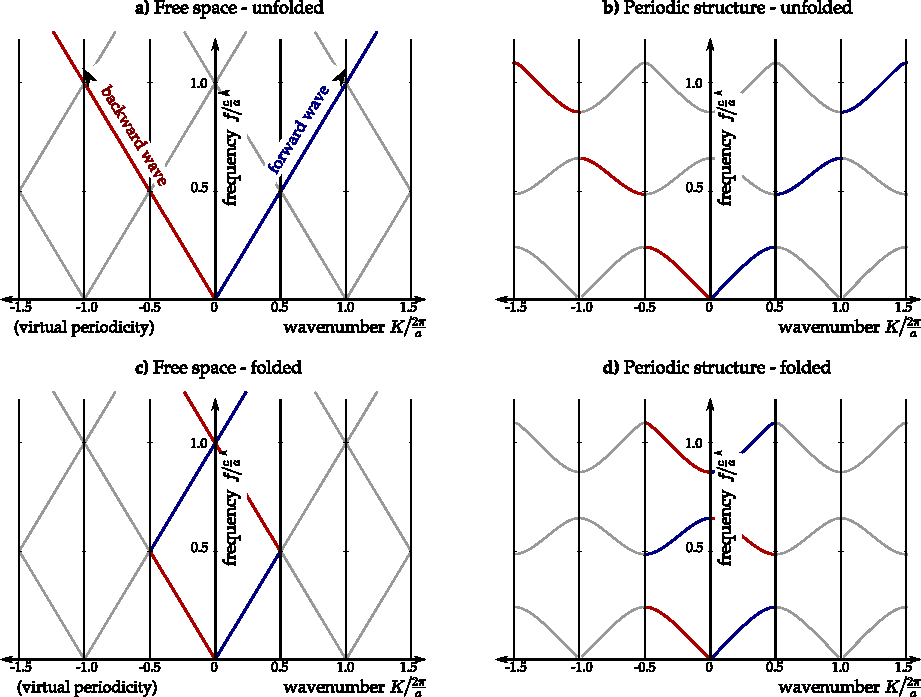
\includegraphics[width=17cm]{img/PhC_folding_illustration.pdf} 
\end{figure}
When the wavelength is less than double cell spacing, or equivalently when $2\pi c /K < 2 a$, the unit cells can scatter the forward propagating wave into the backward direction and vice versa. In an infinite periodic structure the energy transfer must be conserved, so the forward and backward waves must be of the same amplitude.\footnote{The equilibrium forward and backward wave amplitudes may, however, differ in some cases even in in infinite periodic structure. One example is when the constituent materials lose time-reversal symmetry due to static magnetic field.} We assume this also in this example with virtual periodicity. The \textit{Bloch wave} (\ref{eq_bloch}) is a product of two functions, and it gives one degree of freedom to select which part of (\ref{eq_bloch}) expresses the phase shift across one unit cell. Two different conventions are used in the literature.
\begin{enumerate}
 \item{In the \textit{unfolded} plot, the phase shift is expressed entirely by the envelope $\mathrm{e}^{\mathrm{i}Kz}$. One can always find a line coming from the front side of a unit cell to its back side, along which the mode function does not change its phase significantly $\mathbf{u(\mathbf{r})}$. In other words, the volume of the unit cell is not divided by any \textit{nodal plane} in the real part of electric field  $\mathbf{u(\mathbf{r})}$. (However, closed nodal planes within the unit cell may appear due to individual resonances.)

In vacuum, the mode function takes the simplest form, being constant $\mathbf{u(\mathbf{r})} = 1$ at all frequencies. The dispersion relation of vacuum forms a direct line as plot in Fig. \ref{fg_phc}a.} 
 \item{The \textit{folded} plot requires $K/\left(\frac{2\pi}{a}\right) \in (-\frac{1}{2}, \frac{1}{2})$ and the remaining phase is mostly expressed by the mode function. 
Further savings of space in the plot can be made using the symmetry of the forward and backward waves, so only the positive half for $K/\left(\frac{2\pi}{a}\right) \in (0, \frac{1}{2})$ has to be plot to describe the mode structure.} 
 \end{enumerate}
Although maybe less instructive, usually the \textit{folded} bands are plot in the literature and they are used also in Fig. \ref{fg_1dbd}, \ref{fg_rodh} and \ref{fg_erod_radius11} below. The same approach can be used for periodic structures, where the bands are separated by band gaps, cf. Fig. \ref{fg_phc}b and \ref{fg_phc}d.
}
%}}}
\paragraph{Dispersion curves under virtual periodicity}%{{{
The vacuum properties are obviously invariant under discrete translation by an arbitrary length $a$ along the $z$-axis, which can be considered a \textit{virtual} periodicity. 
% TODO mention the terminology "band diagram" - "dispersion curves", is there any real difference?

When the wavelength is less than double cell spacing, or equivalently when $2\pi c /K < 2 a$, the unit cells can scatter the forward propagating wave into the backward direction and vice versa. In an infinite periodic structure the energy transfer must be conserved, so the forward and backward waves must be of the same amplitude.\footnote{The equilibrium forward and backward wave amplitudes may, however, differ in some cases even in in infinite periodic structure. One example is when the constituent materials lose time-reversal symmetry due to static magnetic field.} We assume this also in this example with virtual periodicity. The \textit{Bloch wave} (\ref{eq_bloch}) is a product of two functions, and it gives one degree of freedom to select which part of (\ref{eq_bloch}) expresses the phase shift across one unit cell. Two different conventions are used in the literature.
\begin{enumerate}
 \item{In the \textit{unfolded} plot, the phase shift is expressed entirely by the envelope $\mathrm{e}^{\mathrm{i}Kz}$. One can always find a line coming from the front side of a unit cell to its back side, along which the mode function does not change its phase significantly $\mathbf{u(\rr)}$. In other words, the volume of the unit cell is not divided by any \textit{nodal plane} in the real part of electric field  $\mathbf{u(\rr)}$. (However, closed nodal planes within the unit cell may appear due to individual resonances.)

In vacuum, the mode function takes the simplest form, being constant $\mathbf{u(\rr)} = 1$ at all frequencies. The dispersion relation of vacuum forms a direct line as plotted in Fig. \ref{fg_phc}a.} 
 \item{The \textit{folded} plot requires $K/\left(\frac{2\pi}{a}\right) \in (-\frac{1}{2}, \frac{1}{2})$ and the remaining phase is mostly expressed by the mode function. 
Further savings of space in the plot can be made using the symmetry of the forward and backward waves, so only the positive half for $K/\left(\frac{2\pi}{a}\right) \in (0, \frac{1}{2})$ has to be plotted to describe the mode structure.} 
 \end{enumerate}
Although maybe less instructive, usually the \textit{folded} bands are plotted in the literature and they are used also in Fig. \ref{fg_1dbd}, \ref{fg_rodh} and \ref{fg_erod_radius11} below. The same approach can be used for periodic structures, where the bands are separated by band gaps, cf. Fig. \ref{fg_phc}b and \ref{fg_phc}d.
%}}}
\subsection{Reciprocal space, Brillouin zones and isofrequency contours}
\subsection{Group velocity, phase velocity and their signs}
%\cite{Mikki}
% -> signal velocity, Group velocity, phase velocity and their signs \cite{Mikki}, group velocity can be negative or superluminal - no problem here?
% -> "Hopping model" -- individual oscillators with frequency more-or-less dependent on boundary conditions 
%			 (Neumann ... Gamma point ... "dE/dx=0"  vs.  Dirichlet ... M-point ... "E=0")
\subsection{Antiresonances and problems with local effective parameters}

%% REF \cite{wallen2010}: Anti-resonant response of resonant inclusions
%  antiresonance "may not" come from periodicity, as it is also in random structures
%% REF \cite{alu2010}: Restoring the physical meaning of MM cosstitutive parameters

% in the following we will plot the unfolded bands instead as it seems to give clearer physical interpretation of data.
% -> TODO doplnit "PhC book": dispersní křivky atd.

\subsection{Properties of photonic band-gaps}
% -> application of PBG, todo add references; formation: \cite{laktionov2008}
% -> zero-width case, as a transition between a mode traversing from one photonic band to another
% -> concept of nodal planes (or, more precisely, surfaces)
% -> exponential wave decay with phase difference across the cell
% -> note about how Fourier transform allows no point source to radiate energy within the bandgap
% -> PhCs with metallic/metamaterial inclusios, [Monsoriu, Lina Shi and friends]
\subsection{Physics of negative phase and/or group velocity media}
% -> homogeneous media with negative group velocity
% -> refraction on the boundary 
% -> negative group velocity and power flow [Mikki]
% -> negative index media
% -> isofrequency contours in DNG


\subsection{Homogenization}
\mdf{
ref Homogenisation issues - response to our paper from OpEx
\cite{rockstuhl2008transition}
\cite{paul2011reflection}
\cite{andryieuski2012bloch}
\cite{andryieuski2010homogenization} 
\cite{simovski2007bloch}
\cite{simovski2009material}
\cite{simovski2011electromagnetic}
\cite{mortensen2010unambiguous}
}
%% "process of replacing a complex structure of subwavelength sized components with an “effective medium” with uni-
%% form properties. It is a fundamentally important notion which can be traced back to the earliest days of electro-
%% magnetic theory, to the Lorentz-Lorenz and Maxwell-Garnet effective medium models [1–3]
%			[1] J. C. M. Garnett, Phil Trans. R. Soc. A 203, 385 (1904).
%			[2] D. E. Aspnes, Thin Solid Films 89, 249 (1982).
%			[3] W. Cai and V. Shalaev, Optical Metamaterials: Fundamentals and Applications (Springer, New York, 2010).

% "Metamaterials do not bring new physical phenomena, they only force one to conscientiously review the common electrodynamics. There
% are no novel phenomena, just a novel task of homogenisation and possibly enew values of constitutive parameters"


\subsection{What are metamaterials and photonic crystals?} %{{{
\add{
%% This is after the theory of eldn in periodic media.
%% Nonresonant metamaterials (ie. in the 1st Brillouin zone, see [Kadlec2008 / Vol. 33, No. 19 / OPTICS LETTERS] and Juraj]
%% resonant metamaterials operate in the 2nd BZ (or possibly even third or higher? )
%% Think over, note the paper Dominec2014

The studies of periodic electromagnetic structures is generally divided into two classes: the \textit{photonic crystals} and \textit{metamaterials}. These types of structures are formally very similar, as they are composed of 2-D or 3-D periodic array of unit cells, and the qualitative difference can be found only after the interaction with an electromagnetic wave is known. 

%The difference is in the way how the unit cell interacts with the electromagnetic field. 
In the photonic crystal (PhC), at its frequency range of operation, the effective wavelength is similar to the cell spacing and the cells scatter the propagating wave.
The energy of the resonant field is spread relatively evenly over the majority of the unit cell volume, which results in great sensitivity of the PhC behaviour to its periodicity and typically also in a high spatial dispersion. The most prominent phenomenon observed in PhC is the emergence of forbidden photonic bands around resonant frequencies, where the light can not propagate through the structure. 

On the contrary, 
the cells of a metamaterial (MM) are expected to exhibit individual resonances which should not significantly couple to each other. 
At the resonant frequencies in the metamaterials, the majority of the energy of the electromagnetic field is localised in a fraction of the unit cell volume, so that the behaviour of the metamaterial usually has only weak spatial dispersion, if any. This allows one to describe many metamaterials with acceptable precision as a homogeneous medium with a index of refraction $N(f)$, wave impedance $Z(f)$ and related effective permittivity $\varepsilon(f)=N/Z$ and permeability $\mu(f)=NZ$. 

Both types of structures exhibit the most interesting behaviour at their frequencies of resonance, but the different types of resonances define the technology and materials used to build them. The resonances in PhC rely on wave scattering, which can be easily obtained with any ordinary low-permittivity material such as silica or silicon. On the other hand, the resonances 
%but the mentioned difference has profound consequences on the behaviour of the structure. 
%}}}

}
\begin{figure} \caption{img/mm-phc-diagram.pdf}  \centering 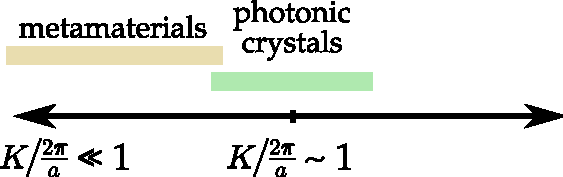
\includegraphics[width=10cm]{img/mm-phc-diagram.pdf} \end{figure} \clearpage
%% MM: HOW the light propagates.  <------>      PhC: IF the light propagates.
%% Definitions:
%% Igor Tsukerman: (Nonlocal homogenization of metamaterials by dual interpolation of fields)
%%   "metamaterials - artificial periodic structures with features smaller than the vacuum wavelength"
%% note that Veselago68 speaks about a truly *homogeneous* medium
% -> cloaking (aside from losses)
% -> superlens (aside from losses and aberration, in a hypothetical case that the MM structure can be made much finer than a detector ...)
% -> hyperlens 
%    The resolution of metamaterials is hindered by their internal cell size, and even sooner, by the spatial dispersion.
%    Hyperbolic metamaterials are commonly thought to be able to form a hyperlens, but the hyperbolic shape of the IFC is only an approximation
%    for low wavenumber; it possibly strongly differs when K~is big, and possibly also forms a closed surface instead of infinite hyperboloids.
% -> metasurfaces (impedance engineering, tunable properties, thin high-contrast filters)
% Losses are in \cite[p. 708]{born1999book}


\paragraph{Historical regards}
\paragraph{Attempt of proper definition of Metamaterials}
%% TODO
%% This is after the theory of eldn in periodic media.
%% Nonresonant metamaterials (ie. in the 1st Brillouin zone, see Juraj]
\cite{richter1995}
\cite{kadlec2008}

More detailed investigation shows that the effective-medium approach does not give accurate results when the structure is not infinite \cite{richter1995}, as is often the case. Therefore, a numerical computation using the rigorous coupled-wave analysis (RCWA) or using FDTD has to be used.

%% note Silveirinha 2007 
%% resonant metamaterials operate in the 2nd BZ (or possibly even third or higher? )
%% Think over, note the paper Dominec2014

%% PK: "The word “metamaterial” (MM) appeared first in the paper by Smith et al. in 2000 [6] where a structured material" -- is it true?

% "note that whenever a transmission is plotted, one always refers to a finite sample; in the discussion of infinite (periodic) media, 
%       only the allowed or forbidden band are to be discussed"



\section{Materials available for metamaterial construction}
\subsection{General notes}
% TODO we refer to tunability - complete it in the rest of the document!!
%% TODO unify impedance as `Z', not `z'
\subsection{Dielectrics}
\subsection{Metals}
% and oxides for optical: Naik2011.pdf
\subsection{Superconductors}
\subsection{Tunable and switchable materials}
\subsection{Specifics of the terahertz range}



%Introduction
	%What is metamaterial
	%Motivation for MM
	%Motivation for THz range
%Fundamentals
%Dielectric spectra
%eps,mu -> N,Z -> reflectivity
%K-K relations
%putting two resonances near to each other annihilates their “wings”
%→ hard to make a broadband-operating passive MM
%Metal eps spectra
%different models: Drude, lossy Drude
%spatial view of E+M wave propagation  (propagating/standing wave)
%in free space
%in arbitrary electromagnetic material 
%reflection on metal surface (PEC) and on PMC
%surface plasmons, standing/propagating
%non-lossy and lossy metal (-> quasi-bound states)
%interpreting resonance (and Fano-resonance) curves
%wave in free space → s12 ampli constant, phase constantly growing; (s11 zero)
%→  in polar plot: a clockwise rotating unit vector
%reflective surface → s11 ampli constant, phase constantly growing; (s12 zero)
%simple resonance (in SRR?) 
%→  reflectivity peak
%→  losses
%in polar plot of s12: fast clockwise curl, approaching zero point, phase up-DOWN-up
%in polar plot of s11: clockwise curl starting at zero, making trip, returning to zero
%Fano resonance: requires spiral segment of curve
%case of "little fast curl 1" on "big slow curl 2"
%if fres1 = fres2 → subtractive effect, both in amplitude and phase; phase up-down-UP-down-up
%if fres1 < fres2 → …
%find out the difference between:
%two coupled broad resonances with interaction inbetween?
%Capacitive, inductive, resistive coupling?
%a “fast” and a “slow” resonance superposed?
%Two oscillators with nearly the same frequency:
%electric+electric or magnetic+magnetic → strong coupling, leads to twice curled curve in polar plot
%electric+magnetic → weak or no coupling (magnetic dipole: H field even, Efield odd; electric dipole: H field odd, E field even → may be regarded as zero inner product of the field functions)
%Scaling and non-scaling properties [Zhou PRL 2005]
%(Mode curve anticrossing)
%Babinet principle
%(Quantum states in left-handed media?)
%
%Building metamaterials: key principles
%Homogenisation
%methods, issues, desired homogenized parameters
%Metal functions
%diluted metal → Pendry1996's low frequency plasmons
%(Are cut-wire stripes useful e.g. for stable numerical simulations? They have finite eps at freq=0)
%antennae: resonator-field coupling
%metallic resonators: negative mu from SRR/Horseshoe/double-stripe
%Bianisotropy and chirality
%SRR and double-SRR
%keeping rotational-translational symmetry
%tunability
%MM impedance and coupling to free-space waves
%Mode coupling
%capacitive/resistive, behaviour, conditions, applications
%relations between MM and photonic crystal
%Higher-order Bloch modes
%
%Selected all-dielectric metamaterials
	%Mie resonances in high-permittivity microspheres
%
%Selected metalo-dielectric metamaterials
	%Aperture-array transmission
		%Wood anomaly in slit arrays
		%Wood anomaly in hole arrays
		%Standing SPP wave
	%“thin wires [8], [28], Swiss rolls [9], SRRs [9], electric SRRs (eSRRs) [29], [30], pairs of rods [10], [12], [31], pair of crosses [32], fishnets [17], [33]”
%
%== Weird ideas to elaborate ==
%* helical wire medium -> higher inductive load -> enables low plasma freq even for thicker wires
	%---> calculate FDTD
	%---> measure   TDTS with light bulb wires!
%* Possibility of standing phonon-polariton on SiC (!) 
%* try the anisotropic magnetic goo from the drawing board for children (but for electrical response)
%* find out how they could achieve negative phase speed
%* quantum point of view to negative phase/group velocity 

% TODO: 
% Electrodynamics of continuous media
% -> Electromagnetic wave in vacuum
% -> Lorentz-Drude model
% -> Dispersion relation in Lorentz-Drude media
% -> Drude model, conductivity and superconductivity
% Spatial-dispersive model for continuous media
% -> General formulation of spatial dispersion
% -> Magnetic effects included in spatial-dispersive permittivity
% -> Comparison of eps-mu and spatial-dispersive models (electric quadrupoles..., [Merlin])
% -> Why magnetic resonances do not contribute to static permeability?
% Electrodynamics of periodic structures
% -> Bloch theorem (and its proof)
% -> K-space and isofrequency contours
% -> Group velocity, phase velocity and their signs [Mikki]
% -> Homogenisation by NRW algorithm, automatic branch selection
% -> Antiresonances -- problems with epsilon-mu approach
% -> EDB model for periodic structures
% Homogenisation algorithms 
% -> PWEM
% -> Reflection-transmission, or NRW, method
% -> Current-driven homogenisation

% Numerical methods used
% -> 


\section{Electrodynamics of continuous media} % TODO
\subsection{Electromagnetic wave in vacuum} % TODO
\paragraph{Maxwell equations} In the realm of classical physics, the electromagnetic phenomena are governed by the \textit{Maxwell equations} in the following form: %{{{
%We assume here that there are no free charges and no currents in the structure: 
\begin{equation} \nabla \cdot  \D = 0, \label{eq_me1}\end{equation}  
\begin{equation} \nabla \cdot  \B = 0, \label{eq_me2}\end{equation}  
\begin{equation} \nabla \times \E = -\frac{\partial \B} {\partial t}, \label{eq_me3}\end{equation}  
\begin{equation} \nabla \times \HH =  \frac{\partial \D} {\partial t}, \label{eq_me4}\end{equation}  
where the $\mathbf{E}$ and $\mathbf{H}$ are the electric and magnetic vector field, and $\mathbf{D}$ and $\mathbf{B}$ are the electric and magnetic induction %% FIXME
, respectively. These two pairs of field and induction are related in a similar way as a force is related to the strain. These \textit{constitutive relations} describe the medium the wave propagates in, and in vacuum they take the simplest possible form:
\begin{equation} 
\mathbf{D} = \varepsilon_0	\E, \quad\quad\quad 
\mathbf{B} = \mu_0			\HH,
\label{eq_ce}\end{equation}
the $\varepsilon_0 = 8.85\cdot10^{-12}$ F/m being the \textit{vacuum permittivity} and $\mu_0 = 1.25\cdot10^{-6}$ H/m being the \textit{vacuum permeability}. 
Pages \pageref{starttext}--\pageref{endtext} of this thesis will be concerned with computation, interpretation, and experimental verification of the Eq. (\ref{eq_me1}--\ref{eq_me4}) solutions for some particular choice of constitutive equations.
\label{starttext}
%}}}
\paragraph{Wave equation} The pair of first-order differential equations (\ref{eq_me3}, \ref{eq_me4}) can be converted to a single second-order differential equation. To this end, we apply an extra curl operator $\nabla\times$ from left, and substituting from one equation into the another, we accumulate two curl operators on the left hand side and two derivatives on the right hand side: %{{{
\begin{equation} \nabla\times (\nabla\times \E) = \nabla\times \left(- \frac{\partial \B} {\partial t}\right) = -\mu_0 \frac{\partial}{\partial t} \left(\nabla\times \HH\right) 
= -\mu_0 \frac{\partial^{2} \D}{\partial t^{2}} = -\mu_0 \varepsilon_0 \frac{\partial^{2} \E}{\partial t^{2}}.  \label{eq_elim}\end{equation}
Using the vector calculus identity
\begin{equation} \nabla\times (\nabla\times \E) \equiv \nabla (\nabla \cdot \E) - \nabla^2 \E, \label{eq_rotrot}\end{equation}
we obtain the \textit{wave equation} for the electric field: 
\begin{equation}  \nabla (\nabla \cdot \E) - \nabla^2 \E = -\mu_0 \varepsilon_0 \frac{\partial^{2} \E}{\partial t^{2}}.  \label{eq_wave}\end{equation}
%Note this holds for each component of electric field independently. -- NOT: the divergence is not independent of other components
Starting with Eq. (\ref{eq_me4}) instead of (\ref{eq_me3}), the same result and further discussion can also be easily obtained for the magnetic field.
%}}}
\paragraph{Plane wave dispersion relation in vacuum} The solutions of the wave equation (\ref{eq_wave}) are known to take the form of a plane harmonic wave in the simplest case, and in any other case the fields can be decomposed as a linear superposition of more such waves and treated separately. Using the complex notation, the field of the plane wave is defined as a function of time $t$ and position in space $\rr$:%{{{
\begin{equation} \E(t, \rr) := \E_0 e^{\ii\omega t - \ii\kk\cdot\rr} \label{eq_pw}\end{equation}
The plane wave is fully characterised by its amplitude vector $\E_0$, \textit{angular frequency} $\omega$ and \textit{wave vector} $\kk$. 
However, only some combinations of these parameters provide a physical solution of the wave equation (\ref{eq_wave}). The allowed pairs of ($\omega, \kk$) can be expressed by first substituting the differential operators by their equivalents for a particular plane wave: %TODO explain
\begin{equation} \nabla \rightarrow -\ii\kk, \quad\quad\quad 
\frac{\partial} {\partial t} \rightarrow \ii\omega, \label{eq_difftok}\end{equation}
so the wave equation (\ref{eq_wave}) for a plane wave can be modified the following way:
$$					\nabla (\nabla \cdot \E) - \nabla^2 \E				  =	-\mu_0 \varepsilon_0 \frac{\partial^{2} \E}{\partial t^{2}},  $$
$$				 -\ii\kk (-\ii\kk \cdot \E)  - (-\ii\kk \cdot -\ii\kk) \E = -\mu_0 \varepsilon_0 (\ii\omega)^2 \E, $$
\begin{equation}   - \kk (\kk \cdot \E)      +          k^2 \E            = +\mu_0 \varepsilon_0 \omega^{2} \E.  \label{eq_wavek}\end{equation}
In vacuum, the electric field and wave vector are perpendicular %% todo? PROOF?
, i.e. $(\kk \cdot \E) = 0$. Therefore, the \textit{dispersion relation} for a plane wave in vacuum is trivial:
\begin{equation} k~= \sqrt{\mu_0 \varepsilon_0}\; \omega = \frac{\omega}{c}, \label{eq_dispeq_vac}\end{equation}
where we defined the \textit{speed of light} $c := \frac{1}{\sqrt{\mu_0 \varepsilon_0}}$.
%}}}
\paragraph{Lorentz-Drude model}
The Drude model of lossy metals assumes the relative permittivity in the form
\begin{equation} \epsr(\omega) = 1 - \frac{\omega_p^{2}}{\omega^{2} + \ii\gamma\omega}, \label{eq_}\end{equation}
where $\omega_p$ and $\gamma$ are two independent constants that describe the metal.  The former is the \textit{plasma frequency} -- the frequency of collective charge density oscillation, above which the metal allows the electromagnetic wave to propagate through. The latter is the \textit{scattering frequency} which describes how often the charge carriers are scattered from their otherwise free motion, in the simplification of the Drude model. Both have the dimension of $\mathrm{rad\; s^{-1}}$. 

If $\gamma$ is nonzero, the permittivity is generally a complex function and it can be separated into its real and imaginary part $\varepsilon_r = \varepsilon_r'+\ii\varepsilon_r''$ by expanding the above fraction by its complex conjugate
\begin{equation} \varepsilon_r = 1 - \omega_p^{2} \cdot \frac{\omega^{2} - \ii \gamma \omega}{\omega^{4} + \gamma^{2} \omega^{2}} = 
		\underbrace{\left(1 - \frac{\omega_p^2}{\omega^2+\gamma^2}\right) }_{\text{real part } \varepsilon_r'}
+ \ii	\underbrace{\left(\frac{\omega_p^2\gamma}{\omega^3 + \gamma^2\omega}\right) }_{\text{imaginary part } \varepsilon_r''}.
\label{eq_}\end{equation}
%The real part $\varepsilon_r'$ indicates capacitive or inductive behaviour of the metal. The imaginary part $\varepsilon_r''$ describes losses which may arise either from 
% \underbrace{ }_{\text{}}
The low- and high-frequency limits of permittivity given by the Drude model are:
\begin{equation} \lim_{\omega \to 0} \varepsilon_r' = -\frac{\omega_p^2}{\gamma^2}, \quad \quad  
				 \lim_{\omega \to 0} (\varepsilon_r'' \cdot \omega) = \frac{\omega_p^2}{\gamma},\label{eq_}\end{equation}
\begin{equation} \lim_{\omega \to +\infty} \varepsilon_r' = 1, \quad \quad  
				 \lim_{\omega \to +\infty} (\varepsilon_r'' \cdot \omega^3) = 1. \label{eq_}\end{equation}
We can see that in the low frequency limit, the imaginary part of permittivity diverges (while its real part has a finite value). In the high frequency limit, the metal permittivity approaches that of vacuum, i.e. $1+0\ii$.

\subsection{Dispersion relation in Lorentz-Drude media} 
\paragraph{Local response of a dielectric} Assume a plane wave propagates through a medium containing (bound or free) charges. When an electric field $\E$ is applied, the response of the medium manifests in the electric induction $\D(t)$ in a way that is characteristic for the medium need to be accounted for in the constitutive equation. The response generally depends on the history of $\E(\tau)$ in previous time $\tau < t$, and is described by a convolution:
\begin{equation} \D(t) = \varepsilon_0 \E(t) + \int_{-\infty}^{t} \E(\tau) \chi_e(t-\tau) \mbox{d}\tau. \label{eq_chi_convol}\end{equation}
We expect the medium to be time-invariant, linear (independent, 
Using the Fourier transform


\paragraph{Kramers-Kronig relations}
Causality prevents the response from reacting to the future electric field, so the integration in Eq. (\ref{eq_chi_convol}) goes up to the current time only, $\tau \in (-\infty, t)$. The response of the medium to a real-valued field $\E$ must moreover be also real, no matter that the computations are often done even with complex field amplitude [Eq. (\ref{eq_pw})] for the sake of convenience. 

Thus, the basic physical laws impose relatively strict constraints to the time-domain response, which translate into another constraints for the possible shape of the response in frequency domain. The intuitive physical approach is based on that any time-domain response function can be trivially separated into its odd and even parts as $f(t) = f_{odd}(t) + f_{even}(t) \equiv -f_{odd}(-t) + f_{even}(-t) $, as shown in Fig. \ref{fg_kk}. 
\begin{figure}[h] \caption{} \label{fg_kk} \centering 
	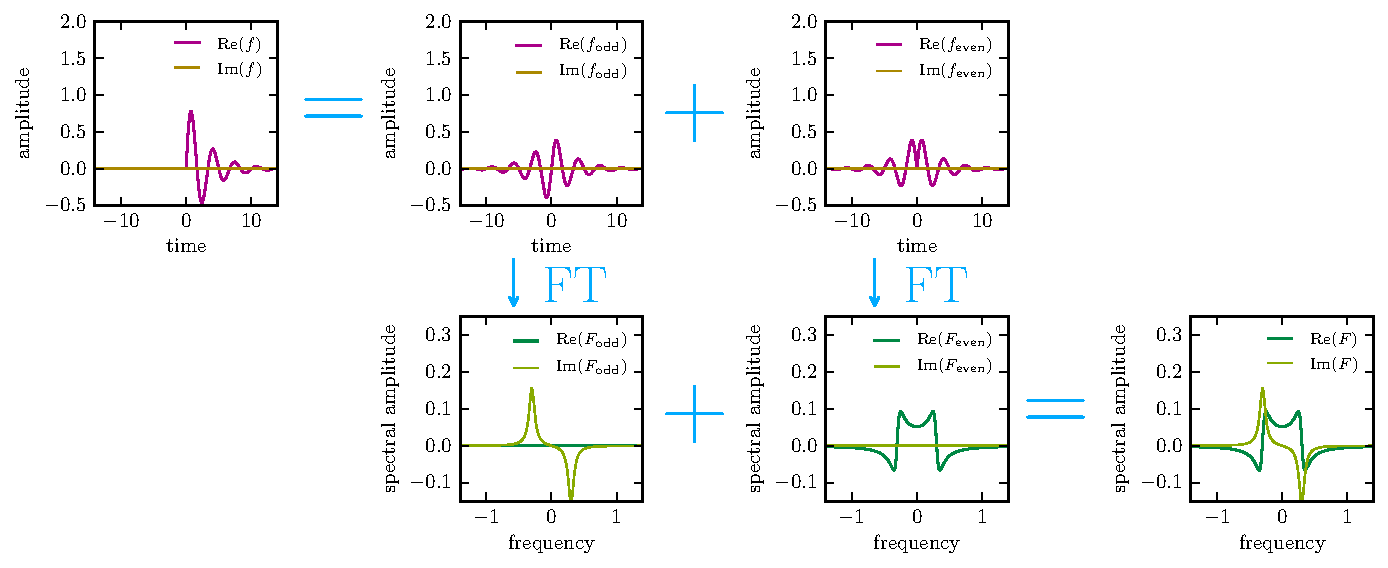
\includegraphics[width=18cm]{img/Kramers_Kronig_plot/kk.pdf}
\end{figure}

In the Fourier integral
\begin{equation} 
\begin{split} 
F(\omega)=& \int_{-\infty}^{\infty} e^{-\ii \omega t} f(t) \mbox{d}t = \\
		 =&  \frac{1}{2} \int_{0}^{\infty} e^{-\ii \omega   t } [ f_{odd}(t) + f_{even}(t)] \mbox{d}t 
		   + \frac{1}{2} \int_{0}^{\infty} e^{-\ii \omega (-t)} [-f_{odd}(t) + f_{even}(t)] \mbox{d}t  \\
		 =&  \int_{0}^{\infty} \frac{e^{-\ii \omega t}-e^{+\ii \omega t}}{2} f_{odd}(t) \mbox{d}t 
		   + \int_{0}^{\infty} \frac{e^{-\ii \omega t}-e^{+\ii \omega t}}{2} f_{odd}(t) \mbox{d}t  = 
		 =&\int_{-\infty}^{\infty} e^{-\ii \omega t} f(t) \mbox{d}t  = \\
		 =&\int_{-\infty}^{\infty} e^{-\ii \omega t} f(t) \mbox{d}t  = \\
		 =&\int_{-\infty}^{\infty} e^{-\ii \omega t} f(t) \mbox{d}t  = \\
		 =&\int_{-\infty}^{\infty} e^{-\ii \omega t} f(t) \mbox{d}t  = 
\end{split} 
\label{eq_}\end{equation}

Another, mathematical, proof can be derived from the integration in complex plane.


\paragraph{Conductivity in the Drude model}
The notion of \textit{conductivity} is widely used to describe metals and doped semiconductors i.e. media whose response to electric field is dominated by free charge carriers. Here we show that conductivity can also be expressed by the local model of permittivity, if a right frequency dependence of $\varepsilon_r(\omega)$ is chosen. For clarity, we avoid using the notion of conductivity in the rest of the thesis.

The relation between permittivity $\varepsilon_r(\omega)$ and conductivity $\sigma(\omega)$, both complex functions of angular frequency $\omega$, can be derived from the formulas for conduction and polarisation the current given as  $\rho v(t)$ excited by a harmonic oscillationg field $E(t) = \mathrm{e}^{-\ii\omega t}$, respectively: %TODO FIXME explain rho.n, use i omega t instead of -i omega t, check again...
\begin{equation} \vec \rho n(t) = \sigma(\omega) E(t) = \mathrm{e}^{-\ii\omega t}, \label{eq_rho_n1}\end{equation}
\begin{equation} \vec \rho n(t) = \frac{\partial E(t)}{\partial t} \cdot \varepsilon_r(\omega) \varepsilon_0  =-\ii \omega \mathrm{e}^{-\ii\omega t} \cdot \varepsilon_r(\omega) \varepsilon_0. \label{eq_rho_n2}\end{equation}
Both above equations describe the same quantity, so
\begin{equation} \sigma(\omega) = -\ii \omega \varepsilon_r(\omega) \varepsilon_0, \quad  \text{and} \quad  \varepsilon_r(\omega)  = \frac{\ii\sigma(\omega)}{\varepsilon_0 \omega}. \label{eq_}\end{equation}
Thus, a dielectric with real constant permittivity has imaginary conductivity, whose magnitude grows with frequency (cf. with the impedance of a capacitor). A conductor with real constant conductivity has imaginary permittivity, that diverges in the low-frequency limit. 

Using the above relation to convert metal permittivity $\varepsilon_r$ into conductivity $\sigma$ we obtain
\begin{equation} \sigma(\omega) = -\ii \omega \varepsilon_r(\omega)\varepsilon_0 = -\ii\omega \varepsilon_r'(\omega) \varepsilon_0  +  \omega \varepsilon_r'' \varepsilon_0 = 
	\ii \underbrace{\varepsilon_0 \left(-\omega + \frac{\omega_p^2\omega}{\omega^2+\gamma^2}\right)}_{\text{imaginary part } \sigma''} + 
		\underbrace{\varepsilon_0\frac{\omega_p^2\gamma}{\omega^2+\gamma^2}}_{\text{real part } \sigma'}. \label{eq_}\end{equation}
We may now express the low- and high-frequency limits also for conductivity:
\begin{equation} \lim_{\omega \to 0} \sigma' = \frac{\omega_p^2\varepsilon_0}{\gamma}, \quad \quad  
				 \lim_{\omega \to 0} (\sigma'' / \omega) = -\varepsilon_0 + \frac{\omega_p^2 \varepsilon_0}{\gamma^2} , \label{eq_}\end{equation}
\begin{equation} \lim_{\omega \to +\infty} (\sigma' \cdot \omega^2) = \varepsilon_0\omega_p^2\gamma, \quad \quad  
				 \lim_{\omega \to +\infty} (\sigma'' / \omega) = -\varepsilon_0, \label{eq_}\end{equation}
\section{The spatial-dispersive model for continuous media} % TODO
\paragraph{General formulation of spatial dispersion}
\paragraph{Magnetic effects included in spatial-dispersive permittivity}
\paragraph{Comparison of eps-mu and spatial-dispersive models}
 %(electric quadrupoles..., [Merlin])
\paragraph{Why magnetic resonances do not contribute to static permeability?}

\section{Electromagnetic waves in periodic structures}
The simplest "structure" to be started with is surely the empty vacuum with homogeneous $\varepsilon := 1$ and $\mu := 1$. One particularly simple solution of the Maxwell equations in vacuum is the planar wave propagating along the $z$-axis, defined by%{{{
\begin{equation} \mathbf{E}(z, t) := \mathbf{E}_0 \cdot e^{ikz- 2i\pi f t}, \label{eq_pw}\end{equation}
where $\mathbf{E}_0$ is the field amplitude.  This expression gives a complex function, whose imaginary part has no physical meaning and accordingly is not plot either. The following mathematical expressions however turn out to be simpler when using complex exponents instead of the purely real fields.
In a homogeneous medium, there is a simple \textit{dispersion} relation between the frequency  $f$ and the wavenumber $k$, given as
\begin{equation} f = \frac{ck}{2\pi \cdot n} = \frac{ck}{2\pi \cdot \sqrt{\varepsilon \mu}}. \label{eq_dispersion}\end{equation}
The constant $n = \sqrt{\varepsilon \mu}$ connecting the frequency and wavenumber is the index of refraction.

Let us now introduce virtual periodicity, requiring that the vacuum properties are invariant under discrete translation by an arbitrary length $a$ along the $z$-axis, which naturally holds. The important Bloch-Floquet theorem states that while the wave in periodic medium does not have to be periodic anymore, it is a product of two periodic functions:
\begin{equation} \mathbf{E}(\mathbf{r}, t) = \mathrm{e}^{\mathrm{i} Kz - 2\pi \mathrm{i} f t} \cdot \mathbf{u}(\mathbf{r}), \text{ where } \mathbf{u}(\mathbf{r}) = \mathbf{u}(\mathbf{r}+a\mathbf{z}) = \mathbf{u}(\mathbf{r}+2a\mathbf{z}) = \ldots, \label{eq_bloch}\end{equation} 
i.e. $\mathbf{u}(\mathbf{r})$ shares the periodicity with the structure and it is generally a complex vector function so it not only alters the direction and magnitude of $\mathbf E$ (or  $\mathbf H$), but also introduces \textit{phase modulation} of the wave in each cell. Note that the capital $K$ is used to distinguish the wavenumber of the Bloch wave envelope from the wavenumber $k$ in free space.

\begin{figure}[ht] \caption{Folded and unfolded dispersion curves for free space and photonic crystal. The phase difference over an unit cell can be expressed either by the wavenumber $K$ (unfolded plots \textbf{a, b} above), or it can be partially absorbed into the periodic mode function $\mathbf{u}(\mathbf{r})$ (folded plots \textbf{c, d} below) } \label{fg_phc} \centering  %% TODO write caption; complement the text to match
	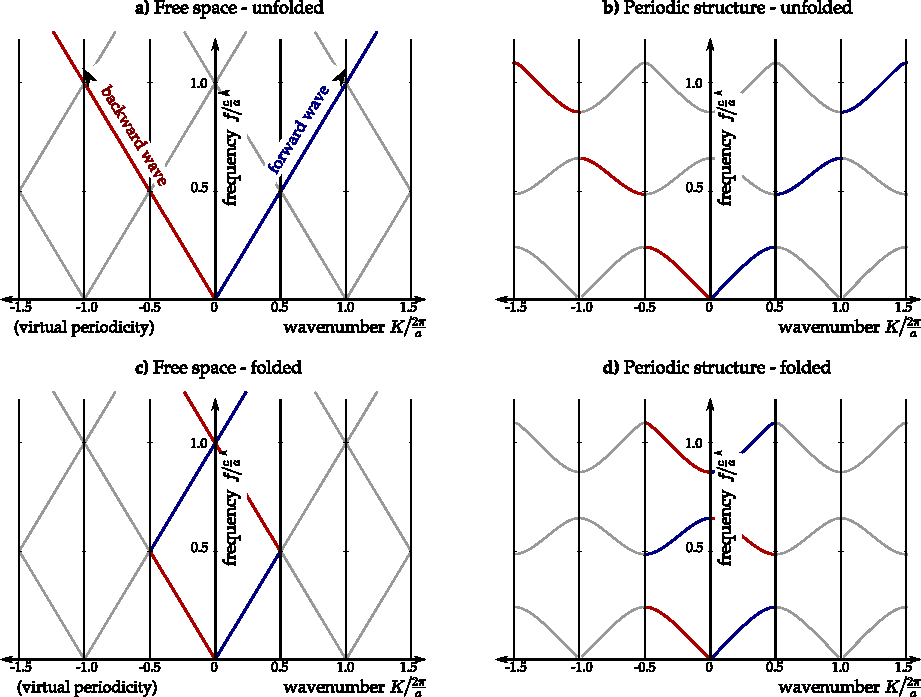
\includegraphics[width=17cm]{img/PhC_folding_illustration.pdf} 
\end{figure}
When the wavelength is less than double cell spacing, or equivalently when $2\pi c /K < 2 a$, the unit cells can scatter the forward propagating wave into the backward direction and vice versa. In an infinite periodic structure the energy transfer must be conserved, so the forward and backward waves must be of the same amplitude.\footnote{The equilibrium forward and backward wave amplitudes may, however, differ in some cases even in in infinite periodic structure. One example is when the constituent materials lose time-reversal symmetry due to static magnetic field.} We assume this also in this example with virtual periodicity. The \textit{Bloch wave} (\ref{eq_bloch}) is a product of two functions, and it gives one degree of freedom to select which part of (\ref{eq_bloch}) expresses the phase shift across one unit cell. Two different conventions are used in the literature.
\begin{enumerate}
 \item{In the \textit{unfolded} plot, the phase shift is expressed entirely by the envelope $\mathrm{e}^{\mathrm{i}Kz}$. One can always find a line coming from the front side of a unit cell to its back side, along which the mode function does not change its phase significantly $\mathbf{u(\mathbf{r})}$. In other words, the volume of the unit cell is not divided by any \textit{nodal plane} in the real part of electric field  $\mathbf{u(\mathbf{r})}$. (However, closed nodal planes within the unit cell may appear due to individual resonances.)

In vacuum, the mode function takes the simplest form, being constant $\mathbf{u(\mathbf{r})} = 1$ at all frequencies. The dispersion relation of vacuum forms a direct line as plot in Fig. \ref{fg_phc}a.} 
 \item{The \textit{folded} plot requires $K/\left(\frac{2\pi}{a}\right) \in (-\frac{1}{2}, \frac{1}{2})$ and the remaining phase is mostly expressed by the mode function. 
Further savings of space in the plot can be made using the symmetry of the forward and backward waves, so only the positive half for $K/\left(\frac{2\pi}{a}\right) \in (0, \frac{1}{2})$ has to be plot to describe the mode structure.} 
 \end{enumerate}
Although maybe less instructive, usually the \textit{folded} bands are plot in the literature and they are used also in Fig. \ref{fg_1dbd}, \ref{fg_rodh} and \ref{fg_erod_radius11} below. The same approach can be used for periodic structures, where the bands are separated by band gaps, cf. Fig. \ref{fg_phc}b and \ref{fg_phc}d.

%, but in the following we will plot the unfolded bands instead as it seems to give clearer physical interpretation of data.
%% TODO doplnit "PhC book": dispersní křivky atd.
%}}}
\section{What are metamaterials and photonic crystals?} 
%% TODO%{{{
%% This is after the theory of eldn in periodic media.
%% Nonresonant metamaterials (ie. in the 1st Brillouin zone, see [Kadlec2008 / Vol. 33, No. 19 / OPTICS LETTERS] and Juraj]
%% resonant metamaterials operate in the 2nd BZ (or possibly even third or higher? )
%% Think over, note the paper Dominec2014
%}}}

\section{Lorentz-Drude model}

% TODO Two questions: why omega_p had to be normalized by sqrt 2pi and why limit of hi-freq sigma'' had to be divided by 2pi?

\subsection{Conditions of stability in FDTD}
%TODO 
The finite-difference time-domain simulation can become unstable if 


\section{Numerical methods used}
\subsection{Finite-difference time-domain simulation}
Of the three discussed numerical methods, finite-difference time-domain simulation (FDTD) is the most versatile, but also the less efficient. It requires discretisation of the simulation volume into a one-, two- or three-dimensional grid, where each grid element holds the vectors of $\mathbf E, \mathbf H$ along with the properties of the structure ($\varepsilon, \mu$). The actual computation is based on updating the fields according to the Maxwell and constitutive equations (\ref{eq_me}, \ref{eq_ce}). The computation for each grid element is therefore a simple arithmetic operation that is easy to parallelise in multiprocessing environment. FDTD can account for realistic models of material dispersion (including losses), nonlinearity and whole range of other physical phenomena.

One downside of FDTD is in that mapping the structure into the grid introduces artifacts at edges. This may be greatly alleviated by expressing the permittivity as a tensor\cite{oskooi2009subpixel}, which effectively replaces the jagged interfaces by nearly exact polyhedra, only leaving significant error on highly \textit{curved} structures.\footnote{We used the \textit{MEEP}\cite{oskooi2010meep} program from the \textit{Ab-initio group} at MIT. It implements this feature, but in our case it mostly turned out to be better just to slightly increase resolution.}
Another issue of FDTD is hidden in the need to run the full-resolution computation in the whole volume whose largest part often consists of nothing but free space. A solution to this is called \textit{subgridding}\cite{zivanovic1991subgridding}, which defines regions with different resolution, keeping it low in the non-interesting parts of the volume. 
Both staircasing and inefficiency issues are targeted by the \textit{finite-element methods} (FEM), which approximate the structure surface with a triangular mesh and fill the volume with tetrahedra, instead of an orthogonal grid. They are particularly suitable for structures with a huge difference in the scales (e.g. where there are fine features with big spacing), at the expense of substantially more complicated computation. This was not the case of our simulations, both because of the simple geometry of the metamaterial cells studied and the technological imprecision during fabrication of the samples. For specific problems, many other methods may turn out to be superior, some of them not even requiring any grid or mesh.
% TODO? Yee cell

FDTD can also be used to obtain the field shape for a monochromatic wave with some given frequency. An intuitive way is to excite the structure for a timespan long enough with a single frequency source, and take a snapshot after all transients are gone. However, a preferable approach is to run optimisation routine, searching for a field shape\footnote{This may be viewed as eigenvector problem, where the non-hermitian linear operator are the Maxwell equations and the eigenvalue is given by the desired frequency.} for which the time-step based on Maxwell equations matches the multiplication by $e^{i\varphi}$.

From its nature, the FDTD gives the time-domain response of the given structure to a broadband excitation pulse. When we process this time evolution of fields with Fourier transform, we obtain a broad spectrum of reflected and transmitted wave a from single computation. If this is desired, FDTD is highly efficient; however if we were focused on one frequency only, the \textit{frequency-domain} methods would be preferable. 



\section{Dielectric rods perpendicular to the electric field}
% todo? analytic Mie resonance frequency? -> OBrien&Pendry2002, szabos etc
Are there also different, non-Bragg, mechanisms that can create band gaps?

We would not indeed pose this question if its answer were negative. It is closely related to the \textit{internal resonances} based on non-propagating evanescent fields in the structure. The operation of all sorts of left-handed metamaterials  relies on these resonances. We conjecture such resonances may never occur in 1-D dielectric structures, so their study requires a simulation of a 2-D or 3-D structure.
% Todo elaborate the idea of nonBragg gap <-> nonradiative fields in structure <-> permittivity/permeability resonance
% Note that in 1-D dielectric PhC, all fields are propagating, none evanesecnt
% Big question: Can one approximate a metamaterial by ENG/DNG/MNG/DPS 1-D PhC??
\begin{figure}[ht] \caption{Dispersion curves for dielectric rods aligned parallel to magnetic field. The side plots show the shape of the fields in the $(x,z)$ plane, at the frequencies of the band edges. The magnetic field is plot as color map and the electric field is represented by vectors. The rod radius was chosen to 12 \% of the period. \textbf{a)} On the left, a relatively low permittivity $\varepsilon = 12$ places the magnetic resonance above the first Bragg band gap. \textbf{b)} For high permittivity dielectric $\varepsilon = 100$, the magnetic resonance forms the first band gap. } \label{fg_rodh} \centering 
\textbf{(a)}	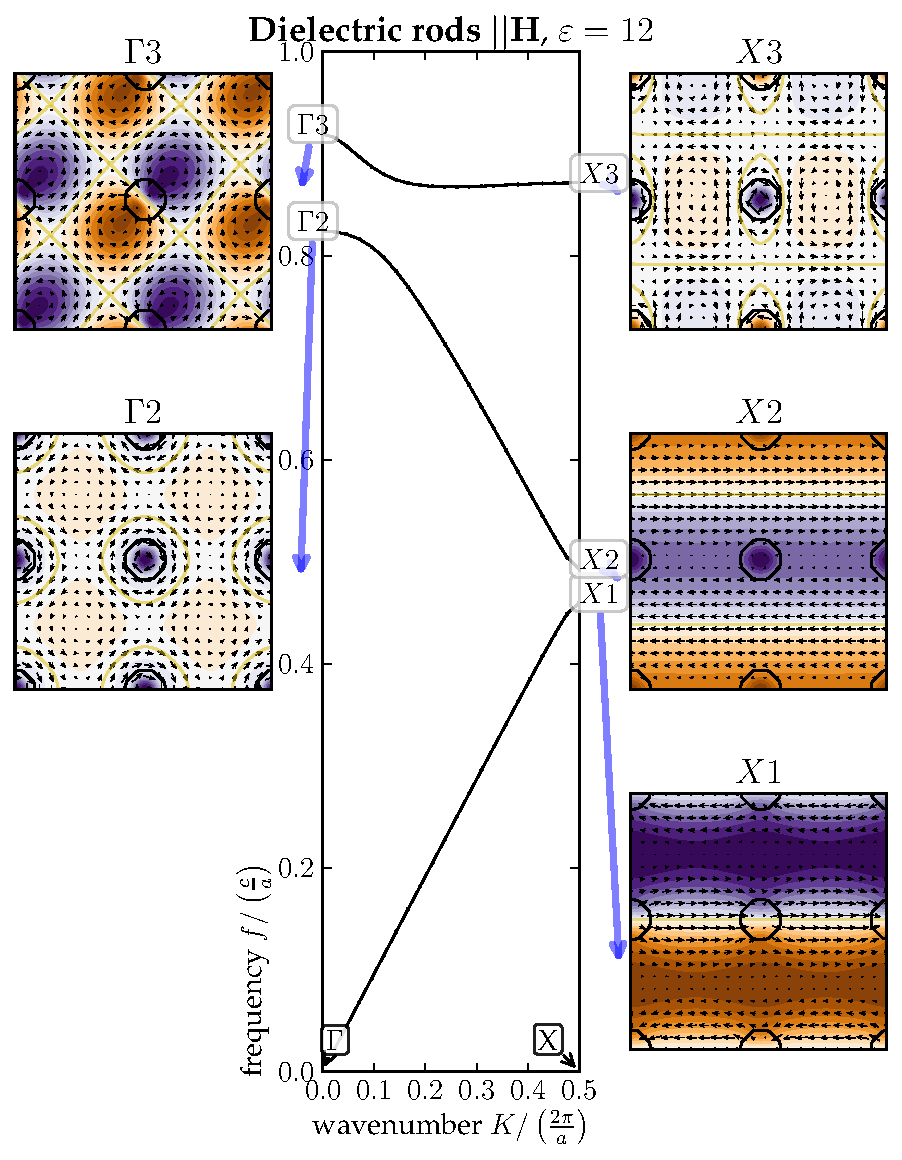
\includegraphics[width=8cm]{img/HRods_eps012_R12_PWEM.pdf}
\textbf{(b)}	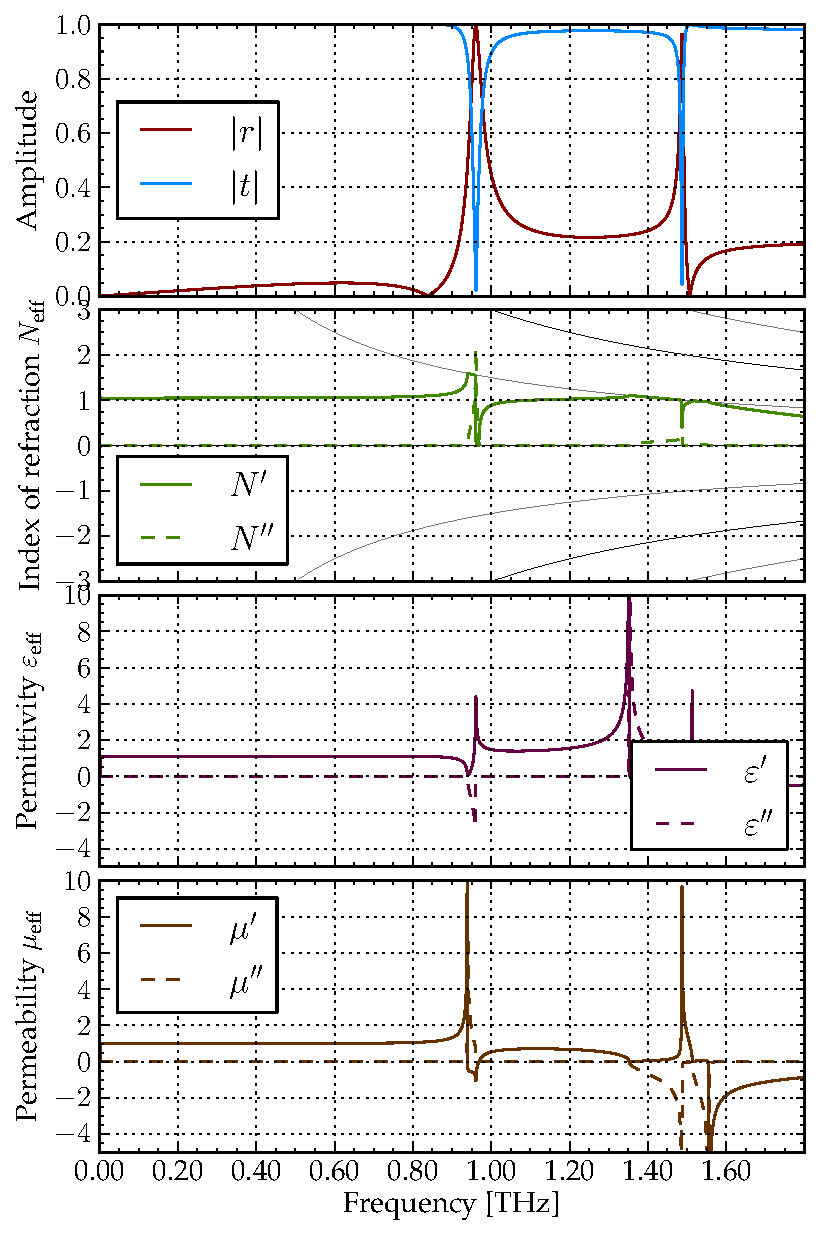
\includegraphics[width=8cm]{img/HRods_eps100_R12_FDTD.pdf}
\end{figure}

Probably the simplest example of such structures is a periodic array of high-permittivity dielectric rods, aligned parallel to the $y$-axis. (We use the convention that the structure is excited by a plane wave source with $\mathbf E || \mathbf x$, $\mathbf H || \mathbf y$ and the wave propagates along the $z$-axis). % dubious - the E, H have many directions in the unit cell; better  to write "TM"/"TE"? But this would confuse with nonperp incidence!
The inhomogeneity of the structure along the $x$-axis allows the electric field to circulate along the rod -- or, more precisely, the $\mathbf E$ field can now be decomposed into purely \textit{planar} part known from the previous section, and a purely \textit{circulating} part, that induces a magnetic flux near the rod axis. The circulating electric field is clearly visible on both plots in Fig. \ref{fg_rodh}, where all nonzero components of the fields ($H_y$, $E_x$ and $E_z$) are depicted. 

% discuss why this is not true: each lorentzian introduces delta mu -> so the low-frequency permeability of rod array should be > 1? Attracted to a magnet?
This new type of resonance is known as a \textit{magnetic Mie resonance}, \cite{obrien2002photonic, nemec2009tunable, yahiaoui2009broadband, yahiaoui2011tunable}. Unlike the Bragg gaps, it can be observed also in a single rod in free space. Being a function of the frequency of the incident wave, the magnetic dipole moment of the free-standing dielectric rod follows the characteristic Lorentzian shape of its \textit{resonance curve}. Below the resonance the magnetic dipole moment of the resonator goes to strongly positive values, while in a narrow region above the resonance it is strongly negative. How does this behaviour change if we arrange the rods in an infinite periodic array? 

%% TODO? Add the x, y, z, size scans of the ellipsoids%{{{
%> On 19 Mar 2014, at 15:57, <dominecf@fzu.cz>
%> wrote:
%>
%>> Dear Oleg and all,
%>> the frequency dependence of the Mie modes in an ellipsoid is
%>> nontrivial.
%>> Maybe some skilled mathematician could find the analytic expression,
%>> but I
%>> guess its evaluation would require a computer anyway. As an interesting
%>> numerical experiment with FDTD, I ran three scans over the X-, Y- and
%>> Z-
%>> semiaxes of a TiO2 ellipsoid, fixing the remaining semiaxes to 15 um.
%>> The
%>> ellipsoid's X-axis was oriented parallel to the electric field, the
%>> Z-axis
%>> pointed in the wave propagation direction.
%>>
%>> The results attached, best expressed by the dielectric loss spectra in
%>> bilogarithmic plot, show that the first (magnetic) mode is roughly
%>> proportional to X**(-0.4) and Z**(-0.4), while the dependence on the
%>> Y-size is even slower, similar to Y**(-0.2).
%>>
%>> The second Mie mode is more sensitive to the Z-size as Z**(-0.7), while
%>> the other sizes scale very slowly, X**(-0.15), Y**(-0.15).
%>>
%>> In all cases, the exponents of X, Y and Z~dependencies should sum up to
%>> -1, which is the obvious rule for the frequency dependence when all
%>> axes
%>> are scaled simultaneously!
%>>
%>> Note that these estimated exponents are roughly valid only near the
%>> spherical shape, ie. when X~Y~Z. As a matter of fact, the tuning curves
%>> are not straight in the log-log plots. Naturally when one ellipsoid
%>> dimension is much lower than the other two, its role becomes more
%>> pronounced.
%>>
%>> Now we are coming to the big conclusion: Near the spherical shape, the
%>> difference of exponential slope between X- and Y- elongation is
%>> (0.4-0.2)=0.2. Therefore, (15./12.)**(0.4-0.2) gives a reasonable
%>> factor
%>> of 1.0456 difference for the resonant frequencies of the magnetic mode.%}}}

The results from a PWEM computation are plot in Fig. \ref{fg_rodh}. To obtain comparable dispersion curves in Fig. \ref{fg_rodh_fdtd}, we employed the FDTD simulation and the effective parameter retrieval described above. The main differences are that in Fig. \ref{fg_rodh_fdtd} we plot the frequency $f$ on the horizontal axis and we also use the effective index of refraction $N_{\text{eff}} := K\cdot \frac{c}{2\pi\,f}$ instead of the wavenumber $K$. One advantage of this representation is that $N_{\text{eff}}$ should be compliant with the Kramers-Kronig relations. This criterion always gives \textit{only one} correct solution on how to unfold $K$ to obtain realistic $N_{\text{eff}}$. 
In the simulation, the rod spacing (or, lattice constant) $a$ was 100 \um, so the normalised frequency unit is $c/a = 3$ THz. The frequency range from 0 to 1.8 THz was therefore chosen the same as in Fig. \ref{fg_rodh}b. 
Note the first resonance shows pronounced resonant shape in the plot of permeability, which is typical of magnetic Mie resonances. In a very narrow region 960-970 GHz, the permeability $\mu_{\text{eff}}$ is real and negative. 
Apart from $N_{\text{eff}}$, the FDTD computation gives also the effective wave impedance $Z_{\text{eff}}$, which is a complementary information we need to compute the effective permittivity $\varepsilon_{\text{eff}}$ and the effective permeability $\mu_{\text{eff}}$:

\begin{equation} \varepsilon_{\text{eff}} = N_{\text{eff}}/Z_{\text{eff}}, \quad\quad\quad\quad \mu_{\text{eff}} = N_{\text{eff}}\cdot Z_{\text{eff}}.
\label{eq_epsmu}\end{equation}

\begin{figure}[ht]  \caption{Effective parameters of an array of dielectric rods $||\mathbf H$ with same parameters as in Fig. \ref{fg_rodh}b (i.e. radius of  12 \% of the period and permittivity $\varepsilon = 100$). Complex reflection $r$ and transmission $t$ spectra allow to compute the effective index of refraction, impedance (not shown), permittivity and permeability. Thin grey lines indicate the Brillouin zone boundaries.}
\label{fg_rodh_fdtd} \centering 
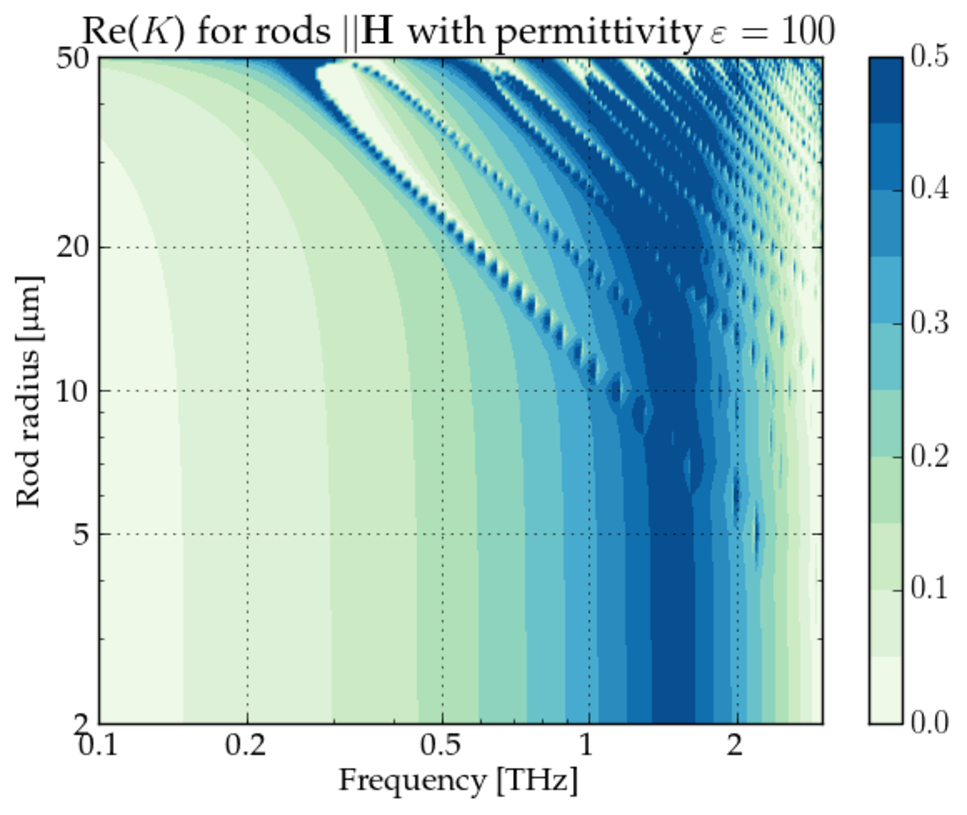
\includegraphics[width=8cm]{img/HRods_eps100_radiusscan.pdf}
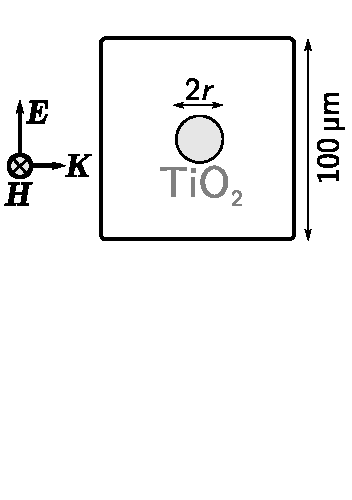
\includegraphics[width=4.5cm]{img/HRods_sketch.pdf}
\end{figure}

Other Mie resonances are located at higher frequencies. As a general rule for similar structures, the odd-numbered resonances have magnetic dipole moment (along the rod axis), whereas the even-numbered resonances have electric dipole moment (perpendicular to the rod axis). The reason is that electric dipole moments in odd resonances are suppressed due to antisymmetric shape of the mode; naturally the same holds for the magnetic moments in the even resonances.

The frequency of the Mie resonances is not significantly influenced by the photonic bands. Therefore, in order to understand the resulting band structure and its dependence on parameters, one has to disentangle which band gaps are due to Bragg reflection and which correspond to magnetic or electric Mie resonances. This is much easier knowing the spectra of $\varepsilon_{\text{eff}}$ and $\mu_{\text{eff}}$, as provided by FDTD in Fig. \ref{fg_rodh_fdtd}.
\begin{figure}[ht] \caption{The spectra of the wavenumber $K$ for different rod radii and two different rod permittivities. The wavenumber plot is folded so it ranges from 0 to 0.5, where $K\approx 0$ and $K\approx 0.5$ correspond to band gaps. \textbf{a)} Medium-permittivity rods with $\varepsilon = 12$, \textbf{b)} high-permittivity rods with $\varepsilon = 100$.  } \label{fg_hbar_radiusscan} \centering 
\textbf{a)}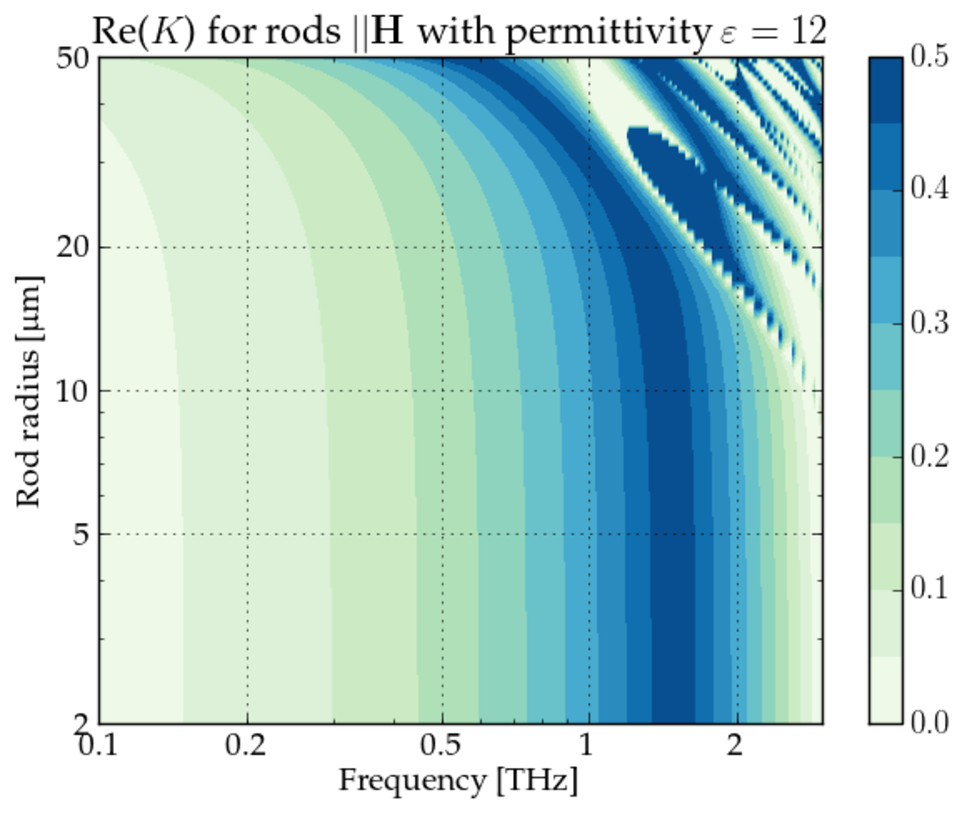
\includegraphics[width=8cm]{img/HRods_eps012_radiusscan.pdf}
\textbf{b)}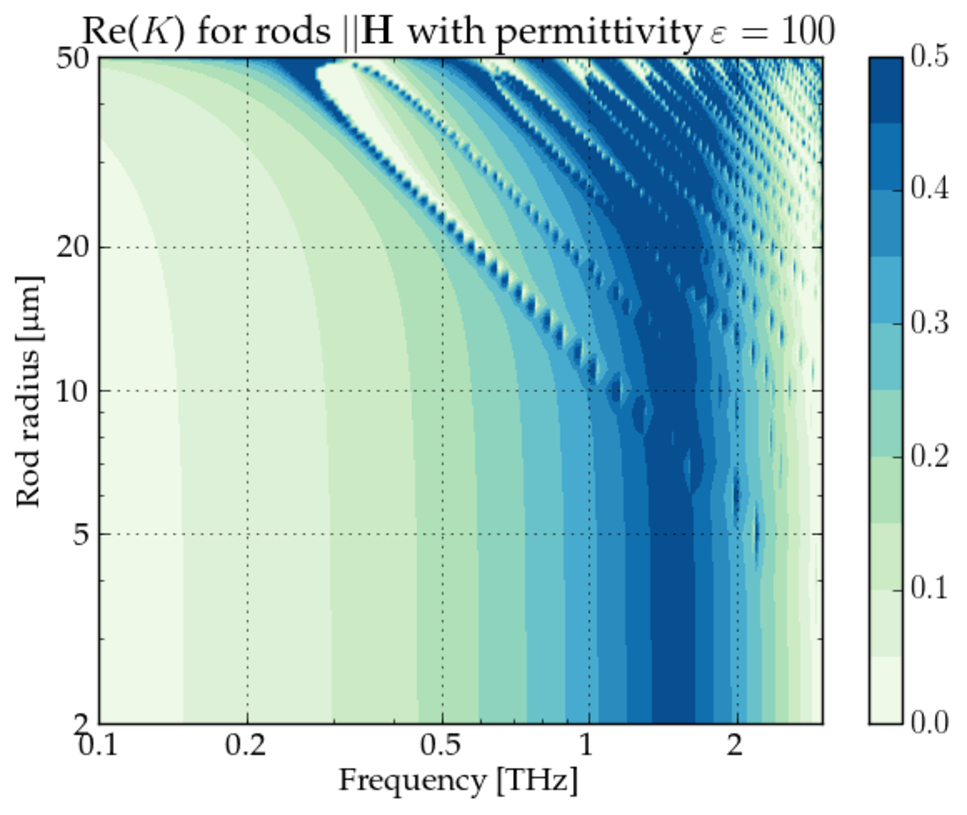
\includegraphics[width=8cm]{img/HRods_eps100_radiusscan.pdf}
\end{figure}

The photonic crystals composed of square lattice of dielectric rods have been examinated thoroughly since early 90s \cite{plihal1991two, pendry1992_transfer_matrix}. The permittivity of the constituent materials was rather low, corresponding to the optical or near-infrared frequencies, where the suitable materials usually have permittivity $\varepsilon < 12$. By parametric scans we could prove that for rod permittivity below 60 or even 80, the individual resonance is always located at higher frequency than the Bragg gap. Little, if any, attention was therefore paid to different nature of the higher resonances and most publications focused on properties and applications of the Bragg band gap.

The situation is different in the terahertz range, as the lattice of the crystalline solids often exhibits optical phonons at frequencies between 5 and 20 THz. The permittivity of many materials turns out to be much higher for frequencies below these resonances. This enables to conceive structures composed e.g. of titanium dioxide \cite{baumard1977_epsilon_TiO2} with $\varepsilon^{\text{THz}} \approx 92$ or of ferroelectrics with $\varepsilon^{\text{THz}}$ even orders of magnitude higher \cite{skoromets2011tuning}. The price to be paid for this advantage in the THz range are the relatively high losses caused by the lattice vibrations.


\begin{figure}[ht] \caption{Behaviour of the rods $||\mathbf E$, with permittivity $\varepsilon = 100$ and radius $r=11\;\upmu$m.\\
\textbf{a)} Band diagram and modes from PWEM. 
\textbf{b)} The effective parameters computed using FDTD confirm the previous results.  } \label{fg_erod_radius11} \centering 
\textbf{a)}	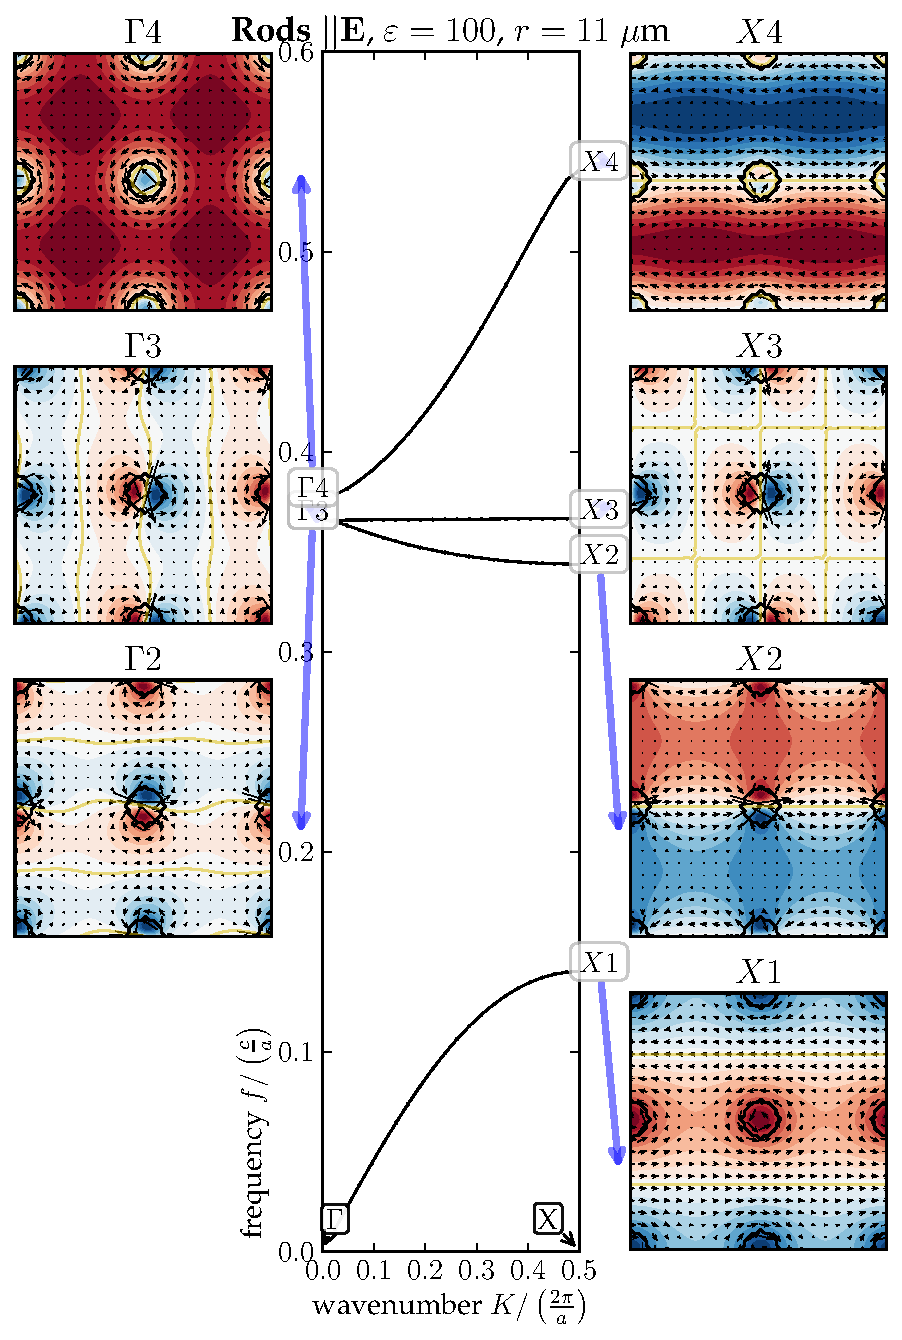
\includegraphics[width=8.5cm]{img/ERods_eps100_R11_PWEM.pdf}
\textbf{b)}	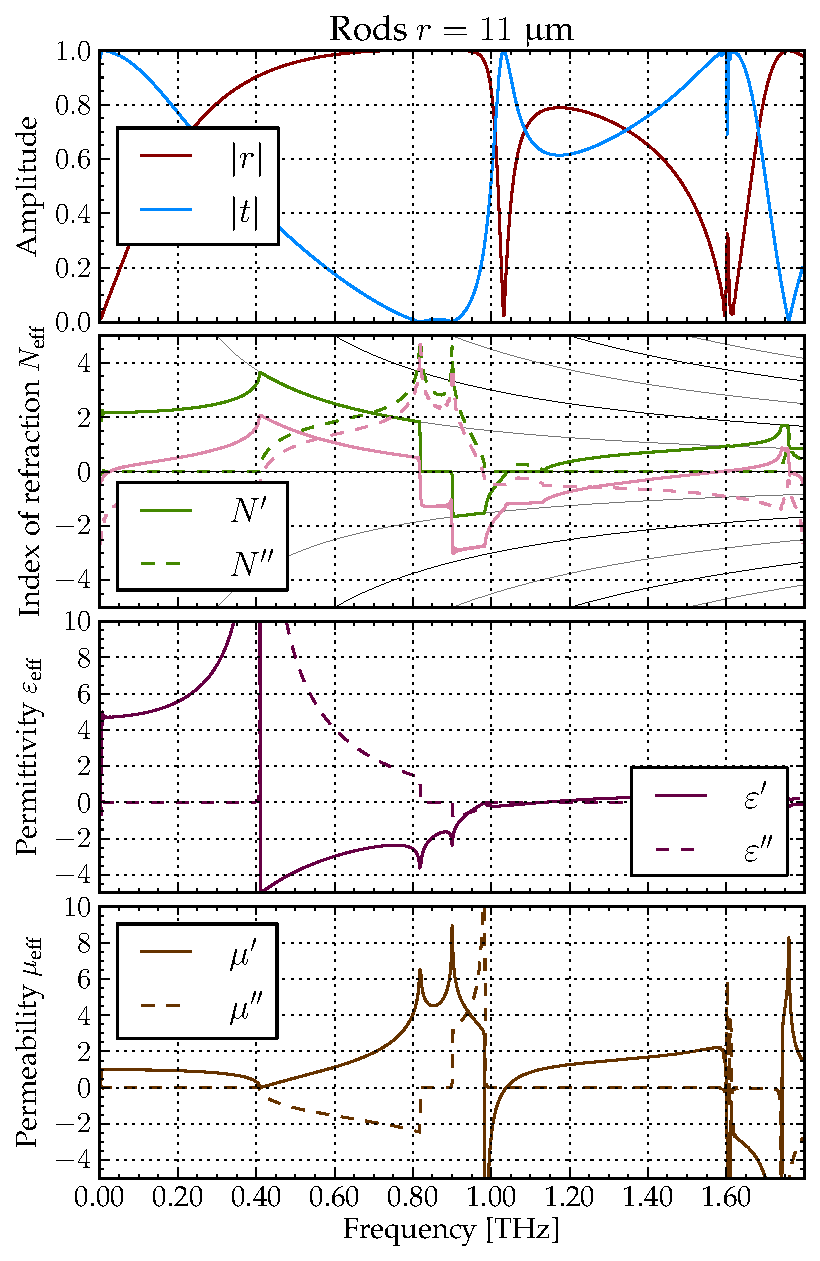
\includegraphics[width=8.0cm]{img/ERods_eps100_11um_FDTD.pdf}
\end{figure}

\section{Dielectric rods parallel to electric field}
\begin{figure}[ht] \caption{The spectra of the wavenumber $K$ for different rod radii and two different rod permittivities, analogical to Fig. \ref{fg_hbar_radiusscan} except for different orientation. \textbf{a)} Medium-permittivity rods with $\varepsilon = 12$, \textbf{b)} high-permittivity rods with $\varepsilon = 100$.  } \label{fg_ebar_radiusscan} \centering 
\textbf{a)}	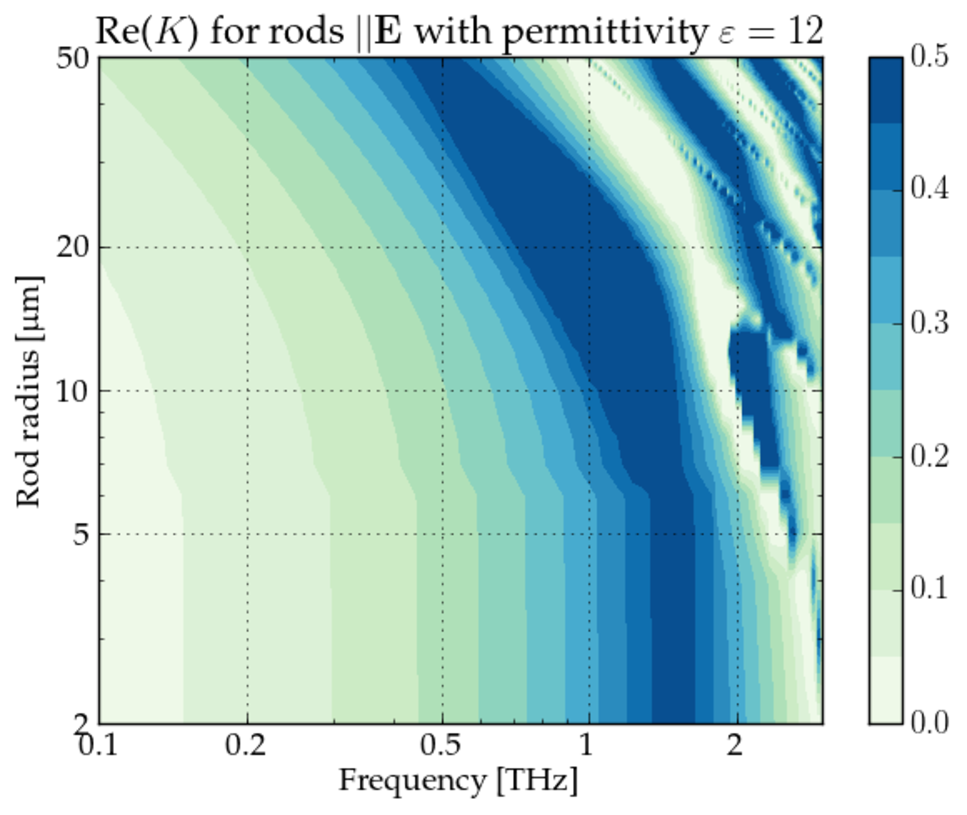
\includegraphics[width=8cm]{img/ERods_eps012_radiusscan.pdf}
\textbf{b)}	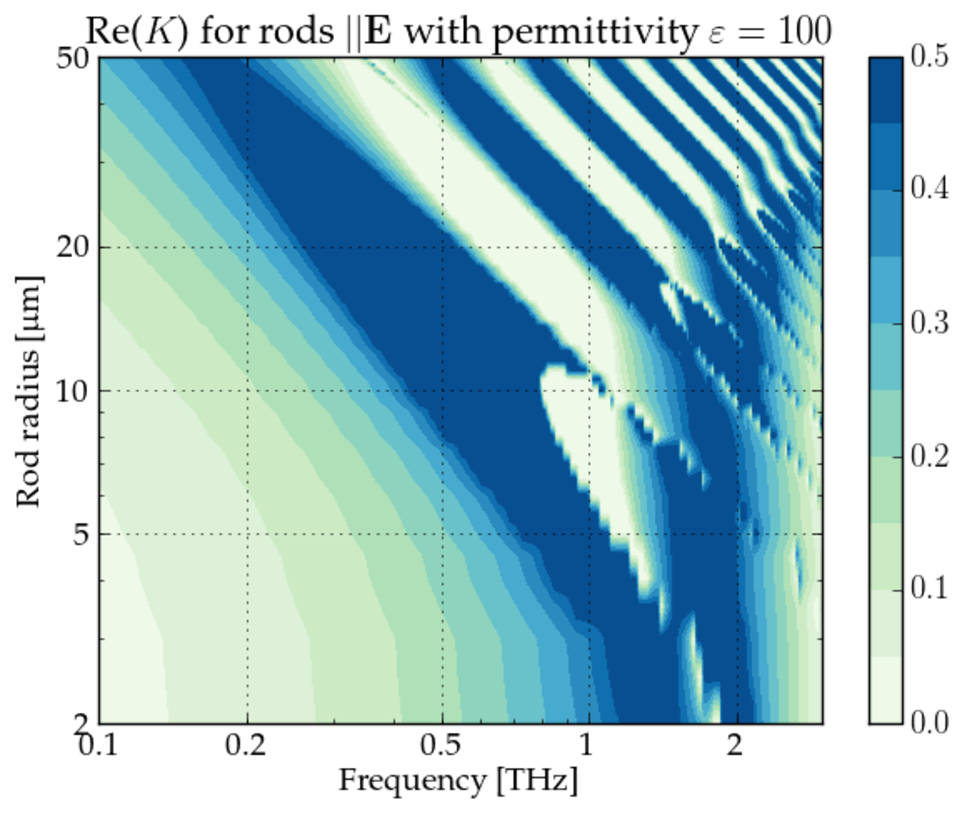
\includegraphics[width=8cm]{img/ERods_eps100_radiusscan.pdf}
\end{figure}


\begin{figure}[ht] \caption{Experimental and numerical data for strontium titanate bars $||\mathbf E$ of rectangular cross-section $26 \times 66\;\upmu$m. }\label{fg_ebars_exp} \centering 
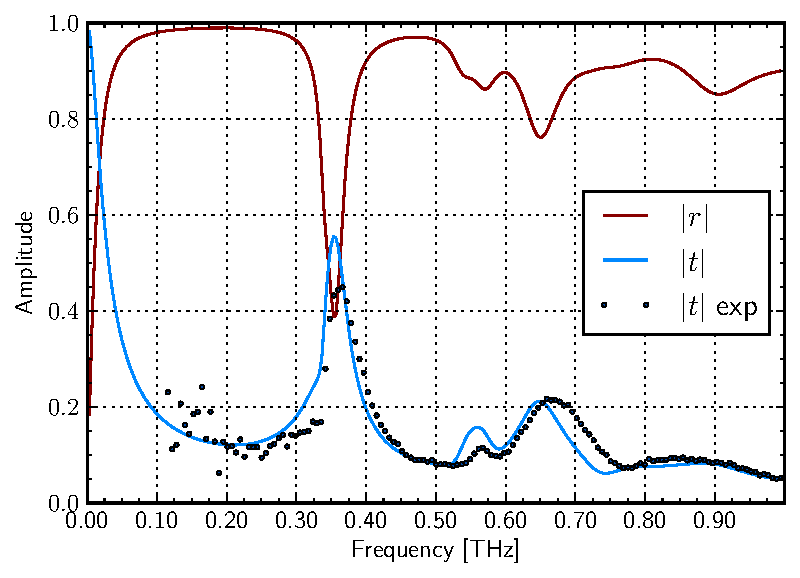
\includegraphics[width=11cm]{img/STObar_rt.pdf} 
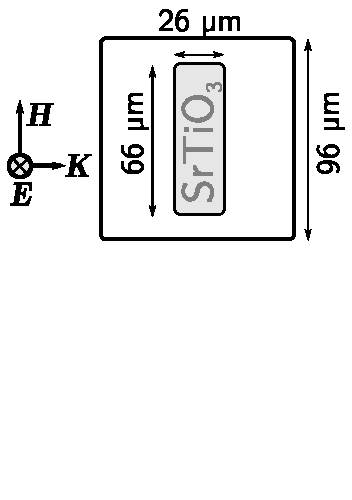
\includegraphics[width=4cm]{img/EBars_STO_sketch.pdf}
\end{figure}
% XRectWire_resolution=2.00e-06_comment=STO_simtime=1.50e-10_yspacing=9.60e-05_epsilon=6.00e+02_cells=1.00e+00_padding=5.00e-05_width=6.40e-05_monzd=1.00e-04_thick=2.60e-05_Kx=0.00e+00_Ky=0.00e+00
The dielectric bars parallel to the electric field represent the same structure as previously discussed, except that it is orthogonally rotated. There is however a qualitative difference in that the high-permittivity dielectric is continuous along the direction of the electric field, so the effect of the dielectric is expected to be much stronger. This results in that the first Mie resonance is the \textit{electric} one. Its overlap with the next magnetic resonance can eventually lead to negative index of refraction in such a structure \cite{peng2007, vynck2009}. If the permittivity of the rods is chosen to be $\varepsilon = 100$ and the periodicity of the lattice $a = 100\;\upmu$m, the negative index of refraction occurs in a narrow range of radii from 9 to 12 $\upmu$m. The behaviour of this structure with the desired radius is depicted in Fig. \ref{fg_erod_radius11}a,b.

In order to form a photonic band with a negative index of refraction, both the permittivity and permeability need to be negative. In the structure discussed, this is made possible by the frequencies of the electric and magnetic Mie resonances being close enough to overlap.
The electric resonance would be surrounded by its broad band gap between the frequencies spanning from $0.13 \cdot\frac{c}{100\;\upmu\text{m}} \approx 400$ GHz to  $0.38 \cdot\frac{c}{100\;\upmu\text{m}} \approx 1140$ GHz. This is also confirmed by Fig. \ref{fg_erod_radius11}a where the mode shapes X1 and $\Gamma$4 perfectly correspond to the electric Mie resonance. 

For the interesting range of radii around 11 $\upmu$m, the magnetic resonance introduces a new, narrow photonic band starting from X2. Now, moving on to the right plot of Fig. \ref{fg_erod_radius11}b, we can clearly identify the resonant frequencies of 815 and 900 GHz. They cause abrupt skips of the refractive index which always shift the index of refraction by one Brillouin zone down.\footnote{The individual resonance appears to be the only mechanism that causes $N'_{\text{eff}}$ to \textit{decrease} in the spectrum. In photonic bands, no matter if $N_{\text{eff}} > 0$  or $N_{\text{eff}} < 0$, the real part of $N_{\text{eff}}$ always grows in accordance with the Foster theorem. This is confirmed by the FDTD results and by their compliance to Kramers-Kronig relations. To illustrate this, the Hilbert transform of the refractive index is plot as the thin pink line and it nearly perfectly follows the green curve over whole spectrum, except for an additive constant. There is  only one acceptable physical solution that is compatible with the Kramers-Kronig relations.}
The resonance is accompanied by a sharp peak in the imaginary part of refractive index $N''$ and by transmission amplitude touching zero ($|t| = 0$). As both Mie resonances precede the Bragg gap, the index of refraction is pushed into negative values and the following photonic band gap $N' < 0$.

For completeness we add the FDTD results with effective permittivity and permeability, computed for the entire spectrum. These quantities however seem to have a useful physical interpretation only within the photonic bands, or within those parts of the photonic band gaps where $N = 0$. 
\\

The dispersion curves of the rods with radii different than 11 $\upmu$m are compared in Fig. \ref{fg_ebar_radiusscan}b based on multiple FDTD simulations. The individual resonances are again easy to be distinguished by abrupt changes from white to blue or vice versa (i.e. skips between the Brillouin zones). We can see that for radii below 8 $\upmu$m the magnetic resonance is at too high frequencies, forming its separate band gap. For even thinner rods at the very bottom edge of the plot, no individual resonance intersects with the first Bragg  band gap at all. 

An interesting qualitative change of the structure response occurs when the rods get slightly thicker than discussed above, say $r > 12\;\upmu$m. The electric and magnetic resonance frequencies do never cross over, but instead they  and an ordinary Bragg band gap remains. The transmission curve of single cell (Fig. \ref{fg_erod_radius11}) continuously shifts up and does not touch zero anymore. We may conclude that for rod radius being too high, the structure no more exhibits the negative index of refraction and starts to behave similar to the 1-D photonic crystal discussed above.
% TODO explanation by nodal planes

%The dependence of the folded wavenumber $\text{Re}(K)$ for high-permittivity rods $||\mathbf E$ is plot in Fig. \ref{fg_ebar_radiusscan}b. Starting from very thin rods ($r=2$ \um) at the very bottom of the plot, we can see the first band gap (1.3 to 1.5 THz) denoted by darkest blue is purely of the Bragg type, followed by a 

Comparing the low-permittivity and high-permittivity cases in Fig. \ref{fg_ebar_radiusscan}a,b, one can see there exists some minimum limit for the permittivity contrast that is necessary for both electric and magnetic resonances to be located in the first gap simultaneously. We determined this scale-invariant value to be roughly 80.

As a little verification that the numerical computations give sound results, we attach experimental transmission measurement of the rod array in Fig. \ref{fg_ebars_exp}.
The bars used had rectangular cross-section, being 26 $\upmu$m thick, 66 $\upmu$m  wide and their periodicity along the $y$-axis was 96 $\upmu$m.  The experimental data (points) are compared to FDTD simulation data of an identical structure (lines). The material used was strontium titanate, best matched by simulation where the permittivity was set to $\varepsilon^{\text{(1 THz)}} = 365 + 62i$.  While this structure can not provide the negative index of refraction and has very high losses, it can act as a temperature-tunable filter. The transmission peaks can be clearly identified with resonant modes and it was observed that the frequencies of the modes shift with different slope depending on parameters.  
 



\section{Dielectric spheres}
Dielectric spheres are delimited in all three dimensions, but they have much in common with the dielectric rods. Their behaviour is closer to that of the rods with orientation parallel to the \textit{magnetic field}. The reason is that the lowest-frequency resonance of both structures is generally the magnetic one, whose circulating electric field is localised in the high-permittivity volume of the particle. Higher resonances require a significant part of the electric field to pass through surrounding air.

\begin{figure}[ht]  \caption{Effective parameters of an array of dielectric spheres \textbf{a)} Ti$\,$O$_{2}$ spheres of diameter $r=25\;\upmu$m, \textbf{b)} The same Ti$\,$O$_{2}$ spheres interlaced with thin wire mesh }
\label{fg_spheres_fdtd} \centering 
\textbf{a)}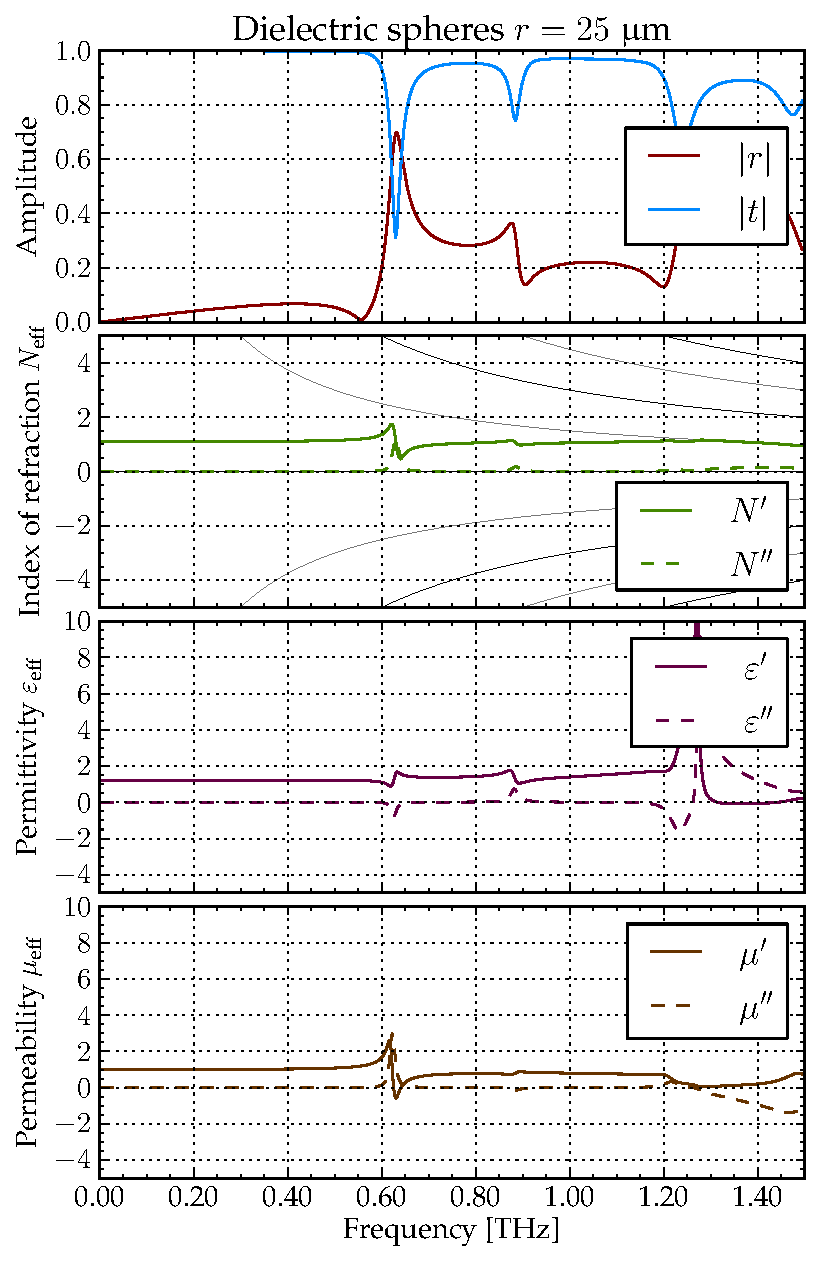
\includegraphics[width=8cm]{img/Sphere_eps100_R25_FDTD.pdf}
\textbf{b)}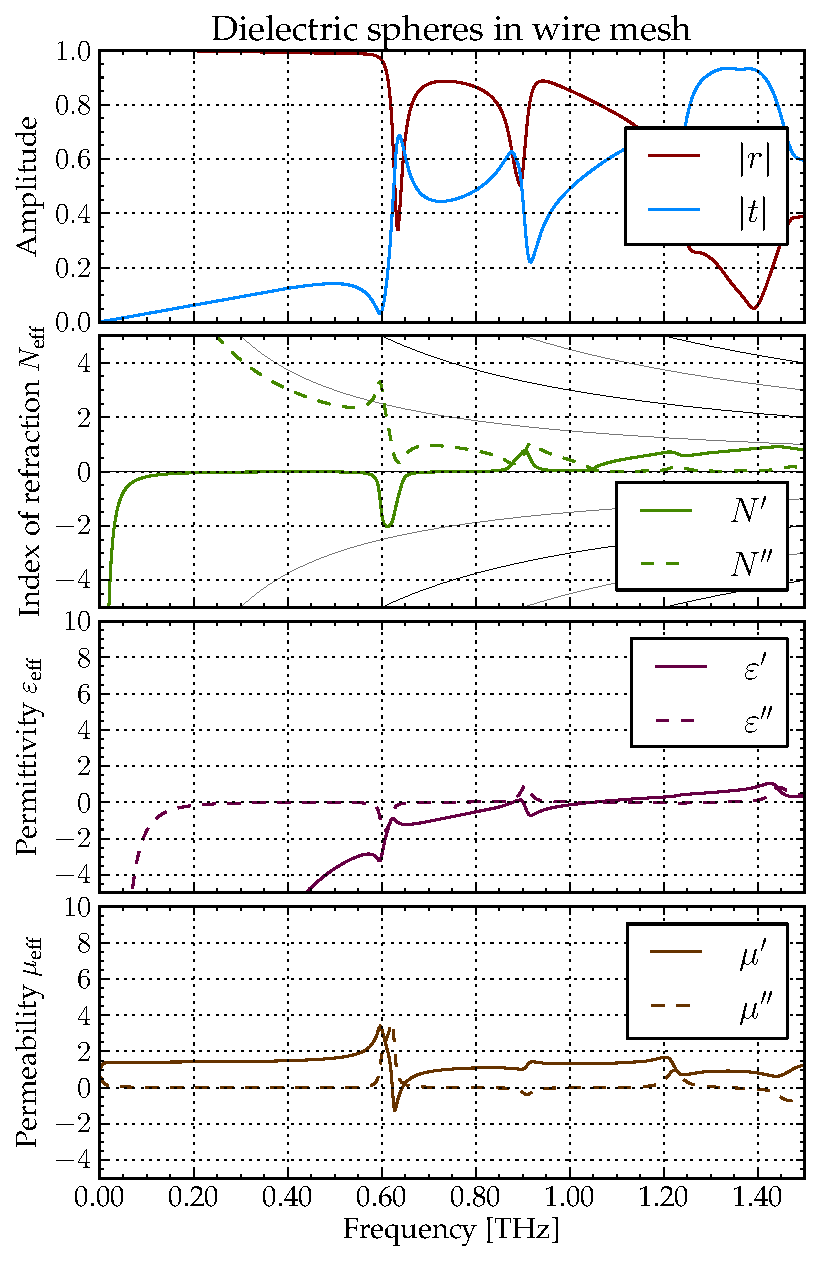
\includegraphics[width=8cm]{img/SphereWire_eps100_R25_FDTD.pdf}
\end{figure}
In contrast with previous treatment, we used a realistic model \cite{baumard1977_epsilon_TiO2} of rutile (TiO$_{2}$) for the FDTD simulations presented here to illustrate the effect of losses. The permittivity of the spheres was $\varepsilon^{\text{(1 THz)}} = 94.2+2.43\text{i}$, their diameter was set to $r=25\;\upmu$m  and their spacing along each axis was $a =100$ $\upmu$m. The resulting spectra of reflection, transmission and effective parameters are in Fig. \ref{fg_spheres_fdtd}a. A strong magnetic resonance is apparent at 330 GHz, followed by a weaker electric one at 480 GHz and another magnetic one at 670 GHz. Further resonances are gradually less visible due to lower dipole moment and also due to dielectric losses that increase with frequency. 
For completeness, we extend the frequency axis near $a/(2c) \approx 1.5$ THz, where the first Brillouin zone is reached and a classical Bragg band gap is formed.
The main difference compared to the lossless resonances discussed above (cf. Fig.~\ref{fg_rodh_fdtd}) is the continuous index of refraction, that prevents the index of refraction $N'$ near individual resonances to reach the Brillouin zone boundaries and to form clear edges of the bands. As a result, all effective parameters are continuous even near resonances and do not form separate branches.

An important property of the periodic sphere array is its \textit{isotropic} electromagnetic behaviour. It trivially follows from symmetry under any orthogonal rotation, and it also holds almost exactly under any other orientation (unless the spheres are not touching or too high frequencies are studied).

The right plot in Fig. \ref{fg_spheres_fdtd}b shows simulation results for the sphere array interlaced with a wire mesh. The wires are directed along the $x$-axis and $y$-axis, the latter orientation being included only to maintain isotropy of the structure. The wires along the $x$-axis, i.e. parallel to the electric field, have a great impact on the spectra. Most importantly, the structure is now highly reflective at low frequencies, and the resonances introduce transmission windows. (Note the previously discussed sphere array acted in opposite way!) The explanation is contained in the effective permittivity plot, where the wires introduce a region of $\varepsilon_{\text{eff}} < 0$  ranging from 0 to ca 900 GHz. More detailed study of this phenomenon is in the following section.

The magnetic resonance introduces narrow regions where $\mu_{\text{eff}} < 0$, thus leading to $N'_{\text{eff}} < 0$ and a propagation mode would occur \cite{dominec2013resonant}. The electric resonance can, on the other hand, overpower the effect of wires so that $\varepsilon_{\text{eff}} > 0$, forming a narrow band with $N'_{\text{eff}} > 0$.
%In practice the resonances are highly lossy, so only the first magnetic resonance introduces a band where the wave can propagate through several cells without being too damped. 

We performed series of experiments to measure the effective permeability  $\mu_{\text{eff}}$ spectrum in a real sample with mean sphere radius of ca. $42\;\upmu$m. The statistical deviation of the resonators size $\sigma \approx 5\;\upmu$m in the sample was unfortunately relatively broad, as was determined by means of microscopy and digital image processing. In contrast to simulations, we were able to constraint the spheres' positions to a plane only, while arranging them in a square array appeared unrealistic. We could anyway compute the single-cell permeability spectra (i. e. the yellow curve in Fig. \ref{fg_experimentalConv}) for many different resonator sizes and add them up. The resulting weighted average (blue curve) then matches the experimental data (red dots) nearly exactly. It shall be however noted that the averaged real part of $\mu_{\text{eff}}$ remained positive even with the best sieving results obtained so far.
\begin{figure}[ht]  \caption{Comparison of the effective permeability of ideal monodisperse sphere array (yellow), weighted average according to the size distribution (blue) and experimental data (red dots).}
\label{fg_experimentalConv} \centering 
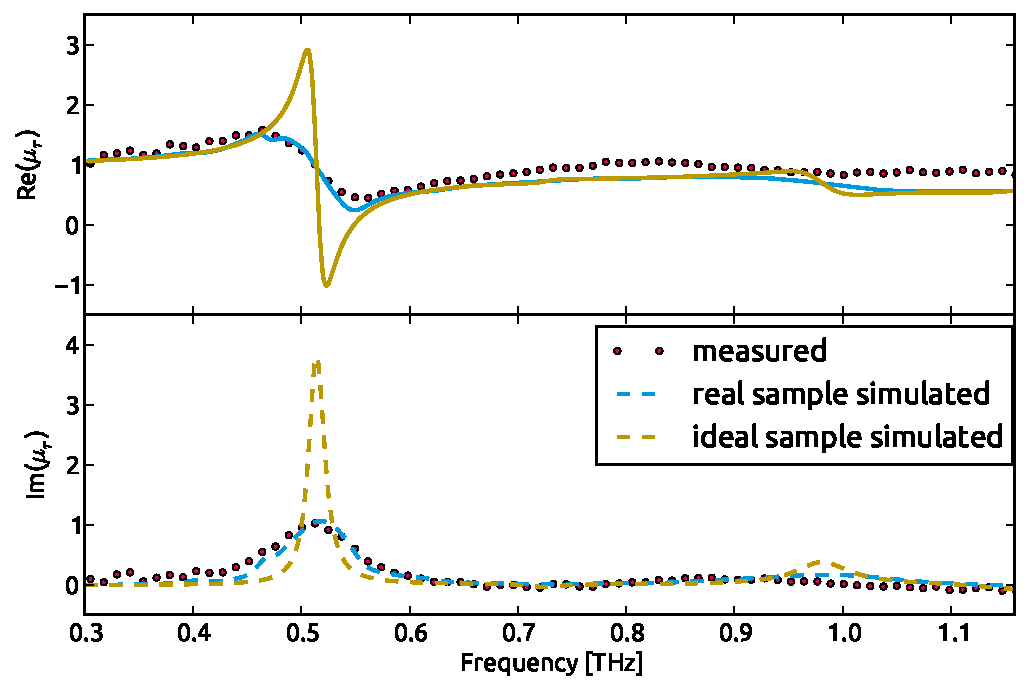
\includegraphics[width=12cm]{img/Spheres_FDTD_experimentalConv.pdf}
\end{figure}



\section{Metallic wires along the electric field: plasma-like behaviour}
A dense array of thin, perfectly conductive (PEC) wires oriented along the electric field is somewhat similar to the dielectric rods of the same orientation. It might be incorrectly expected that such an array would reflect all incident radiation, i.e. it would behave just as a metallic sheet or bulk metallic block does. The simulation proves that this expectation is wrong, even when the wire density is order of magnitude higher than that would allow diffraction. The wire array allows a part of the radiation to pass through -- in other words, no wire polarizer is 100 \% perfect no matter how conductive the constituent material is.
\begin{figure}[ht]  \caption{Effective parameters of wire mesh, wires oriented both along the electric and magnetic field, with radius of $r_w = 12\;\mu$m. A realistic Drude model was used for the metal.\\ Due to high conductivity of the wires, a wrong sign of $N'$ at 0--200 GHz and of $N''$ at 1620--2080 GHz was given by computation.\\As an illustration of the plasma-like behaviour, a grey curve shows the permittivity predicted by Drude model with $f_p = 1110$ GHz.}
\label{fg_wire_fdtd} \centering 
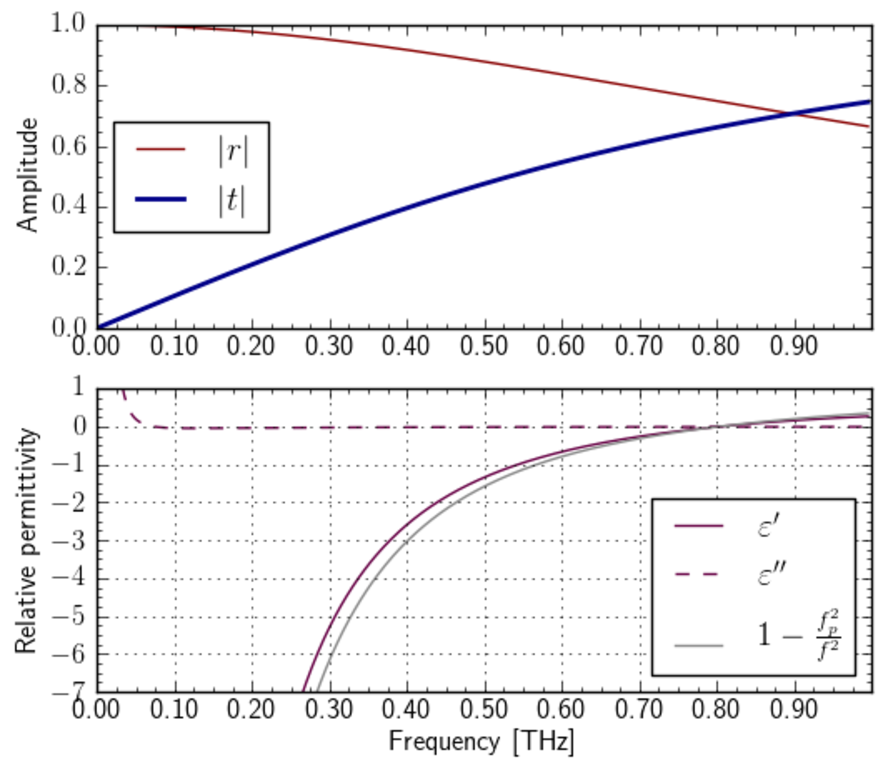
\includegraphics[width=11cm]{img/XCylWire_a100r4.pdf}
\end{figure}

Why does the transmission of a wire array differ from a metallic sheet? The key mechanism is that the current required to reflect the wave also causes the magnetic field to circulate around the wire. (This is similar to the difference between the dielectric rods $||\mathbf E$ and a homogeneous dielectric slab.) Each wire therefore behaves as a distributed inductor so it can no more entirely screen the incident electric field \cite{pendry1996extremely}. As a result, for any alternating field, always some nonzero amplitude is transmitted.

In terms of homogenized effective parameters, such a medium composed of infinite wires behaves as a "diluted metal" or plasma and its effective permittivity is finite at any nonzero frequency. The Drude model holds for low enough frequencies:
\begin{equation} \varepsilon_{\text{eff}} = 1 - \frac{f_{p}^{2}}{f^{2}} \label{eq_metaleps}\end{equation}
The permittivity is negative for frequencies below its plasma frequency $f_p$, at which $\varepsilon$ gets positive. The value of effective plasma frequency $f_p$ of the wire medium, depending on wire radius $r$ and grid spacing of $a>r$, is predicted by the analytic model\cite{maslovski2002wire} as:
\begin{equation} f_{p}^{2} = \frac{c^{2}}{2\pi \cdot a^{2} \cdot \ln\left(\frac{a^{2}}{4r \cdot (a-r)}\right)} \label{eq_fp_maslovski}\end{equation}
The more space is left around each wire and the smaller radius the wire has, the larger is its self-inductance and the lower lies the effective plasma frequency. 
Note that for a single cell, the transition from negative to positive permittivity is not accompanied by any obvious spectral feature on the reflection/transmission plot. 

We ran two series of wire array simulations (Fig. \ref{fg_omegap_a}) as a simple verification of both the FDTD algorithm and the mentioned analytic model. In the first series we kept the wire radius constant $r = 16\,\upmu$m  and changed the wire spacing $a$ (red points). For comparison, we plot in Fig. \ref{fg_omegap_a} the plasma frequency predicted by the Maslovski's analytic model\cite{maslovski2002wire} from Eq. (\ref{eq_fp_maslovski}) and by the older Pendry's model \cite{pendry1996extremely} (full and dotted lines, respectively). To test the possible error introduced by the FDTD algorithm, we ran the simulation with different resolution - results with fine $1$ $\upmu$m grid are denoted by full circles, results with coarse $4$ $\upmu$m grid with empty squares. Finally we also repeated this plot for thinner wire with $r = 8$ $\upmu$m.
\begin{figure}[ht] \caption{Comparison of numerical results and analytic model for plasma frequency $f_p$ of a wire medium. \textbf{a)} $f_p$ as a function of wire spacing, \textbf{b)} $f_p$ as a function of wire radius. } \label{fg_omegap_a} \centering 
\textbf{a)}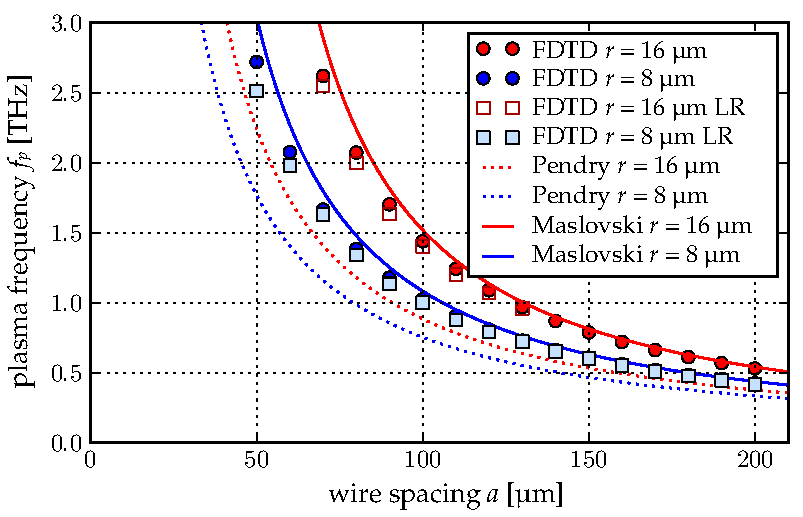
\includegraphics[width=8cm]{img/EWire_plasmaF_spacingscan.pdf}
\textbf{b)}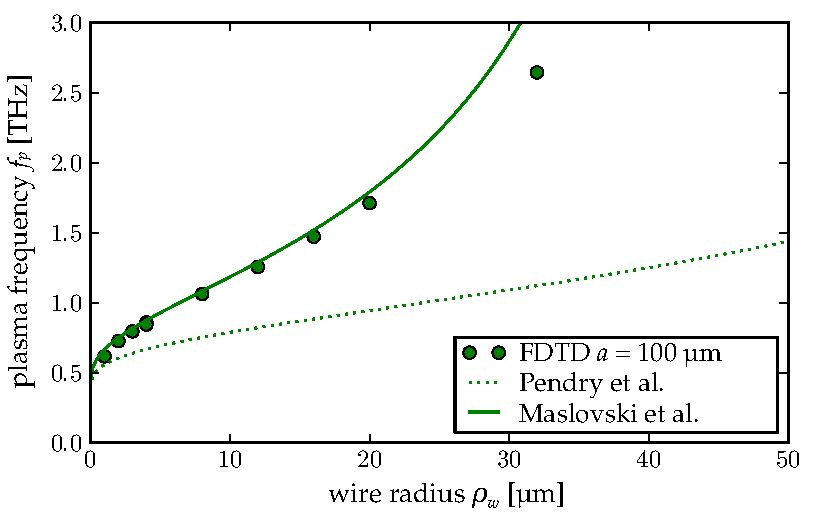
\includegraphics[width=8cm]{img/EWire_plasmaF_radiusscan.pdf}
\end{figure}

In the second series of simulations, we kept the spacing $a = 100\,\upmu$m and changed the wire radius $r$. The analytic model\cite{maslovski2002wire} and FDTD simulation give similar results (up to 5 \%) even for wire radii approaching roughly $a/4$. For thicker wires, the analytic model predicts higher plasma frequency than FDTD.  To conclude, the results of the model presented by Maslovski match the FDTD simulation with good accuracy for thin wires (where $r \lesssim a/5$). One possible application of the wire medium is in the construction of negative refractive index metamaterials, where a small negative real value of permittivity is desired.

% == History ==    artificial dielectrics, which were already designed in the 1940s for microwave frequencies -- J. Brown, “Artificial dielectrics,” Prog. Dielectr. 2, 193–225 (1960)


% \chapter{Metamaterials -- Critique and alternatives}
% TODO TODO At the end, the author would like to express his concern about the efficiency and practical impact of the metamaterial research in the last years. 
% 
% The name of this chapter is borrowed from the same-named book by Ben Munk \cite{Munk2004}. The book presents several objections against MM that seem to be ill-argumented and some of them seem to be also utterly wrong. However, as another point it also touches a really deep problem: the hypertrophic number of publications dissolves the concentration of pertinent ideas in almost a homeopatic way. Perhaps anybody interested in MM will soon notice there are many papers adding just a quantitative difference to what was already published, often without stating this important fact. This may give a superficial feeling of an exponential gathering of knowledge, but in fact it mostly contributes to the information noise. 
% 
% It is understandable that such a new (or at least newly recognized) scientific field exerts a great pressure to publish as much and as early as possible, which is exacerbated by the objective way of how the contemporary scientific work is evaluated. 
% That said, the situation is not as bad as it might seem and the author is also aware of several recent brilliant MM publications that give a deep insight into new physical phenomena.
%
% ** Subwl imaging: "if we can make deeply subwl inclusions, we can perhaps make slightly subwl near-field detectors"
% 
% Another question is the practical benefit of metamaterials for the humankind. 
% Compared to the publication boom and its optimistic aims, the metamaterials find their way to applications markedly slowly. The novel phenomena such as cloaking or sub-wavelength imaging are still confined to laboratory demonstrations, usually for structures not much bigger than the wavelength. The research of semiconductors in the first decades did not bring any notable applications, either, but even at that time it had to be clear that semiconductors present a wholly new field of basic material research. On the other hand, the recent progress in the field of metamaterials resembles the applied research: It is mostly a \textit{design} and \textit{optimisation} of already known structures towards some particular behaviour, rather than a search for new fundamental physics. 
% 
% Writing these lines, the author is not aware of any readily realized application where a metamaterial would present a significant advantage over classical structure. Will metamaterials ever find their application in any field of technology? And if not, will at least some of the developed theory or methods be useful in the future?
% 
% To conclude this pessimistic, but well meant section, the author


%%26. Y. Fu, L. Thyl ́n and H. Agren, “A Lossless Negative Dielectric Constant from Quantum e Dot Exciton Polaritons,” Nano Lett. 8, 1551 (2008).
%%27. A. Bratkovsky, E. Ponizovskaya, S. Y Wang, P. Holmstr ̈m, L. Thyl ́n, Y. Fu, and o e H.  ̊gren, “A Metal-wire/Quantum-dot Composite Metamaterial with Negative ǫ and A Compensated Optical Loss,” Appl. Phys. Lett. 93, 193106 (2008).
%%28. Y. Zeng, Q. Wu and D. H. Werner, “Electrostatic Theory for Designing Lossless Negative Permittivity Metamaterials,” Opt. Lett. 35, 1431 (2010).


\chapter{Conclusion}
We presented experimental and theoretical studies of simple periodic structures -- the periodic arrays of dielectric slabs, two orientations of rods, dielectric spheres, metallic wire mesh, as well as a composite of spheres and a mesh. An attempt was made to make an analysis of the modes that are responsible for the photonic bands, illustrating different electromagnetic phenomena and their dependence on a structure parameter. An analytic model for wire medium was proven to match our numerical results.
The prospects for the future work are to broaden this catalogue to other structures in order to enable comparison and deeper physical interpretation of their behaviour. 


A versatile numerical environment for simulations was prepared and tested in the last two years. All computation scripts, containing over 2000 lines of Python code, are open-source and they use freely-redistributable libraries only, which may be useful for the broader scientific community in the future. 
The automated effective parameters retrieval from FDTD is especially suitable for parametric scans. It proves instrumental in optimisation of the structure performance, matching experimental data, as well as studying the tunability.

Broad range of physical phenomena may be included in the simulations. A library of realistic permittivity models is being built that allows to match TDTS experiments with a good accuracy. It is also possible to combine dispersive dielectrics with metals and doped semiconductors. 
 The FDTD method is applicable also to non-periodic, lossy and time-changing structures, while PWEM enables e. g. studies of the magnetooptic phenomena.
All referred numerical methods, FDTD, PWEM and TMM, were tested also to give compatible and plausible results under oblique incidence and both TE/TM polarisations. 

Some of the numerical simulations are also planned to be tested on the experimental basis. One of the proposed structures is an array of spheres embedded in a double metallic mesh. This structure is predicted to exhibit negative refraction in a narrow transmission band, and moreover, if the spheres are made of strontium titanate, which is a high-permittivity ferroelectric, the frequency of this band can be tuned by temperature or electric voltage between the metallisation. Other experimental work will focus on extraordinary transmission in metallic fishnets and tunable planar metamaterials. In all cases the experiments will be supported by thorough numerical simulations and possibly also by analytical models.

\chapter{ebars 2014}
In the studies of electromagnetism of photonic structures with a sub-wavelength
periodicity, two main concepts have been employed: that of electromagnetic metamaterials
(MM) and that of photonic crystals (PhC). In both classes of structures, their properties
are due to resonant behavior of the structure at particular frequencies of the
electromagnetic field.
\begin{enumerate}
\item {
In MMs, the energy of the resonant field is localized in a small fraction of the unit
cell volume, which is usually in/near a resonator made of metal or high-permittivity
dielectric ($\varepsilon_r \gg 10$) \cite{vendik2012tunable}. 
The coupling of the resonant field between
neighboring cells is negligible, so the MMs have a small enough spatial dispersion and
their behavior can be described using frequency-dependent effective parameters: the index
of refraction $\Neff$, wave impedance $\Zeff$, permittivity $\eeff=\Neff/\Zeff$ and
permeability $\meff = \Neff\cdot \Zeff$.
}
\item{
By contrast, PhCs are typically made of low-permittivity dielectrics ($\varepsilon_r
\lesssim 12$) which often fill a larger part of volume than what is usual in MMs. The
resonances are strongly influenced by the presence of neighboring unit cells as they rely
on constructive and destructive interferences between scattered (partially reflected)
waves. As a result, the iso-frequency contours of two-dimensional (or three-dimensional)
PhCs often deviate from elliptical (or ellipsoidal) shapes.

In such a general case, the angle of refraction at a PhC interface cannot be computed
using the Snell formula, and it is impossible to use the notion of the
refractive index $N$ in its general sense. Nevertheless, it is possible to find directions of
propagation (namely those parallel to the symmetry axes) where the iso-frequency contours
can be locally approximated by ellipsoidal shape. Close to such directions the
Snell law holds approximately and one may introduce effective indices of
refraction of the PhC for these particular directions \cite{yannopapas2005negative}.
}
\end{enumerate}

It appears, however, that some kinds of photonic structures represent intermediate cases
between PhCs and MMs; this fact did not receive much attention so far. One of the
simplest examples is a square array of cylindrical dielectric rods, oriented parallel to
the electric field of the incident wave; this geometry was treated as a photonic
crystal\cite{plihal1991two} and later as a metamaterial\cite{zhao2009mie,Vynck2009, felbacq2009}. The
effective response of the rod array depends on two parameters only---the ratio of the
unit-cell size $a$ to the rod radius $\rho$, and the dielectric permittivity of the rods
$\varepsilon_r$, whose imaginary part is assumed to be negligible in this paper. Our aim is to
find out which interesting qualitative changes in behavior can be found when these parameters
are continuously changed.

%% TODO reference!
From the practical point of view, the requirement of a high permittivity $\varepsilon_r
\gg 10$ not only restricts the choice of materials but also determines the frequency
range where such values can be attained. 
\cite{zhao2008tunable,zhao2008experimental}
As a rule, the permittivity in dielectrics
decreases in average with frequency except for narrow intervals around resonances, which
are always accompanied by an increased absorption. In this paper, we focus on the microwave and terahertz
range where materials with a high $\varepsilon_r$ exist and the structures can be relatively easily fabricated
\cite{nemec2012resonant,nemec2009tunable}. We restrict our computations to the normal
incidence which implies the propagation along the mirror plane inside the photonic
structure; in this case the notion of the refractive index can be used even when the
structure is in the PhC regime.

In the paper we discuss numerical results obtained during a systematic variation of the
structure parameters. Namely, we show that their relatively minor variations can lead to
a qualitatively changing optical response. We also discuss the somewhat surprising experimental 
results which were previously published  \cite{peng2007}
and summarize the implications for building optical MMs from dielectric rods.

\section{Calculation of effective parameters}

Our structure is defined by a square unit cell with the linear dimension $a$ periodically
distributed in the $yz$ plane; the dielectric rod parallel to $x$-axis with radius $\rho$
and permittivity $\varepsilon_r$ is positioned in its center. We employed the
finite-difference time-domain (FDTD) simulation package MEEP \cite{oskooi2010meep} to
obtain the scattering coefficients (complex reflectance $r$ and transmittance $t$) of a
structure with variable number of unit cells along the wave vector direction $k\parallel
z$. The incident wave is polarized $E\parallel x$, periodic boundary conditions were
applied in the $y$-direction. We found that for this geometry the retrieved effective
parameters depend only negligibly on the number of unit cells in the $z$-direction.
Therefore we performed the majority of simulations for a single unit cell only which can
be considered as a thin film with effective properties remaining valid also for the
corresponding bulk structure. The effective parameters were retrieved from complex
transmittance and reflectance spectra \cite{smith2002determination}; in addition, we
developed an algorithm ensuring that the solution is unambiguous, as described in the Appendix.
The retrieved value of the complex effective index of refraction $\Neff(f)$ defines the
magnitude of the wave vector
\begin{equation}\label{eq_wave_vector}
k(f) = 2\pi f \Neff(f) /c\,.
\end{equation}
Note that the retrieval procedure described in the Appendix implies that the wave vector
introduced by Eq (\ref{eq_wave_vector}) is defined in an unfolded reciprocal space. 

A Bragg resonance occurs when an integer number of half-wavelengths fit into one unit cell, i. e.  when
\begin{equation}\label{eq_BZ}
k(f) = \frac{q \pi}{a}\,,
\end{equation}
where $q$ is a non-zero integer. In such a situation the wave vector is located at a
Brillouin zone boundary. The purely real values of $k$ then describe photonic band edges.
In a band edge state, a standing wave appears in the structure and it is characterized by
exactly $q$ nodal planes sectioning each unit cell in the transverse direction to $q+1$
disconnected parts. The band edges delimit a photonic {\itshape Bragg band gap} where
only evanescent waves described by $\Neff''>0$ can exist.
We can write an equation analogous to (\ref{eq_BZ}) for the real part of the refractive
index:
\begin{equation}\label{eq_BZN}
\Neff'(f) = \frac{q c}{2 a f}\,;
\end{equation}
its hyperbolic behavior versus frequency reflects the pinning of the wave vector to the
Brillouin zone boundary inside the Bragg band gap.

Another case of interest where evanescent waves are obtained is that of $\Neff' = 0$
(center of the first Brillouin zone, $q=0$) and $\Neff''>0$. Here the waves exponentially
decay in the medium without any phase change. However, this behavior has a different
origin: it is connected to a plasma-like response of the material ($\varepsilon<0$ or
$\mu<0$) and in this paper we use the term \textit{plasma band gap} to refer to it.

The Kramers-Kronig relations require that for any structure studied, $\Neff'(f)$ [or,
equivalently, $k(f)$] attains and finally crosses the Brillouin-zone boundaries when the
frequency is sufficiently increased. While usually the convention is used that the
corresponding curves are folded back into the first Brillouin zone, in this paper we plot
$\Neff'(f)$ in the original (unfolded) Brillouin zones resulting from the retrieval
algorithm. This can be clearly observed on the dispersion of the refractive index in
Fig.\ \ref{fg_spec}. In this way we retain the information about the number of the nodal
planes intersecting the unit cell, which is important for our discussion.

\section{Results}
\begin{figure}[h!]
%\centering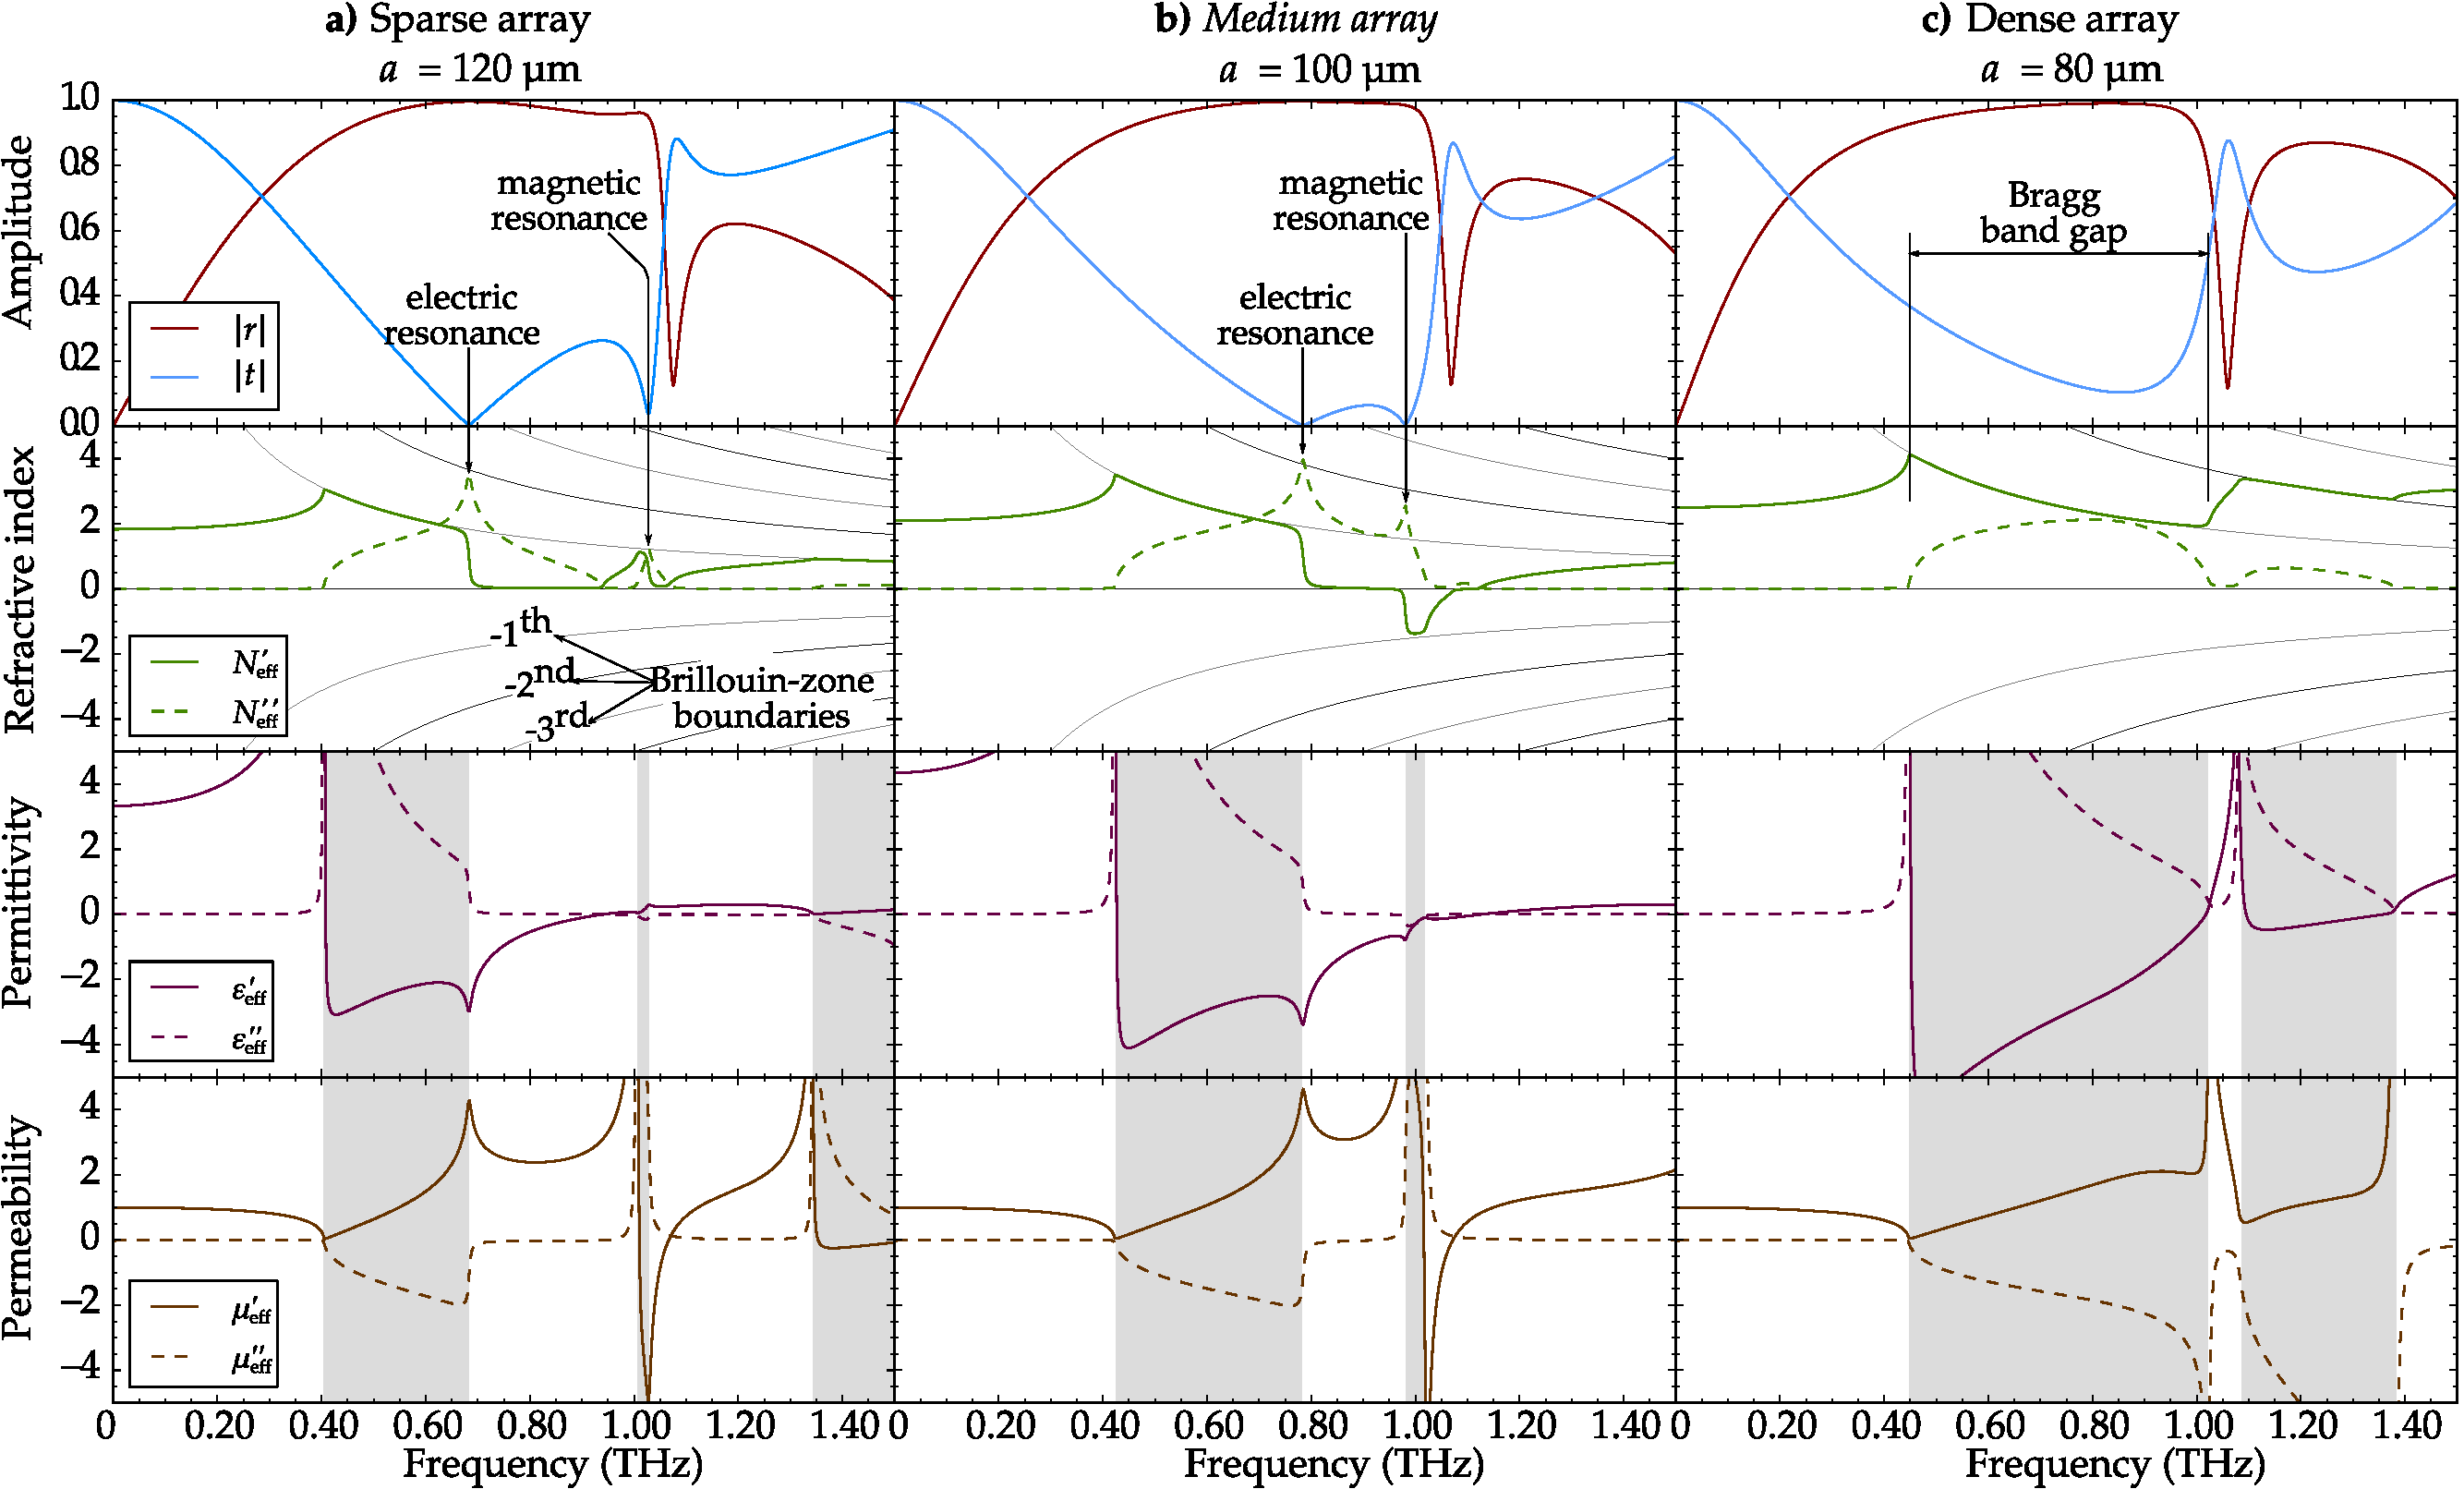
\includegraphics[width=16cm]{img/ERods_eps100_triple_a150a100a080_FDTD.pdf}
\centering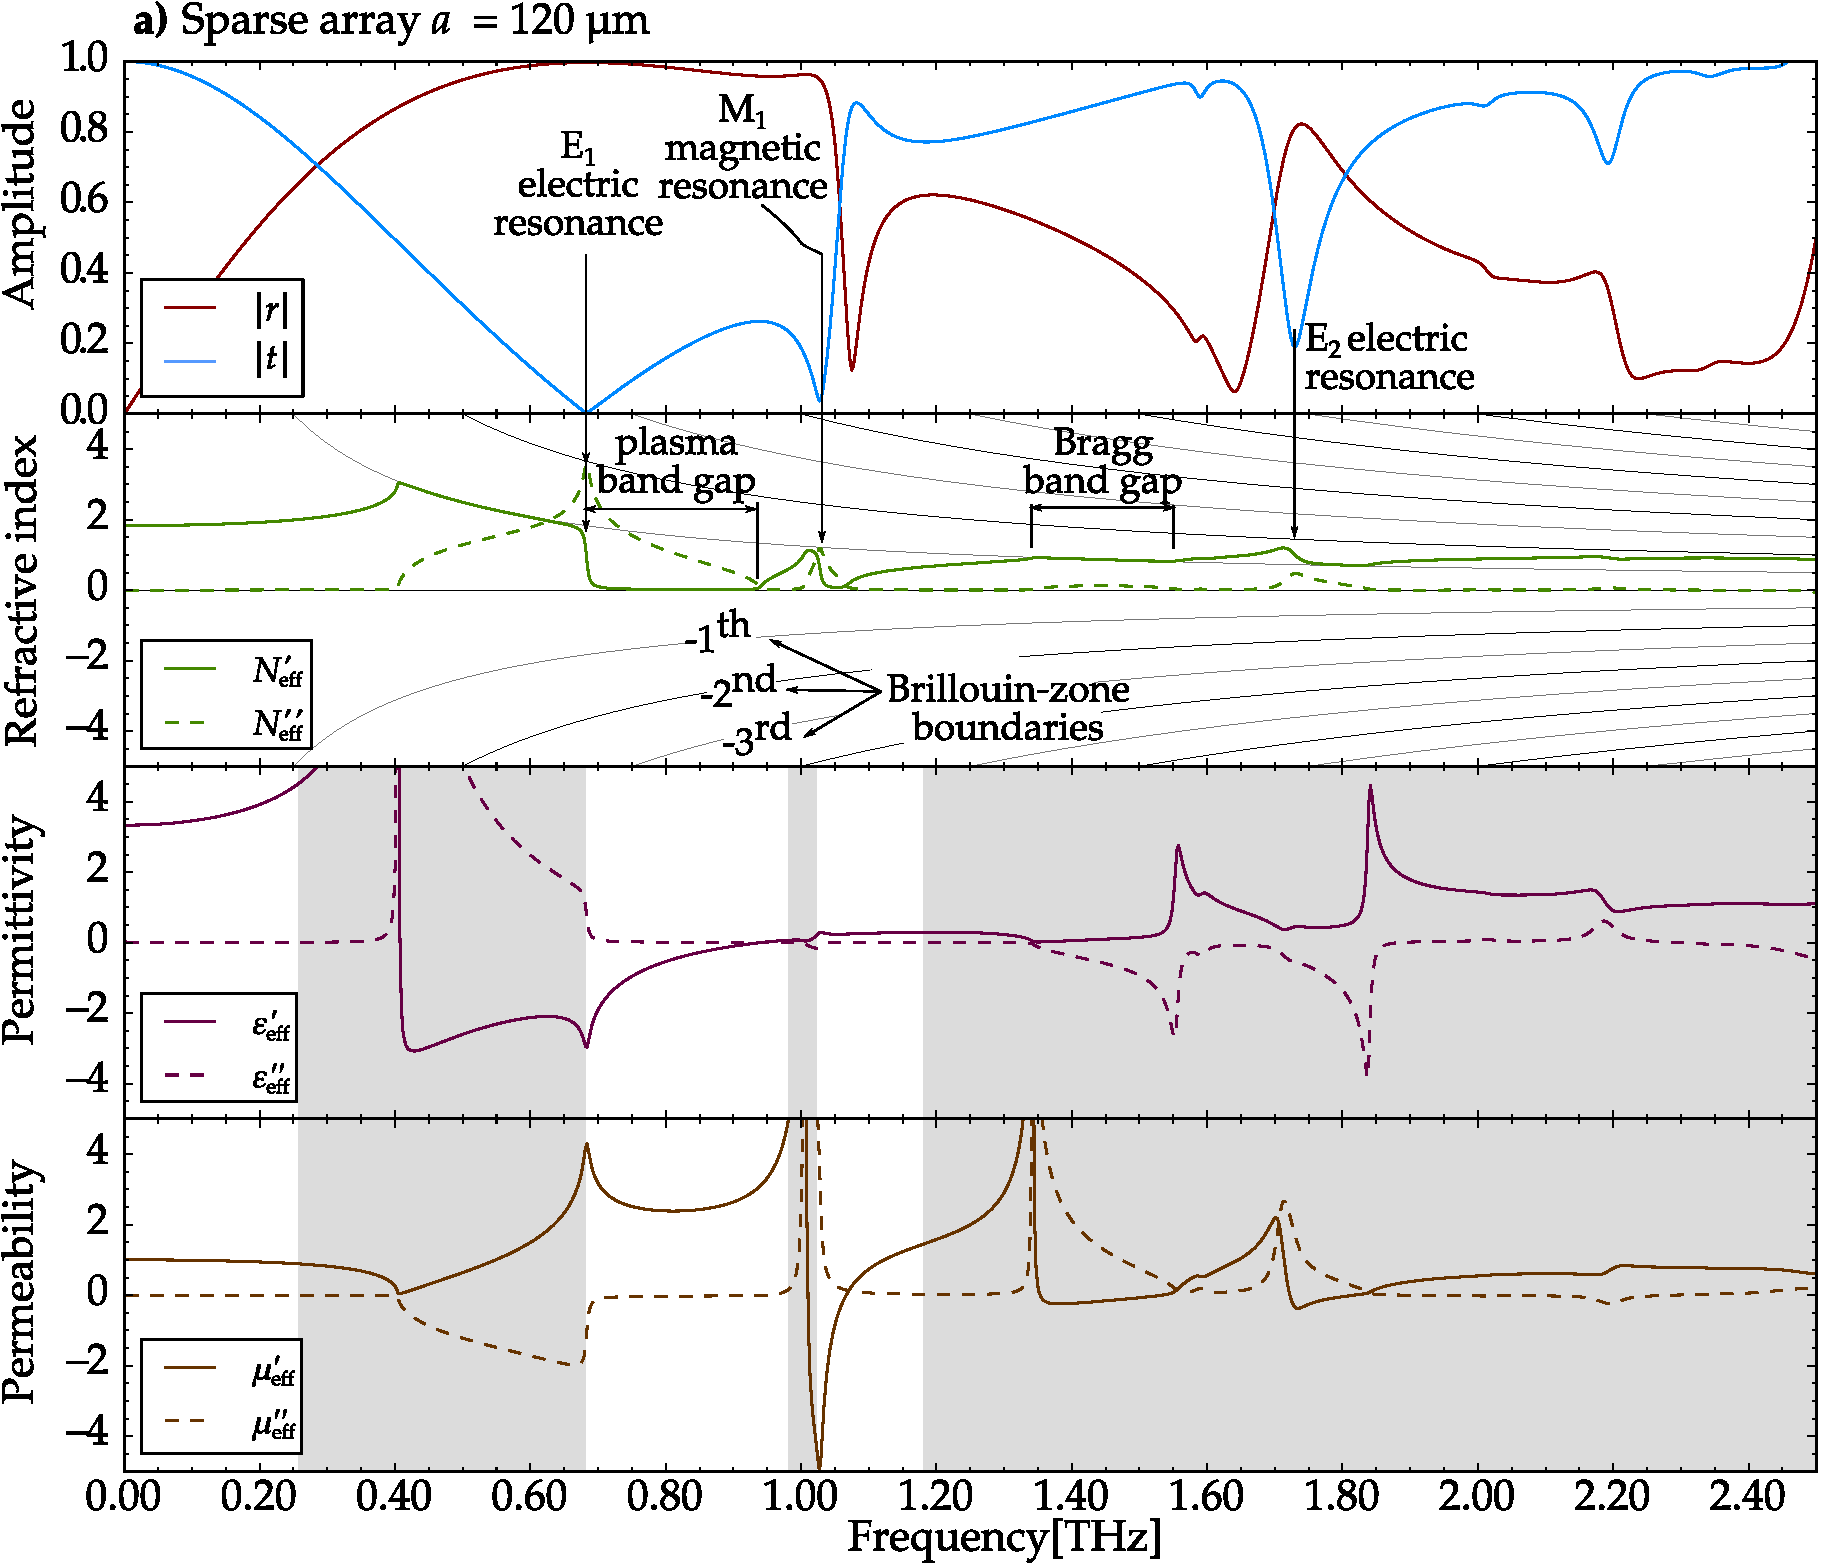
\includegraphics[width=11cm]{img/ERods_eps100_single_a120_FDTD.pdf}
\centering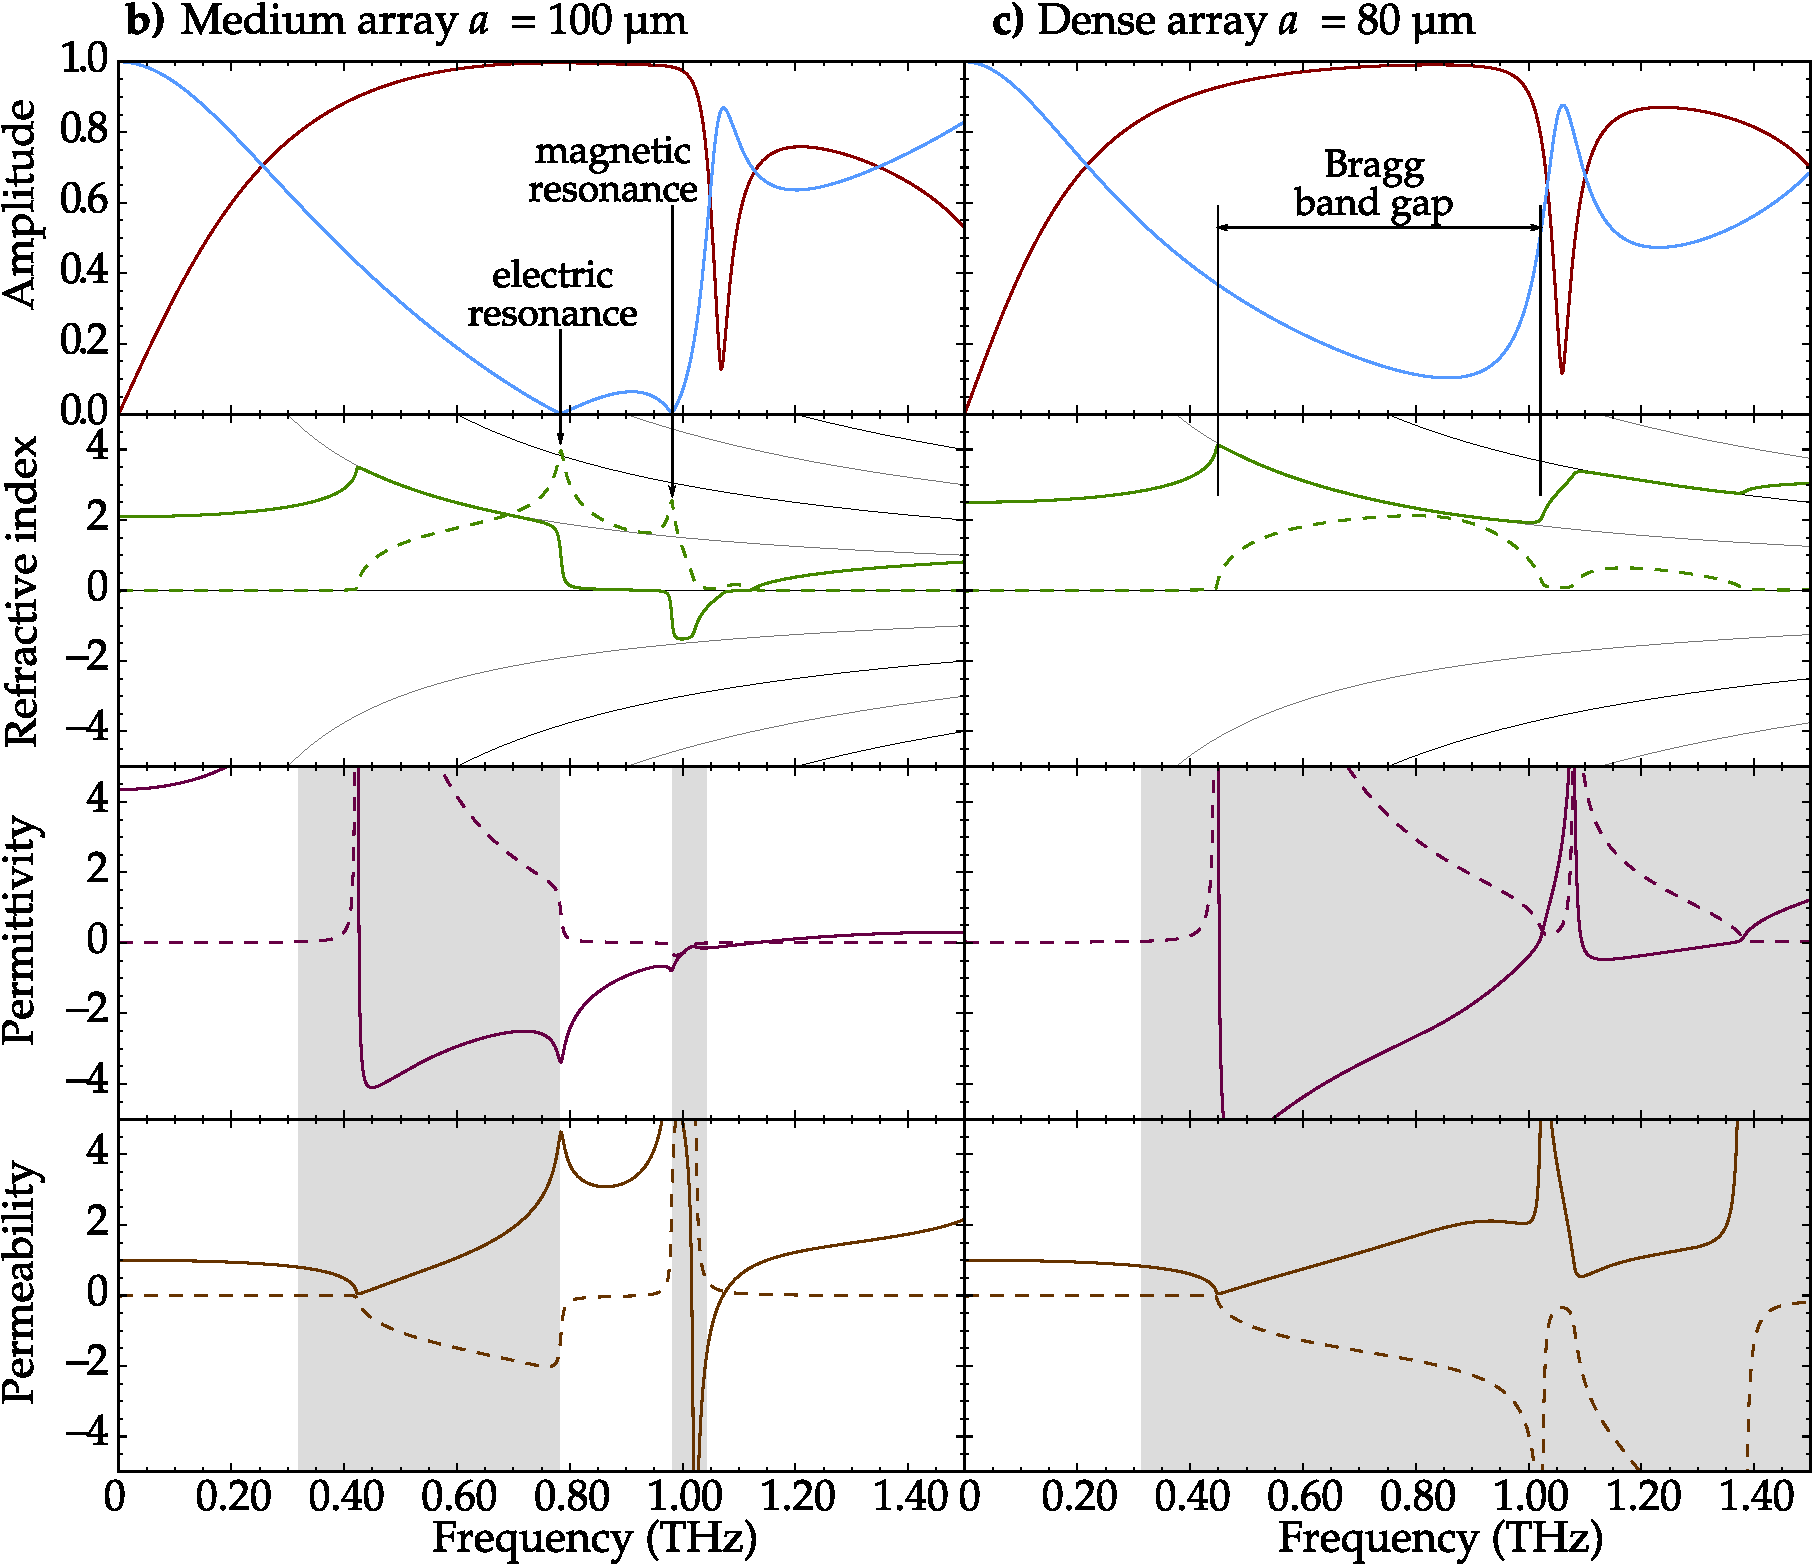
\includegraphics[width=11cm]{img/ERods_eps100_double_a100a080_FDTD.pdf}
\caption{Results of the FDTD simulations for a single layer of dielectric rods with $\varepsilon_{\rm r}= 100$,
$\rho=10$\,$\upmu$m. The spectra of reflection $|r|$ and transmission $|t|$ amplitudes share
their frequency axes with the retrieved complex effective index of refraction $\Neff$,
permittivity $\eeff$ and permeability $\meff$, whose imaginary parts are denoted by
dashed lines. The frequency ranges where $\eeff$ and $\meff$ have no physical
interpretation (Bragg band gaps or higher order photonic bands) are gray shaded.  } \label{fg_spec}
\end{figure}
% NOTE: dispersive permittivity was 100+0.8 (at 1 THz)

%\comm{only $\Neff$, $\eeff$, $\meff$; best layout would be: (a) 120 $\upmu$m up to 2.5 THz (for
%comparison with Fig. 4) and magnified over the page width on first panel; (b,c) on second
%panel below with the current scale up to 1.5 THz but magnified nearly over the page
%width; what imaginary part was used for calculations in reality?} 

In the following we first describe in detail three characteristic cases: we compare the
effective parameters computed for three slightly different unit-cell sizes while the rod
radius and the dielectric permittivity are fixed. The comparison of these cases reveals quite
remarkable changes in the optical behavior of the structure. We then complement this
comparison by a continuous scan of the unit-cell sizes in order to obtain an overview of
all possible types of the response for the rod-based geometry.

In Fig.~\ref{fg_spec}, we show the calculated reflectance and transmittance amplitude
spectra, as well as the effective parameters of three representative structures which
have the same rod radii $\rho = 10$~$\upmu$m, but they differ by the unit-cell size $a =$ 120, 100 and 80 $\upmu$m. These
values of $a$ were selected to illustrate three qualitatively different regimes of
behavior.
The dielectric was defined by a simple lossy model with one high-frequency oscillator, its  permittivity was $\varepsilon_r = 100.1 + 0.5\mathrm{i}$ at 500 GHz.


\paragraph{Sparse array}
In Fig.~\ref{fg_spec}(a), where the unit-cell size $a=120$~$\upmu$m, we can see two well
separated Mie resonances: the electric one at 680 GHz and the magnetic one at 1030 GHz.
The field distribution of the corresponding modes is sketched in
Fig.~\ref{fg_sketchfield}. The resonance frequencies can be easily identified by an
abrupt drop in the real part of the effective index of refraction $\Neff'$, accompanied
by a sharp peak in its imaginary part $\Neff''$. The Mie resonances in periodic media
without losses must always neighbor a Bragg band gap. For instance, in
Fig.~\ref{fg_spec}(a) at frequencies below the first Bragg gap, the electric dipoles
within each rod are directed along the electric field in the rest of the unit
cell. The rods thus positively contribute to the refractive index $\Neff'$ which
progressively grows until it reaches the first Brillouin zone boundary. At this point the
Bragg condition for a photonic band-gap is fulfilled and each unit cell is intersected by
one nodal plane. This is reflected by the dispersion of $\Neff'(f)$ which follows the
first Brillouin-zone boundary in the first Bragg band gap between 400 and 680\,GHz [equivalent to $q=1$ in Eq. (\ref{eq_BZN})]:
$$	\Neff'(f) = \frac{c}{2af}\,. $$
At 680\,GHz the electric Mie resonance occurs which dramatically changes the near-field
photonic properties of the structure. The observed drop in $\Neff'(f)$ and the slope change
in $\Neff''(f)$ mark the plasma-like character of the adjacent part of the band gap which
extends up to the plasma frequency of the Mie resonance (940\,GHz). In this frequency
range the electric dipoles in the rods change their direction and induce an electric field
opposite to the incident one.

For this sparse array of dielectric rods the first magnetic Mie resonance lies at
1030\,GHz, above the plasma frequency of the electric mode. 
The second Bragg band-gap opens at 1010 GHz and, due to the Mie resonance, it is transformed to a plasma band gap at 1030 GHz. The next allowed photonic band starts above magnetic plasma frequencies at 1070 GHz.
Therefore we observe a completely analogous behavior near the magnetic resonance. 

For completeness we note that at 1350 GHz, a third Bragg band gap
starts which, unlike the lower-frequency ones, does not contain any Mie resonances 
[see Fig.\ \ref{fg_spec}(a)].

\begin{figure}[h]
\centering 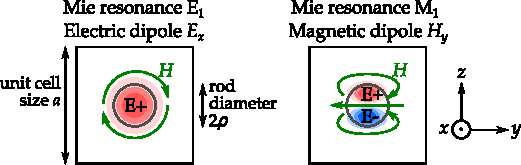
\includegraphics[width=9cm]{img/ERods_1st_and_2nd_Mie_resonance.pdf}
\caption{Sketch of the unit-cell
cross-sections with the resonant modes excited by a plane wave with $\mathbf{E}||x,
\mathbf{H}||y$ and $\mathbf{k}||z$. The first Mie resonance has an electric dipole moment
only, while the second one has a magnetic dipole moment instead. The red-white-blue color
corresponds to the $E_x$ component of the electric field, while the magnetic field is
represented by the arrows. }\label{fg_sketchfield}
\end{figure}

The resonances in the effective permittivity $\eeff=\Neff/\Zeff$ and permeability $\meff
= \Neff\cdot \Zeff$ of a periodic array obviously exhibit shapes very different from the
well-known resonance curves of a damped oscillator\cite{koschny2003resonant}. In the two
separate plasma band gaps we obtain either $\eeff < 0$ or $\meff<0$, i.e. the usual
behavior observed in the reststrahlen bands of resonances. However, in the Bragg band
gaps occurring just below these spectral ranges the behavior of $\eeff$ and $\meff$ does
not have any useful physical interpretation and it can be understood as a purely formal
frequency dependence: we shaded these ranges with light gray in Fig.~\ref{fg_spec}.

\paragraph{Medium array}
When the unit cell size is reduced to $a=100$~$\upmu$m, as depicted in
Fig.~\ref{fg_spec}(b), the Mie resonances shift slightly. Interestingly, the electric
resonance frequency increases from 680 to 780 GHz, that of the
magnetic resonance decreases from 1030 to 980 GHz. This can be explained by the
inter-cell coupling: the circulating magnetic field of the first resonance is compressed
when the rods get closer, whereas the magnetic dipoles of the second resonance can couple
more easily to each other in the same situation (see Fig.~\ref{fg_sketchfield}).

The converging of the resonance frequencies is linked to the most important
qualitative change in the spectra: the fact that the magnetic resonance occurs at a
frequency where $\eeff'<0$. The first band gap (lowest continuous frequency region where
$\Neff''>0$) is thus composed of three adjacent regimes: the first Bragg band gap
(425--780 GHz), a plasma band gap (780--980 GHz) and the second Bragg band gap (980--1020
GHz). Every Mie resonance introduces a drop in $\Neff'$, so the following photonic band
(1020--1070 GHz) features a negative index of refraction ($\Neff'<0; \Neff''\approx 0$),
i.e. the phase and group velocities are opposite to each other. We conjecture that the presence of two
Mie resonances in the \textit{first} combined band gap is a necessary and sufficient condition for
$\Neff'<0$ to occur.
% TODO: \cite{shi2007effects} this cite should be elsewhere

Note that the transmittance amplitude reaches quite small values in between the Mie
resonances when they are sufficiently close to each other [Fig. \ref{fg_spec}(b)]. This range forms a
well-defined band with a reflectance-to-transmittance contrast much better than that
observed in a planar Fabry-P\'erot resonator. One layer of dielectric rods with proper
parameters can therefore be applied as a thin, yet very high-contrast filter.

\paragraph{Dense array}
Perhaps an even more surprising change occurs when the rod spacing is further reduced. The Mie resonances get even closer in the
spectrum and eventually they vanish for $a=80$~$\upmu$m [see Fig.~\ref{fg_spec}(c)]. The band gap remains at nearly the same spectral
position as in panel (b) of this figure, but, unlike for the medium array, the value of $\Neff'$ does not drop within
the Bragg band gap. In contrast, it is shifted up to the second Brillouin zone boundary
where it meets the second Bragg band gap as clearly seen in panel (c), indicating that
each unit cell is intersected by two nodal planes in this state.

The reason of this behavior is related to the change of the nodal plane topology caused
by the inter-cell coupling. When the rods are far from each other ($a\gtrsim
100$~$\upmu$m), the individual Mie resonances create closed regions delimited by a nodal
surface where the fields are opposite to the rest of the unit cell. Upon reducing the
unit-cell size ($a\lesssim 80$~$\upmu$m), the regions of opposite fields start to overlap
with those from the neighboring cells and the corresponding nodal surfaces interconnect
and open. This pair of open nodal surfaces dividing the unit cell manifests itself by a
qualitative change of the $\Neff'$ spectrum towards a shape typical for one-dimensional
photonic crystals.

% [from ~/p/MEEP_2013/130711_EWires/47bd_Diel100_SpacingScan_EquiLossLong/effparam]
%\comm{Please remove upper labels from the figure, please make the font slightly larger,
%units in standard parentheses; why don't we see a negative index value at 100 $\mu$m and
%slightly below? Can the negative values be colored e.g. in red?}
\begin{figure}[h]\centering
    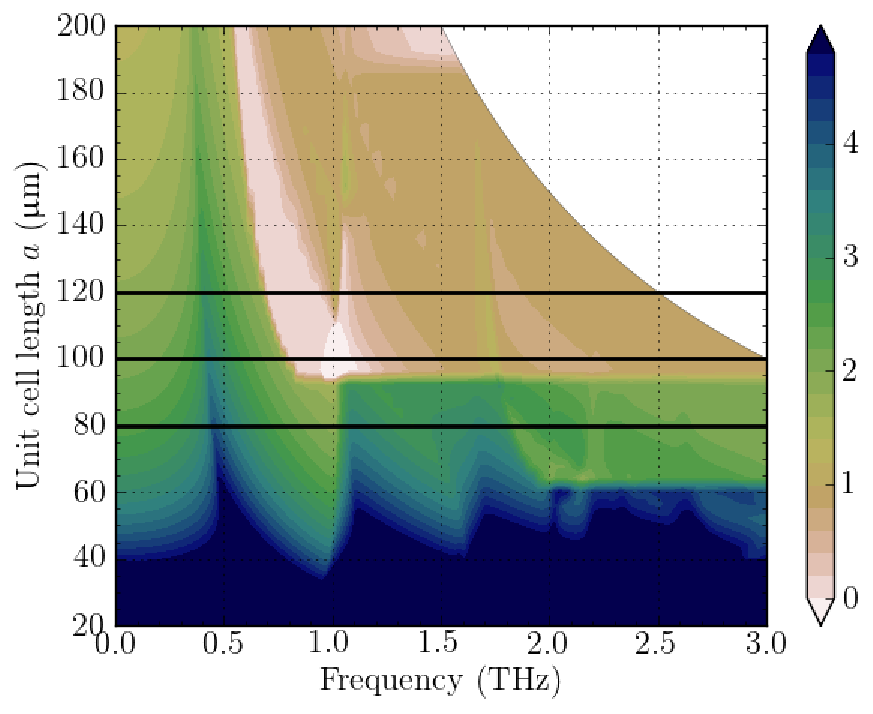
\includegraphics[width=8.5cm]{img/ERods_eps100_spacingscan_Nim.pdf}
    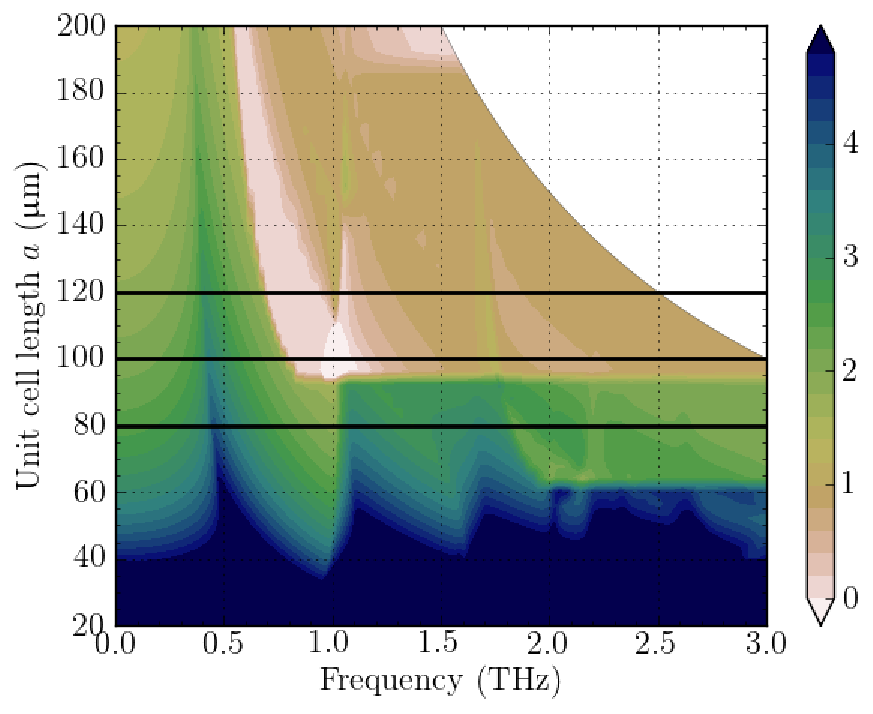
\includegraphics[width=8.5cm]{img/ERods_eps100_spacingscan_Nre.pdf}
\caption{Real ($\Neff'$, left panel) and imaginary ($\Neff''$, right panel) parts of
refractive indices for a dielectric rod array with permittivity $\varepsilon_r =100$,
radius $\rho = 10$ $\upmu$m and a variable unit cell size $20\:\upmu$m $<a<200\:\upmu$m. 
The three solid horizontal lines correspond to the values used in Fig.~\ref{fg_spec}.}
\label{fg_spacingscan100}. 

\end{figure}

\paragraph{Continuous scan of the unit-cell size}
The behavior described above is confirmed by the plots of the complex index of refraction
$\Neff',\: \Neff''$ for a continuously varying unit cell size $a$ from 20 to 200~$\upmu$m
(Fig.~\ref{fg_spacingscan100}). Here, again, the constant values of the dielectric
permittivity $\varepsilon_r=100$ and the rod radius $\rho=10$ \um are used. In the
upper-right corner of both plots, for $a>c/f$, an empty area is left where the
diffraction prevents the determination of effective parameters. 

For an easier interpretation of the results, we draw the most prominent features
schematically in Fig.~\ref{fg_drawn100}. Some of them are common in ordinary
one-dimensional photonic crystals, namely, the photonic (Bragg) band gaps which are
painted in color in Fig.~\ref{fg_drawn100}.

%\comm{Please add zoom, made on the interesting region
%	between segments 1 and 2 (say from 0.6 THz up to 1.4 THz and from a = 50 um
%	to 130 um); it can be delimited e.g. by a thin dotted line rectangle in the main
%	figure;  full color: only Bragg band gaps, hatched brown color:
%	plasma band gap (there will be only one); put units in standard parentheses; remove mid-gap
%	frequency line; type: onset of "the" diffraction. We must consider to show a similar figure for
%	a small permittivity of rods (e.g. 50 or 12)}
\begin{figure}[h]
  \centering
    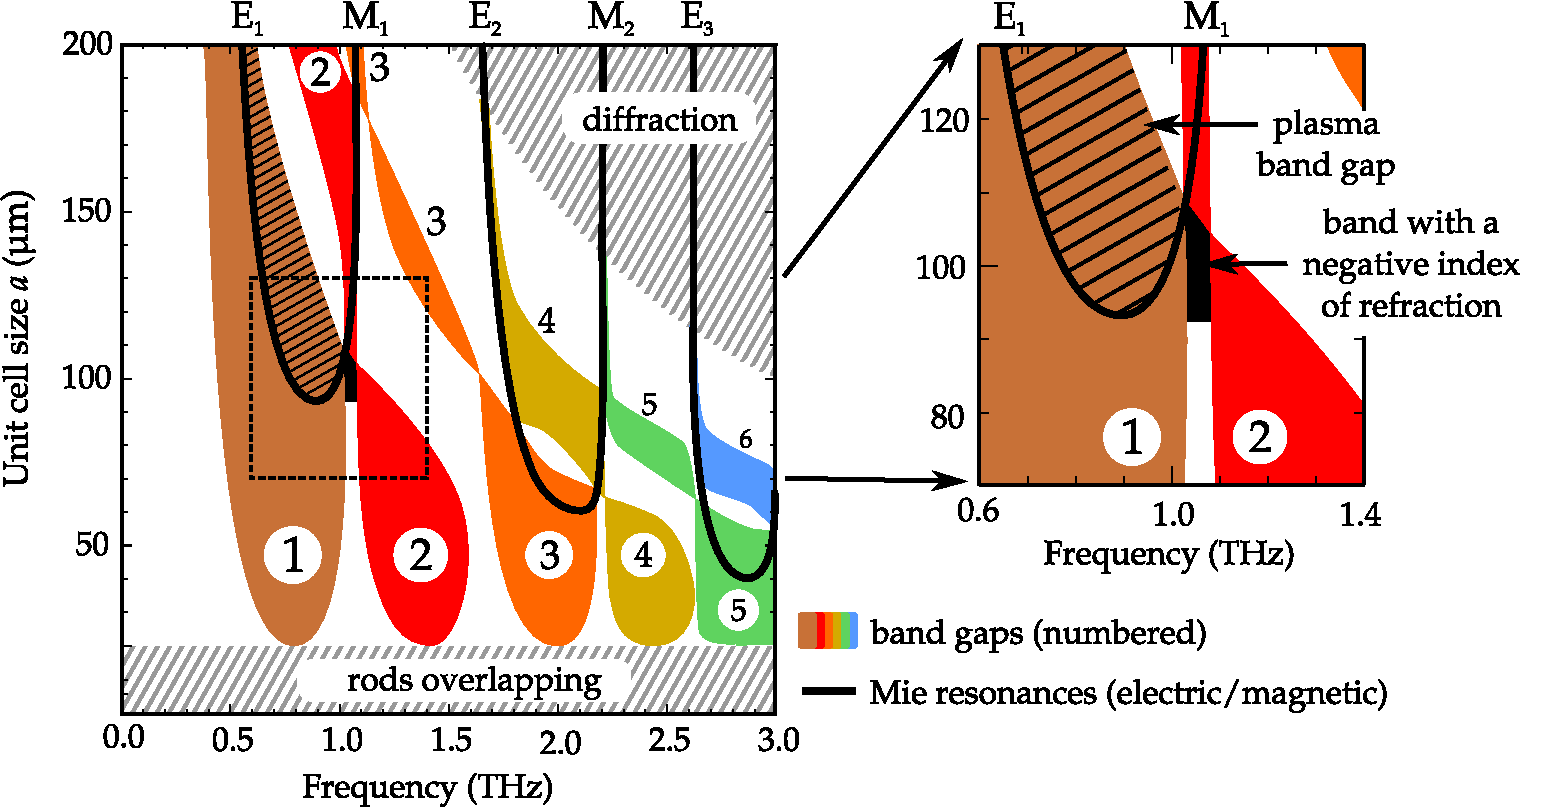
\includegraphics[width=14cm]{img/ERods_eps100_spacingscan_drawn_bands.pdf}
    \caption{Scheme of band gaps and Mie resonances under the same conditions as
    in Fig.~\ref{fg_spacingscan100}.}
\label{fg_drawn100}
\end{figure}

The Mie resonances are caused by the field confinement near the high permittivity
elements. They always manifest themselves as sharp peaks in the imaginary part of the
index of refraction ($\Neff''$), and in Fig.~\ref{fg_drawn100} they are denoted by thick
solid curves. Their electric- or magnetic-dipole character is identified by the letters
"E" or "M" above the plot, respectively.

As it can be seen in both Figs.~\ref{fg_spacingscan100} and \ref{fg_drawn100}, the pairs
of electric and magnetic Mie resonances form U-shaped curves, at the bottom of which the
resonances come closer in frequency to each other and eventually they disappear when the
unit-cell size $a$ is further reduced. The resonances influence the whole spectra of the
refractive index $\Neff'$, so the position of this U-curve delimits the range of $a$ for
which a photonic band with $\Neff' < 0$ and $\Neff'' \approx 0$ can be found. This
negative-index band is painted in black in Fig.~\ref{fg_drawn100}.

% from /home/filip/p/MEEP_2013/130711_EWires/47le_Diel30_SpacingScan_MediLossHR/effparam
\begin{figure}[h]
  \centering
    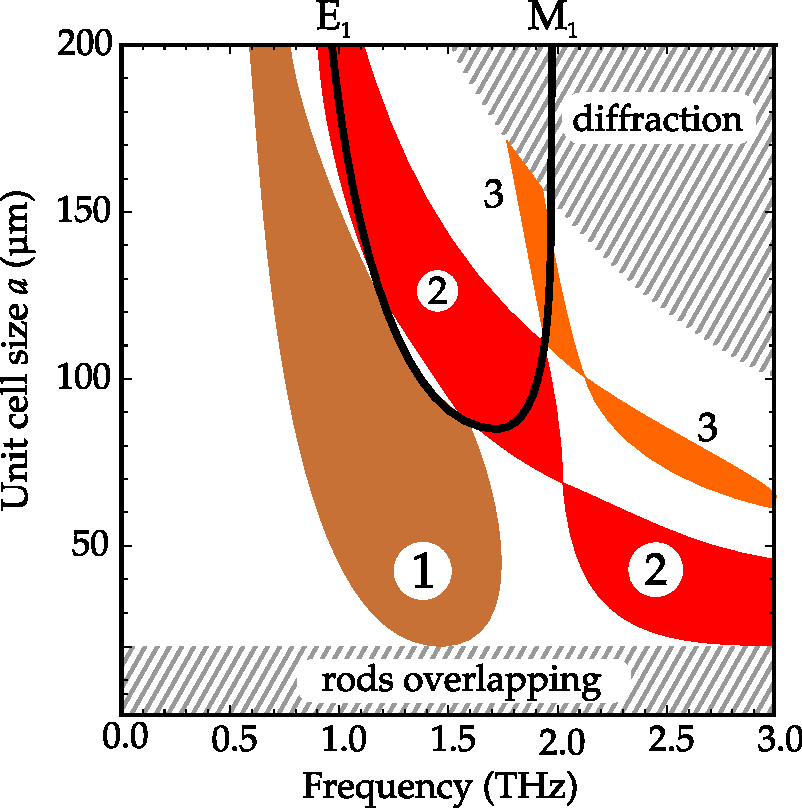
\includegraphics[width=7.2cm]{img/ERods_eps030_spacingscan_drawn_bands.pdf}
    \caption{Scheme of band gaps and Mie resonances for dielectric permittivity $\varepsilon_r = 30$. The Mie resonances shift to higher frequencies relative to the band gaps and no $\Neff'<0$ region is formed for any unit cell size (cf. Fig. \ref{fg_drawn100})}
\label{fg_drawn030}
\end{figure}

Note that the frequencies of the Mie resonances deviate from their free-space value when
the rod distance is reduced. In fact, these resonances help to form the photonic band
gaps (both Bragg and plasma band gaps) due to their dispersion. As a consequence these
resonances must be always located inside a frequency range with $\Neff''>0$.

\section{Discussion}
Having analyzed the case of high dielectric ($\varepsilon_r=100$) permittivity rods, we
will draw below implications for building a negative-index MM from available dielectrics.
Another series of simulations implies that reducing the dielectric permittivity has the main effect
to shift all the Mie resonances to higher frequencies (also compared to the photonic
bands). As a result, the band with $\Neff'<0$ gets gradually narrower and, for the rod
permittivity below about 50, we do not find any cell size $a$ that would imply the first
and second Mie resonances in the first photonic band as illustrated for $\varepsilon_r = 30$ in Fig. \ref{fg_drawn030}. This means that the value of
$\varepsilon_{r} \approx 50$ is the minimum for obtaining a negative index of refraction
in any square array of cylindrical rods. Note that one would come to a very similar value
of minimum permittivity for the case of a square array of bars with a slightly different
shape, e.g. a square cross-section. 

A sufficiently high permittivity can be found in the microwave and terahertz ranges, 
in a variety of materials, for example in titanium dioxide with $\varepsilon_r \approx 92$ \cite{nemec2009tunable} 
or in various ferroelectrics like strontium titanate \cite{skoromets2011tuning}. However, practical applications of
the high-permittivity dielectrics in the THz range can be restricted by high dielectric
losses due to low-frequency phonon absorption tails. To our knowledge, there is no
material providing such a high permittivity in the near-infrared or optical ranges. This
eliminates the possibility to build an optical MM with $\Neff'<0$ based on dielectric
rods.
 %\comm{This is a completely insufficient discussion of the "Felbacq" effect; we must
%still discuss this and improve the text. Namely, we must identify why Felbacq has found
%the negative refraction and what are the implications for the phase of the transmitted
%wave}

Finding a valid negative index of refraction $\Neff'$ for a photonic structure implies
that the Snell law can be used to predict the negative refraction at an interface, provided
the isofrequency contours can be well approximated by a circle. This condition is fulfilled
when the resulting wave vector is oriented close to a symmetry axis of the structure, or when 
the wave vector is negligible compared to the reciprocal lattice vector (i.e. $k\ll \frac{\pi}{a}$ and 
thus $|\Neff'| \ll \frac{c}{2af}$). 
In the latter case the iso-frequency contours of the isotropic structure approach a circular shape
near the $\Gamma$-point in the Brillouin zone center. 
%\comm{At the end this paragraph will probably come to section 1 or 2}
%\comm{FD: let us keep it here, it is important for the follewing discussion.}
%
%\comm{This is a completely insufficient discussion of the "Felbacq" effect; we must
%still discuss this and improve the text. Namely, we must identify why Felbacq has found
%the negative refraction and what are the implications for the phase of the transmitted
%wave. }
%\comm{FD: Perhaps I provided better explanation now? See following 2 paragraphs:}
% TODO discuss
By contrast, the opposite implication is not necessarily applicable---a structure with a high
enough spatial dispersion can still refract under negative angles, 
yet its refractive index computed along a symmetry axis never reaches negative values and the phase difference across each its 
unit cell is positive and can be comparable to $\pi$.
For example, it was suggested earlier  \cite{Vynck2009} that an array of 
silicon rods ($\varepsilon_r \approx 12$) can constitute a true left handed metamaterial ($\Neff'<0$).
In agreement with the results presented above, we believe that the negative refraction 
is not a sufficient proof of $\Neff'<0$, which would require a much higher permittivity contrast than that of silicon. 
%TODO WTF? We thus believe that the field pattern observed in the simulation is a
%result of photonic crystal properties of the silicon structure: the negative
%refraction occurs thanks to the behavior of higher-order photonic dispersion curves.

We demonstrated that for $\Neff'<0$ not only the high permittivity contrast, but also 
a correct geometry is required. A wedge filled
with an array of square-shaped high-dielectric bars was previously reported to refract
under negative angles \cite{peng2007}. The high filling fraction ($0.44^{2}$)
simultaneously with a permittivity of $\varepsilon_r \approx 600$ clearly qualified this
structure as \textit{dense}. Using the above described approach, we computed its spectra 
qualitatively similar to Fig.~\ref{fg_spec}(c) and no band with $\Neff' < 0$ was resulting from our effective index
retrieval. However, when we reproduced the wedge experiment numerically, our simulations
confirmed that it does refract the light under negative angles.
% end of TODO discuss

This structure lies at the boundary between the criteria for MMs and PhCs described in the Introduction.
While its refraction angle cannot be generally computed from the effective refractive index and
its iso-frequency contours have to be used instead (like in PhC), it was proven
\cite{peng2007} to partially retain negative refraction even under randomization of the positions
of the dielectric bars, implying that most of the resonant energy is concentrated inside
the dielectric (which is typical for MM).
%\comm{We must still improve the discussion of the "Peng" effect}

\section{Conclusion}
We created and implemented a robust algorithm for a retrieval of effective parameters based on
FDTD simulations. Its main asset consists in an
unambiguous determination of the branch in the computation of the refractive index
$\Neff$. Using this approach, we confirmed numerically that the square array of
dielectric rods with a high permittivity $\varepsilon_r$ exhibits Mie resonances that can
lead to a negative refractive index $\Neff'<0$.

Based on a parametric scan over the rod density, we demonstrated that there are quite
strict requirements for the geometry to obtain a true $\Neff'<0$. For rods which are too
sparse, the electric and magnetic Mie resonances are separated in the spectra
[Fig.~\ref{fg_spec}(a)], while for the same rods being too dense [Fig.~\ref{fg_spec}(c)],
the Mie resonances come close to each other and disappear; in such a case an ordinary
Bragg photonic band gap is formed which does not provide a negative index of refraction.

Apart from the geometric requirements, we found that the existence of the photonic band
with $\Neff'<0$ requires the permittivity $\varepsilon_r \gtrsim 50$, which limits the
selection of materials and the operation frequency range. It is well known that a similar
photonic crystal at optical frequencies can be formed e.g. from silicon ($\varepsilon_r
\approx 12$), however its bands of negative refraction will have a high spatial
dispersion and the notion of $\Neff$ cannot be applied for them.

\section{Acknowledgment}
\noindent This work was supported by the Czech Science Foundation under Grant No. 14-25639S.

\bibliography{fdphd}
\bibliographystyle{ieeetr} 


\section{Appendix: Numerical method}
We performed finite-difference time-domain simulations \cite{oskooi2010meep} to obtain
the frequency ($f$)-dependent complex reflection $r(f)$ and transmission coefficients
$t(f)$ of a sample composed of periodically distributed dielectric rods.

Knowing the complex $r(f)$ and $t(f)$ along with the sample thickness $d$, we may use the
classical algorithm to retrieve the effective parameters \cite{smith2002determination}:
\begin{equation}
N_{\rm eff} = \frac{\pm \arccos\left(\frac{1 - r^2+t^2}{2 t}\right) + 2\pi \cdot m}{k
\cdot d}, \quad Z_{\rm eff}~= \pm \sqrt{\frac{(1+r)^2 - t^2}{(1-r)^2 - t^2}} \label{eq_Z}
\end{equation}
where $k = 2\pi f/c$ is the wave vector in vacuum and $c$ is the speed of light.

The well-known complication of this approach is that the arccosine and square root are
ambiguous functions, yielding multiple solutions with different branches (indexed by an
integer $m$) and signs. We deal with a passive medium, consequently we impose
Im$(\Neff)>0$ and Re$(\Zeff)>0$. The correct branch of Re$(\Neff)$ can be in general
determined at low frequencies where the various branches yielded by the arccos function
are well separated. To facilitate processing of the results, we implemented a procedure
that ensures the continuity of effective parameters as a function of frequency: this
continuity is required by Kramers-Kronig relations for arbitrarily small losses
introduced in the system. The important point consists in identifying the branch cuts of
arccosine in the complex plane Fig.\ \ref{fg_arccos}. If, by increasing the frequency,
the arccos argument, $v = (1 - r^2+t^2)/(2 t)$, 
%TODO fix the variable name in the plots!
passes through the right branch cut [i.e.
for $v= u+i 0$ where $u>1$], the real part of arccos$(v)$ touches zero, whereas the
imaginary part is non-zero and changes its sign. The continuity is restored if, from this
frequency on, one reverses the sign of the arccos term. The situation is slightly more
complicated at the left branch cut [i.e. for $v = u+i 0$ with $u<-1$], where the
imaginary part of arccos$(v)$ experiences again a step-like change of the sign and the
real part reaches the value of $\pi$. The continuity is then restored upon a sign
reversal accompanied by a branch index change ($m\rightarrow m\pm 1$). A correct
reconstruction of the arccosine therefore only requires to compute the integer-valued
branch $m(f)$ along with the sign, both being functions of frequency. The sign of the
square root function is again chosen such than $Z$ is a continuous function of frequency.

\begin{figure}[h]
\centering\includegraphics[width=9cm]{img/continuous_arccos/continuous_arccos_edited.pdf} \caption{Real and imaginary parts
of the arccosine of complex argument. Branch cuts are denoted with thick line}
\label{fg_arccos}
%% TODO 1: empty points at boundary
%% TODO 2: thicker line
%% TODO 3: bigger text
\end{figure}

It is also known that the reflectance phase depends on the surface termination for
noncontinuous materials. In the cases where the wavelength of the radiation in the
material is much larger than the unit cell dimensions this ambiguity becomes small. A
useful control of the effective sample properties can be made by changing the thickness
of the sample (number of unit cells along the wave vector). We have chosen a symmetric
geometry where the dielectric rod is positioned in the center of a square unit cell and
the total thickness of the sample is an integer multiple of the unit cell size. In this
geometry the retrieved effective parameters of our structure depend only negligibly on
the number of unit cells that we put in the $z$-direction.



\chapter{Appendices}
	\section{Permittivity spectra of selected materials}
	\section{Example code for FDTD simulation (using MEEP)}
	\section{Frequency-band source for oblique incidence in FDTD}
	\section{Example code for PWE simulation (using MPB)}
	\section{Various short scripts used for calculation and plotting}
\label{endtext} 
\bibliography{fdphd}
\bibliographystyle{plain}


\end{document}
